% PhD checklist: https://www.mnf.uzh.ch/en/studium/phd/checkliste-fuer-doktorierende.html
% UZH CMS wiki https://wiki.physik.uzh.ch/cms/newcomers:gettingstarted#phd_students
\RequirePackage{fix-cm} % against warnings for \fontsize
%\documentclass[a4paper,11pt]{book}
\documentclass[a4paper,11pt,usegeometry]{scrreprt} % scrreprt = KOMA script
\usepackage[T1]{fontenc} % load before inputenc
\usepackage[utf8]{inputenc}
\usepackage{tikz}
\usepackage{setspace}
\usepackage{geometry}
\usepackage{ragged2e}
\usepackage{hyperref}
\usepackage{siunitx}
\usepackage{graphicx}
%math packages:
\usepackage{amsmath}
\usepackage{amsfonts}
\usepackage{amssymb}
%graphics packages
\usepackage{xcolor}
\usepackage{epstopdf}
\usepackage{color}
\usepackage{dcolumn}% Align table columns on decimal point
\usepackage{bm}% bold math
\usepackage{ascii}
\usepackage{longtable}
\usepackage{lscape}
\usepackage[table]{xcolor}
%\usepackage[colorinlistoftodos]{todonotes}
\usepackage{listings}
\usepackage{pdflscape} %need for rotating PDFs
\usepackage{rotating}
%\usepackage{scrhack}
%bibliografi:
\usepackage[inkscapelatex=false]{svg}
\usepackage[backend=biber, bibencoding=utf8,sorting=none]{biblatex}
%\usepackage{csquotes} %not needed, I think. 
%\usepackage[backend=biber, bibencoding=utf8]{biblatex}
\addbibresource{./bibliography/biblio.bib}
\DeclareSourcemap{
 \maps[datatype=bibtex,overwrite=true]{
  \map{
    \step[fieldsource=Collaboration, final=true]
    \step[fieldset=usera, origfieldval, final=true]
  }
 }
}

\renewbibmacro*{author}{%
  \iffieldundef{usera}{%
    \printnames{author}%
  }{%
      \printnames{author} (\printfield{usera})%
  }%
}%

%\usepackage[]{tocbibind}%Add bib to table of contents
%\usepackage{appendix}

%\usepackage{multicol}
\usepackage{multirow}
\usepackage{comment}
\usepackage{relsize}
%\usepackage{gensymb}
\usepackage{float}
%\usepackage{fixltx2e}
\usepackage{textcomp}
\usepackage{hyperref}
\usepackage{caption}
\usepackage{subcaption}
\usepackage{hhline}
\usepackage{setspace}
% PAGE LAYOUT / MARGIN
\setlength{\topmargin}{-1.3cm}
\setlength{\oddsidemargin}{0.2cm}
\setlength{\evensidemargin}{0.2cm}
\setlength{\textheight}{25cm}
\setlength{\textwidth}{16cm}
\setlength{\footskip}{1.2cm} 
\setlength{\footnotesep}{0.4cm}
\newcommand{\todo}[2][]{\todo[color=red, #1]{#2}} %Need to add

\newcommand{\todofinal}[2][]{\todo[color=blue, #1]{#2}} %things to do before turning thesis in

\newcommand{\todoplot}[2][]{\todo[color=yellow, #1]{#2}} %things to do before turning thesis in

\def\figureautorefname{Fig.}%
\def\tableautorefname{Table}%
\def\partautorefname{Part}%
\def\appendixautorefname{Appendix}%
\def\chapterautorefname{Chapter}%
\def\sectionautorefname{Sec.}%
\def\subsectionautorefname{Sec.}%
\def\subsubsectionautorefname{Sec.}%
\def\equationautorefname{Eq.}%

\usepackage{aurical}
\setkomafont{sectioning}{\normalfont\bfseries}
\usepackage{listings}

\begin{document}

% TITLE PAGE
% The layout of the title page for PhD dissertations at the MNF of UZH must be
% strictly adhered to. Do not change any of the spacing, line breaks, or font sizes!
% Keep the % characters at the end of text lines to avoid spurious spaces.
% For more information, please see
%   https://www.mnf.uzh.ch/en/studium/phd/checkliste-fuer-doktorierende.html
\newgeometry{margin=1cm}
\begin{titlepage}
\begin{center}
\setstretch{1} % unset (locally) any scaling of the linespacing

%% OVERLAY official title page from MS Word template of UZH MNF for fine-tuning the spacing
%\begin{tikzpicture}[remember picture,overlay] % use \usepackage{tikz} in the preamble
%  \node[draw=red,line width=10,fill opacity=0.2] at (current page.center){%
%    \includegraphics[scale=1]{titlepage_UZH_PhD_red.pdf}};
%\end{tikzpicture}

% TITLE
% Rules for capitalization in titles
% - Capitalize nouns, pronouns, verbs (including conjugated forms of to be), adjectives, and adverbs.
% - Lowercase definite and indefinite articles (a, an, the).
% - Lowercase all prepositions when used strictly as prepositions.
% - Capitalize prepositions when used as adverbs or adjectives: "Straighten Up and Fly Right".
% - Lowercase usage of “to” in all situations – whether as a preposition or as part of an infinitive.
% - Capitalize the second part of a hyphenated compound: "Research-Based Teaching and Learning".
\vspace*{\dimexpr-\topmargin-\headheight-6.4mm\relax}
\bfseries\fontsize{14pt}{17pt}\selectfont % bold font, 14pt
Dark Matter Searches and the Measurement of the Atmospheric Muon Flux with the LUX-ZEPLIN experiment
%A search for something that doesn't exist\\
%but we'll look anyway for job security%

% HORIZONTAL LINE
\vspace{3pt}
\centerline{\rule{171mm}{0.3pt}} % horizontal line
\vspace{24pt}

% INSTITUTE
\bfseries\fontsize{11pt}{12.95pt}\selectfont % bold font, 11pt
Dissertation%
\break
\break
zur%
\break
\break
Erlangung der naturwissenschaftlichen Doktorw\"urde%
\break
(Dr. sc. nat.)%
\break
\break
vorgelegt der%
\break
\break
Mathematisch-naturwissenschaftlichen Fakult\"at%
\break
\break
der%
\break
\break
Universit\"at Z\"urich%
\break

% AUTHOR
% State your first name(s) in the form you prefer; at least one first name must be written out in full. 
% This information will be used for the doctorate diploma.
\bfseries % bold font
von%
\break
\break
\mdseries % medium font
Harvey J. Birch%
\break

% AUTHOR'S CITIZENSHIP
% If you have a Swiss citizenship use von and fill in your place of citizenship
% and your canton of citizenship, e.g., 'von Uster ZH'
% If you are not a Swiss citizen use aus and fill in the country you are from.
% e.g. 'aus Frankreich', 'aus der V.R. China'
\bfseries % bold font
%von% % for Swiss citizens
aus% % for non-Swiss citizens
\break
\break
\mdseries % medium font
%Genf GE%
%Uster ZH%
%Z\"urich ZH%
%\"Agypten%
%Belgien%
%Brasilien%
%British%
%Frankreich%
%Italien%
%Iran%
%den Niederlanden%
%Russland%
%der Ukraine%
dem Vereinigten K\"onigreich%
%den Vereinigten Staaten von Amerika%
%der V.R. China%
\break
\break
\break
\break

% PHD COMMITEE
% list other members with their academic titles, first name(s) written out in full, 
% dissertation supervisor annotated as (Leitung der Dissertation)
\bfseries % bold font
Promotionskommission%
\vspace{3pt}%
\break
\break
\hspace*{11.5mm}%
\begin{minipage}{7cm}
\flushleft % align/justify left
\mdseries % medium font
Prof. Dr. Bj\"orn Penning (Vorsitz) %
\break
\break
Prof. Dr.  Laura Baudis%
\break
\break
Prof. Dr. Ben Kilminster%
\end{minipage}
\break
\break
\break
\break
\break
\break

% PLACE, DATE
% year of graduation, approval made by the Faculty Assembly
\bfseries% % bold font
%Z\"urich, \the\year{}%
Z\"urich, 2025%

\end{center}
\end{titlepage}
\restoregeometry
\pagenumbering{roman}
\newpage\null\thispagestyle{empty}\newpage
\clearpage
\vspace*{\fill}
\begin{center}
\begin{minipage}{.6\textwidth}
\textit{Always for you, KJCB}.
\end{minipage}
\end{center}
\vfill % equivalent to \vspace{\fill}
\clearpage
\newpage\null\thispagestyle{empty}\newpage
\justifying

\chapter*{Abstract}
\addcontentsline{toc}{chapter}{Abstract}
Abstract goes here


\newpage\null\thispagestyle{empty}\newpage

\chapter*{Declaration}
\addcontentsline{toc}{chapter}{Declaration of Authorship}
\vskip 1in
I, Harvey John Birch declare that this thesis titled ‘\textbf{Dark Matter Searches and Measurement of the Cosmic Muon Flux with the LUX-ZEPLIN (LZ) experiment}’ and the work presented in it are my own. I confirm that:
\bigbreak

\begin{itemize}
\item This work was done fully or mainly while in candidature for a Physics PhD degree at Universit\"at Z\"urich.
\item Where any part of this thesis has previously been submitted for a degree or any other qualification at this university or any other institution, this has been clearly stated.
\item Where I have consulted the published work of others, this is always clearly stated.
\item Where I have quoted from the work of others, the source is always given. With the exception of such quotations, this thesis is entirely my own work.
\item I have acknowledged all main sources of help.
\end{itemize}
\vskip 2in

Signed:
……………………………………………
\bigskip

Date:
……………………………………………

\newpage\null\thispagestyle{empty}\newpage

\chapter*{Acknowledgements}
I want to thank...

\tableofcontents
\listoffigures	% print list of figures
\addcontentsline{toc}{chapter}{List of Figures}
\listoftables  % print list of tables
\addcontentsline{toc}{chapter}{List of Tables}
\clearpage
\pagenumbering{arabic}
\doublespacing %Bumps page count from 126 to 151 when checked on 12.07.2025
\chapter{Introduction}
Through cosmological observations, it has been shown that there is five times more dark matter than regular matter in our Universe; however, the nature of dark matter remains unknown. This is one of the big open questions physicists are yet to answer. Dark matter is observed and defined by its gravitational effects on astrophysical structures and its role in the evolution of the Universe as we know it today. It is assumed that dark matter consists of a new fundamental particle (or family of particles) and that it is weakly coupled to the Standard Model. One favoured candidate is a particle called a Weakly Interacting Massive Particle (WIMP) that could be detected through interactions with matter. A review of dark matter, observational evidence to support its existence, various candidates, and possible detection mechanisms and experiments is presented in \autoref{chap:DarkMatterOverview}.

The LUX-ZEPLIN (LZ) experiment is currently the leading dark matter direct detection experiment in search for WIMPs \cite{LZCollaboration:2024lux}. The detector is located on the 4,850~ft level of the Sanford Underground Research Facility in the Homestake Mine (Lead, SD) \cite{LZNIMA}. At the core of the experiment is a dual-phase Time Projection Chamber (TPC), which is sensitive to low-energy nuclear recoils, the signal which is produced through WIMPs interacting with liquid noble gases. One of the main backgrounds in a WIMP search is neutrons, as they also interact through nuclear recoils, and thus LZ employs an active veto system to remove them. WIMPs will only interact with the xenon target due to the theoretically predicted interaction cross-section of the WIMP; however, neutrons interact in both the TPC and veto detectors. The TPC is housed within a vacuum-insulated cryostat with a layer of liquid xenon (Skin), which is instrumented with PMTs and is part of the active veto system. The LXe Skin is used to veto mostly gamma ray interactions within the TPC volume and is also sensitive to neutron scatters. The cryostat is surrounded near hermetically by ten acrylic vessels filled with Gadolinium-loaded liquid scintillator (GdLS). The GdLS is observed by 120 PMTs and stands within 238~t of DI water, which provides shielding to the detector and additional target material to veto atmospheric muons. The components and target media that surround the cryostat are described as the Outer Detector (OD). An in-depth review of the LZ experiment is presented in \autoref{chap:LZExperiment} alongside a brief overview of the author during the extensive time spent on-site during the course of this apprenticeship. 

The primary purpose of the OD is to detect neutron interactions that have coincident signals within the TPC. Neutrons in the MeV range are produced by radioactive decays via spontaneous fission and ($\alpha$,n) reactions in detector materials. These background neutrons will leave the TPC and interact further with the veto systems. As the neutron traverses the intervening material, it thermalizes and is captured on either the gadolinium or the hydrogen in the GdLS, or recoils off protons. Neutron recoils in the OD produce energy deposits of $\sim100~\text{keV}$ which correspond to pulses of $\sim15$ photons. The OD PMTs require calibration to single photon sensitivity to accurately measure these energy deposits by through-going particles. \autoref{chap:ODCommissioning} describes the single photoelectron response function used to calibrate the OD PMTs and, in turn, how the gain of the PMTs is reconstructed. The stability of the single photoelectron response and subsequent gain during the science runs is reported. A dedicated optical calibration is used to produce light to calibrate the OD PMTs single photoelectron response. The development of an \textit{in situ} monitoring system for the optical calibration system follows. Understanding the response of the OD PMTs and the stability of the single photoelectron signal during science runs is imperative to the performance of the veto detectors and their ability to effectively identify events which coincident signals in the TPC.

A WIMP discovery will require an excellent understanding of all background sources and the exclusion of all other possible explanations of the excess. The efficiency of the systems in the detection of radiation produced by the backgrounds should also be maximised whilst minimising the impact of the veto selection on the detector live time. \autoref{chap:VetoEfficiency} describes the series of improvements to the OD simulations that were made before the WS2024 science run. The refinement of the veto coincidence selection for the WS2024 science run is discussed and precedes the calculation used to estimate the veto system's ability to detect neutrons. The chapter concludes with a discussion on the impact that the veto selection and system has on the WS2024 analysis. 

In addition to neutrons produced through radioactive decays, atmospheric muons pose a threat to direct detection dark matter searches. Energetic neutrons, which could mimic a WIMP signal in the TPC, can be produced through muon interactions with the detector and surrounding material. Rare event search experiments are situated at deep underground sites to decrease the muon flux. To understand the effect that muon-induced backgrounds have on deep underground detectors, an initial measurement of the muon flux through the detector must be made. \autoref{chap:Muons} describes atmospheric muon production and their interactions as they travel from the upper Earth's atmosphere to the underground sites. The measurement of the muon flux using WS2022 and WS2024 data is presented alongside the diurnal muon modulation observed in the data set. When muons pass through the TPC, a series of S2-like and SE-like pulses associated with the track of ionisation are observed. A muon veto selection developed to remove events from the WIMP search data is outlined.

Finally, the world-leading results of the 2024 WIMP analysis are summarised in \autoref{chap:WS2024Result}. The author has made a considerable impact on this result through the continuous effort to calibrate the OD PMTs to single photoelectron sensitivity, the development of the muon veto, and the refinement of the veto coincidence selection and subsequent estimate of the veto system's neutron tagging efficiency.
\chapter{Dark matter overview}\label{chap:DarkMatterOverview}
\section{Evidence for dark matter}\label{sec:DMOverview/Evidence4DM}
In the latter part of the 19th century, astronomers began to propose the existence of non-luminous matter to account for the uneven distribution of stars observed in the night sky \cite{HistoryofDM}. One of the earliest quantitative attempts to estimate the presence of such "dark bodies" in the Milky Way was made by Lord Kelvin in 1904. Kelvin postulated that if stars in the Milky Way could be modelled analogously to particles in a gas, interacting primarily through gravity, then a relationship could be established between the size of the system and the velocity dispersion of its constituents \cite{Kelvin1904}. The term \textit{dark matter} (\textit{mati\`ere obscure}) was first introduced by Henri Poincar\`e in 1906. Based on Kelvin’s velocity dispersion calculations, Poincar\`e argued that the amount of dark matter was likely to be less than or equal to the amount of visible matter \cite{HPon}. In 1922, Jacobus Kapteyn developed one of the earliest models to quantitatively describe the size and structure of the Milky Way. His model characterized the stellar distribution as a flattened disk rotating about an axis aligned with the galactic pole. Kapteyn reached conclusions similar to those of Poincaré, asserting that the presence of significant quantities of unseen matter was improbable \cite{Kapteyn1922}.

While these early investigations did not yield definitive evidence for the existence of dark matter, they established a foundational framework upon which later studies would build more rigorous arguments for the presence of missing mass in the Galaxy.

\subsection{Virial theorem and the Coma Cluster}\label{sec:DMOverview/ViralTheorem}
The virial theorem is a fundamental result in classical mechanics that relates the average total kinetic energy $\langle T \rangle$ of a system to its average total potential energy $\langle U \rangle$. The theorem can be used to estimate the mass of a galaxy cluster through the following approximation:
\begin{equation}
\begin{split}
2\langle T \rangle + \langle U \rangle = 0, \\
Nm\langle v^2\rangle - \frac{3}{5}\frac{GN^2m^2}{R}=0,\\
Nm=\frac{5R\langle v_r^2 \rangle}{G},\\
\end{split}
\label{eq:DMOverview/virial}
\end{equation}
where $N$ is the estimate number of galaxies in the cluster, $M$ is the observed seller mass of the galaxies in the cluster, $v_r$ is the radial velocities, and $R$ is the radius of the cluster.
In 1933, Fritz Zwicky applied the virial theorem to the Coma Cluster of galaxies \cite{Zwicky1933}. He measured the radial velocities of galaxies within the cluster and estimated their velocity dispersion. When he used the virial theorem to estimate the total mass required to gravitationally bind the system, he estimated the minimum mass of the galaxies in the cluster to be $M=4\times 10^{10}M_{\odot}$, where $M_{\odot}$ is one solar mass. With an average velocity dispersion observed to be approximately 1000~kms$^{-1}$, the mass-to-light ratio that was far too large to be accounted for by visible matter alone \cite{HistoryofDM}. Zwicky’s analysis revealed that the total mass inferred from the virial theorem was roughly 400 times greater than what could be explained by the luminous matter. To resolve this discrepancy, he proposed the existence of a substantial amount of unseen mass, which he referred to as \textit{dunkle Materie}, or “dark matter” \cite{Zwicky1933}.

\subsection{Galaxy rotation curves}\label{sec:DMOverview/RotationCurves}
A galaxy rotation curve describes the variation of orbital velocity of stars and gas as a function of their radial distance from the galactic centre. Under the assumption that a galaxy's mass is distributed entirely within its luminous matter, one would expect the mass to be concentrated primarily near the galactic centre. Therefore, the orbital velocity of objects situated at large radii should decrease with distance, according a Keplerian dynamics given by:
\begin{equation}
v(r) \propto \frac{1}{\sqrt{r}},
\end{equation}
where $v(r)$ is the orbital velocity and $r$ is the radial distance from the galactic centre.
In 1978, Vera C. Rubin \textit{et al.}\cite{Rubin} analysed the hydrogen spectra from a sample of ten high-luminosity spiral galaxies. By measuring the Doppler shift of the 21~cm line in the hydrogen spectra, they were able to determine the rotation velocities of gas and stars across a range of galactic radii. Rubin found that the rotation curves of these galaxies remained approximately constant, whilst the orbital velocities stayed constant, even at large radii. This observation was inconsistent with the mass inferred from visible matter alone and the expectations resulting from applied Keplerian dynamics.
A representative velocity profile for the galaxy NGC 6503 is shown in \autoref{fig:NGC6503}. The high orbital velocities at large radii suggests that a significant portion of galactic mass must be distributed well beyond the visible edge. This led to the hypothesis of a surrounding, non-luminous mass component, commonly referred to as a dark matter ``halo'' that provides the additional gravitational influence required to maintain the observed rotation velocities. The presence of such halo could explain the observed phenomena.
\begin{figure}[ht]
	\centering
	\includegraphics[width = 0.6\textwidth]{figures/DMOverview/NGC_6503.png}
	\caption[Galactic rotation curve for NGC 6503.]{Galactic rotation curve for NGC 6503. The dotted and dashed lines represents where the data should lie if Keplerian dynamics are obeyed. The dot-dashed line indicates the dark matter `halo' contribution needed for the function to fit the data \cite{Freese2009}.}
	\label{fig:NGC6503}
\end{figure}
\subsection{Gravitational lensing}\label{sec:DMOverview/GravLens}
The observed effect of gravitational lensing can be used to infer the total mass of astronomical objects. An example of the effect gravitational lensing has on light from a distant galaxy is shown in \autoref{fig:DMOverview/GravLens}. The effect was first described theoretically by Albert Einstein in 1936 \cite{GravLens}. The effect occurs when a massive object (lensing object) is situated in the line of sight between a distant source and an observer. Due to the gravitational field of the lensing object, light from the source deflects from its path resulting in observable distortions such as magnification, image splitting, or the formation of arcs and rings.
When the lensing is strong enough to produce multiple images or highly distorted arcs, it is referred to as \textit{strong gravitational lensing}. An example of such an effect is shown in \autoref{fig:DMOverview/StrongGravLens}. The degree of light deflection depends on the gravitational potential of the lensing object, which can be reconstructed by analysing the extent and geometry of the observed distortions \cite{Young2016}.

The mass of the lensing object in the line of sight is compared with that of the observed baryonic matter (stars, dust and gas), and the existence of dark matter is inferred to explain the discrepancy between the visible mass and lensing mass. 
\begin{figure}[ht!]
	\centering
	\includegraphics[width=0.7\textwidth]{figures/DMOverview/GravLensIm.jpg}
	\caption[Gravitational lensing by the galaxy cluster MACS J1206.2-0842s.]{Gravitational lensing by the galaxy cluster MACS J1206.2-0842s \cite{GravLensPicture}. The image was taken by the NASA/ESA Hubble Space Telescope, this galaxy is one of 25 clusters being studied as part of the Cluster Lensing and Supernova survey with Hubble programme.}
	\label{fig:DMOverview/GravLens}
\end{figure}

\begin{figure}[ht!]
	\centering
	\includegraphics[width=0.8\textwidth]{figures/DMOverview/Strong_Grav_lens.png}
	\caption[\textbf{Left:} Effects of gravitational lensing on multiple galaxies. \textbf{Right:} Reconstruction of gravitational lensing effects.]{\textbf{Left:} An image from the Hubble Space Telescope where the foreground cluster of galaxies gravitationally lenses the blue background galaxy. \textbf{Right:} A reconstruction of gravitational lensing by galaxy cluster. Baryonic matter within the cluster are represented by the sharp spikes and the smooth background component corresponds to some non-visible mass \cite{Freese2009}.}
	\label{fig:DMOverview/StrongGravLens}
\end{figure}
\subsubsection{The Bullet Cluster}\label{sec:DMOverview/BulletCluster}
Observations of the Bullet Cluster (1E 0657–56) made by the Hubble Space Telescope and the Chandra X-ray Observatory provides evidence towards the existence of dark matter using gravitational lensing.
The Bullet Cluster consists of two galaxy clusters which have collided and are now moving apart. A composite image of the cluster can be seen in \autoref{fig:DMOverview/BulletComp}, where colour overlays represent the distribution of both luminous and total mass components. The blue regions in the image highlight the total mass distribution derived from gravitational lensing measurements, while the pink regions represent the hot, X-ray-emitting gas that contains the majority of the baryonic matter, such as gas and dust. Analysis of the X-ray data found that as the two clusters passed through one another, their gaseous components interacted strongly, colliding, slowing down, and heating up, thus producing intense X-ray emissions. Whereas measurements made using gravitational lensing indicated that the majority of the non-luminous portion of mass continued without disruption. The lensing mass peaks of the colliding clusters were compared with the X-ray peaks and an offset was found \cite{Clowe_2004}. The offset found was 

\begin{figure}[ht!]
	\centering
	\includegraphics[width=0.8\textwidth]{figures/DMOverview/Bullet_cluster.jpg}
	\caption[An image of the Bullet Cluster highlighting the distribution of mass within the two colliding clusters.]{An image of the Bullet Cluster highlighting the distribution of mass within the two colliding clusters. The pink region indicate where the majority of the baryonic matter is situated formed from X-ray analysis. The blue regions are produced from gravitational micro-lensing measurements highlighting where the total mass of colliding clusters is located \cite{chandra}.}
	\label{fig:DMOverview/BulletComp}
\end{figure}
%MPhil thesis
%Hubble's observations on the Bullet Cluster (1E 0657-56) provides evidence towards the existence of dark matter through gravitational lensing. The Bullet Cluster consists of two clusters of galaxies which have collided and are now moving away from each other. A composite image of the cluster can be seen in figure \ref{fig:BulletComp}. The colouring in the image indicates the distribution of mass within the colliding clusters. The blue regions highlight where most of the mass is and the pink region illustrating where the baryonic matter is situated, predominately gas and dust. Analysis of X-ray studies found that as the two clusters passed through each other the baryonic matter interacted and `clumped' to produce X-rays. Whereas gravitational lensing measurements indicated that the majority of the non-luminous portion of mass continued without disruption. The X-ray peaks of the colliding clusters were compared with the lensing mass peaks of the clusters and an offset was found \cite{Clowe_2004}. The offset found between the X-ray peaks and lensing mass peaks is considered as strong evidence towards the presence of dark matter within the two colliding clusters. Modified theories of Newtonian dynamics were also applied to explain the Bullet Cluster formation. They could not explain this effect fully and the dark matter component in the applied regime was equal to the baryonic mass of the system \cite{Clowe_2004}. Thus the existence of dark matter still holds true. This strengthens the importance of the Bullet Cluster observations as evidence towards the existence of dark matter.

%ChatGPT response
%\section{The Bullet Cluster as Direct Evidence for Dark Matter}
%Observations of the Bullet Cluster , particularly those made by the Hubble Space Telescope and the Chandra X-ray Observatory, provide some of the most compelling empirical evidence for the existence of dark matter through the phenomenon of gravitational lensing.

%The Bullet Cluster comprises two galaxy clusters that have undergone a high-velocity collision and are now moving apart. A composite image of the system is shown in Figure~\ref{fig:BulletComp}, where color overlays represent the distribution of both luminous and total mass components. The blue regions in the image correspond to the total mass distribution derived from gravitational lensing measurements, while the pink regions represent the hot, X-ray-emitting gas that contains the majority of the baryonic (ordinary) matter, such as gas and dust.

%X-ray observations reveal that, as the two clusters passed through one another, their gaseous components interacted strongly—colliding, slowing down, and heating up, thus producing intense X-ray emissions. In contrast, gravitational lensing analysis demonstrated that the bulk of the total mass—dominated by a non-luminous component—continued on its trajectory relatively unimpeded, showing minimal interaction \cite{Clowe_2004}.

%This resulted in a measurable spatial offset between the peaks of the X-ray emissions (tracing baryonic matter) and the peaks of the lensing mass distribution (tracing total mass), as illustrated in Figure~\ref{fig:BulletComp}. The existence of this offset indicates that the dominant mass component is not collisional like gas, but rather behaves as collisionless matter—one of the key predicted properties of dark matter.

%Alternative gravitational models, such as Modified Newtonian Dynamics (MOND), have been proposed to explain such observations without invoking dark matter. However, these theories struggle to account for the Bullet Cluster’s observed separation of mass and baryonic matter. In order to reconcile the data, even MOND-like frameworks require a dark matter component with a mass comparable to the visible baryonic matter \cite{Clowe_2004}. 

%Thus, the Bullet Cluster serves as a natural laboratory in which dark matter can be isolated and studied independently of baryonic matter. Its observations strongly reinforce the dark matter paradigm and challenge alternative gravity-based explanations.



\section{The Cosmic Microwave Background}\label{sec:DMOverview/CMB}

\subsection{$\Lambda$CDM model}\label{sec:DMOverview/LambdaCDM}

\section{Avoiding dark matter}\label{sec:DMOverview/AvoidDM}

\subsection{Modification of Newtonian dynamics}\label{sec:DMOverview/MOND}

\subsection{MACHOs}\label{sec:DMOverview/MACHOs}

\section{Possible candidates for dark matter}\label{sec:DMOverview/Candidates4DM}

\subsubsection{WIMPs}\label{sec:DMOverview/WIMPs}

\subsection{Sterile neutrinos}\label{sec:DMOverview/Neutrinos}

\subsection{Axions}\label{sec:DMOverview/Axions}

\section{Searching for dark matter}\label{sec:DMOverview/DetectionOfDM}

\subsection{Indirect detection of dark matter}\label{sec:DMOverview/IndirectDM}

\subsection{Dark matter production at colliders}\label{sec:DMOverview/DMProdColliders}

\subsection{Direct detection of dark matter}\label{sec:DMOverview/DirectDetection}

\section{Current status for dark matter searches}\label{sec:DMOverview/DMCurrentStatus}
\chapter{The LUX-ZEPLIN Dark Matter Experiment}\label{chap:LZExperiment}
The LZ experiment is currently the leading dark matter direct detection experiment in the search for WIMPs. The detector is located on the 4,850~ft level (4,300~mwe) of the Sanford Underground Research Facility (SURF) in the Homestake Mine (Lead, SD) \cite{LZNIMA}. At the core of the experiment is a dual-phase Time Projection Chamber (TPC) which is sensitive to low -energy nuclear recoils (NR), the signal which is produced through WIMPs interacting with liquid noble gases. One of the main backgrounds in a WIMP search are neutrons as they also interact through nuclear recoils and thus LZ employs an active veto system to remove them. Theoretically WIMPs will only interact with the xenon target however neutrons would interact in both the TPC and veto detectors. The TPC is housed within a vacuum insulated cyrostat with a layer of liquid xenon (Skin) which acts as high voltage stand-off, this region is also instrumented with PMTs and is part of the active veto system. The LXe skin is used to veto mostly gamma ray interactions within the TPC volume, also being sensitive to neutrons. The cryostat is surrounded near hermetically by ten acrylic vessels filled with Gadolinium-loaded liquid scintillator (GdLS). The GdLS is observed by 120 PMTs and stands within 238t of DI water which provides shielding to the detector. A schematic of the detector is shown in \autoref{fig:LZDetector}.
\begin{figure}
    \centering
    \includegraphics[width=0.7\linewidth]{figures/LZ/LZSchematic.pdf}
    \caption{Schematic of the LZ detector showcasing the major subsystems. At the center is the liquid xenon TPC (1), monitored by two arrays of PMTs and serviced by various cable and fluid conduits (upper and lower). The TPC is contained in a double-walled vacuum insulated titanium cryostat and surrounded on all sides by a GdLS Outer Detector (2). The cathode high voltage connection is made horizontally at the lower left (5). The GdLS is observed by a suite of 8” PMTs (3) standing in the water (4) which provides shielding for the detector. The pitched conduit on the right (6) allows for neutron calibration sources to illuminate the detector \cite{LZNIMA}.}
    \label{fig:LZDetector}
\end{figure}
\section{Liquid Xenon Time Projection Chamber}\label{sec:LXeTPC}
The LZ TPC holds 7~t (5.6~t fiducial) of liquid xenon (LXe) above its cathode, there is an additional thin layer (8~mm thick) of gaseous xenon (GXe) at the top of the liquid. The volume measures approximately 1.5~m in height and diameter and the walls of the TPC are made from PTFE to improve light collection efficiency \cite{LZNIMA}. The TPC, Skin and Xe payload are housed within the Inner Cryostat Vessel (ICV) and the Outer Cryostat Vessel (OCV) provides a vacuum jacket for insulation. Both cryostat vessels are made from low radioactivity titanium \cite{LZ:2017iwn}. When a particle scatters off a LXe atom a prompt scintillation signal (S1) is produced alongside free elections, via ionisation of the LXe atom. Through the application of an electric field, the free electrons drift to the LXe surface and are extracted in the GXe layer. As the electrons accelerate through the GXe layer, a proportional amount of scintillation light (S2) is produced. Light produced from these particle interactions is observed by a top and bottom array of 3-inch Hamamatsu R11410–22 PMTs, 494 in total. Using both the S1 and S2 signals, position reconstruction techniques can be used to determine the $xyz$-position of the particle interaction. The time difference between the S1 and S2 signals combined with the drift velocity is used to determine the $z$-position of the interaction whilst the hit pattern of the S2 signal in the top PMT array provides $xy$-position. The operating principle of a TPC can be seen in \autoref{fig:TPCCartoon}.
\begin{figure}
     \centering
     \begin{subfigure}{0.47\textwidth}
         \centering
         \includegraphics[width=\textwidth]{figures/LZ/IDOf_Xe_TPC2.jpg}
         \caption{}
         \label{fig:TPCCartoon}
     \end{subfigure}
     %\hfill
     \begin{subfigure}{0.47\textwidth}
         \centering
         \includegraphics[width=0.5\textwidth]{figures/LZ/CAD_TPC.jpg}
         \caption{}
         \label{fig:CAD_TPC}
     \end{subfigure}
     \caption{Dual phase liquid noble TPC operating principle and components. \textbf{\ref{fig:TPCCartoon}:} Each particle interaction with the LXe atoms produces two signals: an initial prompt scintillation (S1) and a second, delayed one from ionisation (S2) \cite{LZTDR}. The combination of these two signals allows for precise 3D position reconstruction and discrimination between nuclear and electron recoils.
     \textbf{\ref{fig:CAD_TPC}:} CAD drawing of the TPC \& Skin components: 1-Top PMT array; 2-Gate-anode and weir region (liquid level); 3-Side skin PMTs (1-inch); 4-Field cage; 5-Cathode ring; 6-Reverse field region; 7-Lower side skin PMTs (2-inch); 8-Dome skin PMTs (2-inch) \cite{LZNIMA}.}
\end{figure}

\subsection{Particle-Xenon interactions within a TPC}
As a particle traverses the LXe volume it can interact with either the atomic nucleus, producing a nuclear recoil (NR), or with the surrounding electron cloud, producing an electronic recoil (ER). Both processes result in the pair of signals discussed in \autoref{sec:LXeTPC}. The S1 signal is produced via the following mechanism. The excited Xe atom, $Xe^{*}$, combines with a nearby ground state $Xe$ atom to form an excimer state, $Xe
_{2}^{*\nu}$, which is both an electronically and vibrationally excited molecule. Through collisions with other Xe atoms, energy in the vibrational modes of the excimer is lost. The excited pair de-excites further as the electronic excitation energy is released as a pair of vacuum-ultraviolet (VUV), at a mean wavelength of 178~nm \cite{Schumann:2014uva}.
The $Xe$ atom also undergoes ionisation due to the displacement of the nucleus during the collision releasing electrons. A positively charged $Xe^{+}$ ion combines with a neutral Xe atom to form a positively charged dimer $Xe^{+}_{2}$. Most of the electrons that are emitted in the ionisation are drifted away from the collision site by the applied electric field. However some of the ionised electrons produced in the cascade recombine with the molecule prior to it splitting to form a highly excited $Xe$ atom. A final series of relaxation occurs in a similar manner to the excitation luminescence excimer. A schematic which describes the process of producing the S1 and S2 signal can be seen in \autoref{fig:XenonSigalProduction}.
\begin{figure}
    \centering
    \includegraphics[width=0.7\linewidth]{figures/LZ/Xenon_interaction.pdf}
    \caption{A schematic of the signal production and collection in a dual phase xenon time}
    \label{fig:XenonSigalProduction}
\end{figure}

To understand what particle has passed through the LXe it is important to determine the energy deposited in interaction with the Xe atom. This can be described using the following equation:
\begin{equation}
    E=\frac{W}{L}(n_{ex}+n_{i})
    \label{eqn:EnergyRec_noG}
\end{equation}
Where W is the average energy required to produced either one scintillation photon or ionisation electron, which has been measured to be $13.7\pm0.4~eV$ \cite{Goetzke:2016lfg, Dahl:2009nta}.
L is referred to as the "Lindhard factor" or "quenching" accounting for the reduction of produced light and charge as energy is lost at heat. For electron recoils L is taken as unity, this implies that the heat-loss is constant with energy allowing it to be absorbed into the value of W \cite{Rischbieter:2022}. The Lindhard factor for nuclear recoils is observed to be a function of deposited energy as the interaction energy is not linearly related to the observed total quanta \cite{Sorensen:2011bd}.
$n_{ex}$ and $n_{i}$ represent the number of excited atoms and ionised atoms and are proportional to pulse area of the S1 and S2 pulses observed in the TPC respectively. The constants of proportionality are $g_1$ and $g_2$ and represent the S1 light collection efficiency and the electron extraction efficiency of the detector respectively. Thus \autoref{eqn:EnergyRec_G} can be modified to describe the energy deposition using:
\begin{equation}
    E=\frac{W}{L}(\frac{S1}{g_1}+\frac{S2}{g_2})
    \label{eqn:EnergyRec_G}
\end{equation}

\subsection{NR and ER Discrimination}
The ratio of energy distribution between light and charge differs between NRs and ERs. This can be directly observed through the S1 and S2 pulse areas produced from the interactions, particularly the ratio, $log_{10}(S2)/S1$. This method demonstrates $95~\%$ discrimination against ER with a $50~\%$ \cite{lzSens}. This is key for the search for WIMPs where we would expect to observe an NR when a WIMP passes through the TPC. However, the dominant backgrounds such as $\beta$-decays from Rn daughter isotopes and \textsuperscript{85}Kr and $\gamma$ radiation from detector components all produce ER events in the LXe. Both ER and NR events form distinctive band structure $log_{10}(S2)/S1$ space, as shown in \autoref{fig:NRERBandExample}, where the width of the bands is due to electron-ion recombination at the interaction site whilst the overall separation is due to the ratio of ionisation to excitation in the interaction \cite{Dahl:2009nta}.

\begin{figure}
    \centering
    \includegraphics[width=0.7\linewidth]{figures/LZ/SR1WS_calOnly_0629.pdf}
    \caption{Discrimination between ER and NR can be seen in LZ calibration events in $log_{10}S2_{c}-S1_{c}$ for the tritium source (dark blue points, 5343 events) and the DD neutron source (orange points, 6324 events). Solid blue (red) lines indicate the median of the ER (NR) simulated distributions, and the dotted lines indicate the 10~\% and 90~\% quantiles. Thin gray lines show contours of constant electron-equivalent energy ($keV_{ee}$) and nuclear recoil energy ($keV_{nr}$) \cite{LZ:2022lsv}.}
    \label{fig:NRERBandExample}
\end{figure}

\section{Xenon Skin}
The TPC is surrounded by a layer of LXe, the region contains around 2 tonnes of LXe between the field cage and the inner cryostat vessel \cite{LZNIMA}. The primary motivation for including this layer of LXe was to provide dielectric insulation between the two elements. Unlike Xenon-nT, LZ's main competitor, this region is instrumented for optical readout acting as a scintillation-only veto detector for gamma interactions in the TPC \cite{XENON:2024wpa}. The region is nominally known as the "Skin" and can be split into two regions: Barrel and Dome. The Barrel contains 93 1-inch Hamamatsu R5820 PMTs at the top of the Barrel looking down and 38 2-inch Hamamatsu R8778 PMTs; 20 at the bottom of the Barrel looking up, and 18 in the Dome region below the TPC \cite{LZNIMA}. The layout of the Skin PMTs with respect to the TPC can be seen in \autoref{fig:CAD_TPC}.

\section{Outer Detector}\label{sec:LZOD}
It has been shown in previous sections that dual phase TPC has the capability to distinguish between ER and NR interactions in the LXe, however it does not have the capability to understand what particle caused the recoil. Neutrons are the primary source of NRs as they can easily scatter of the Xe nuclei and mimic a signal similar to a WIMP. Neutrons will however scatter multiple times in the TPC or nearby whereas WIMPs would not due to differences in their respective interactions cross sections. LZ has taken advantage of this principle and surrounded the TPC in a neutron detector to increases it's discrimination power on NR backgrounds. This detector is nominally known as the Outer Detector.
%and together with the Xe Skin comprises the LZ Veto System. 
The outer cryostat housing the TPC is surrounded near hermetically by ten acrylic vessels filled with  Gadolinium loaded liquid scintillator (GdLS). The GdLS is observed by 120 PMTs and stands within 238t of DI water which provides shielding to the detector. An exploded layout of these vessels can be seen in \autoref{fig:ODTanks}.
\begin{figure}
    \centering
    \includegraphics[width=0.5\linewidth]{figures/LZ/CAD_ODTanks.jpg}
    \caption{The Outer Detector vessels in an exploded view. The four large side vessels (SATs) are shown in green, the five small vessels (two top (TATs) and three bottom (BATs)) are shown in blue. The stainless steel base can be seen in grey and the foam water displacers in red. There is an additional small vessel shown in green at the top which is removed for photoneutron calibration source deployment \cite{LZNIMA}.}
    \label{fig:ODTanks}
\end{figure}

\subsection{Liquid Scintillator}
The primary detection medium for the OD is the GdLS, chosen for its excellent efficiency for neutrons and gammas that reach the OD \cite{LZTDR}. The composition of the GdLS mixture is shown in \autoref{tab:GdLSComp}. The base of the LS mixture is Linear-alkylbenzene (LAB), which acts as a solvent for the other components of the mixture. In addition to the LAB, the fluor 2,5-diphenyloxazole (PPO), and the wavelength shifter 1,4-bis(2-methylstyryl(benzene)) (Bis-MSB) are considered as the LS. As particles pass through the LS, the LAB component is excited as the particles deposit energy along the tracks. Through a series of chemical reactions, the excited LAB transmits energy to the fluor. As the excited fluor de-excites, it emits light with wavelengths up to 380~nm. Due to the short absorption lengths of the LS below 380~nm (approximately 1~m), Bis-MSB is included as a wavelength shifter. The Bis-MSB absorbs the photons produced by the fluor and emits photons with wavelengths between 410~nm~-~425~nm with absorption lengths over 10~m. Bis-MSB is a crucial component of the mixture as wavelengths of the emitted photons overlap with the PMT sensitivity spectrum and absorption lengths satisfy the detector geometry.
The mixture is additionally loaded with Gd with a mass fraction of $0.1~\%$. Gd has a very high $(n,\gamma)$ cross-section so improves both the efficiency and intensity of the neutron capture signal \cite{LZTDR}. Due to the effectiveness of the Gd, only a small mass fraction is needed to dominate over neutron capture on protons in the LS. To dissolve the Gd in solution with the LS it is bound to a chelating agent, 3,5,5-trimethylhexanoic acid (TMHA) in a 3:1 ratio \cite{LZTDR,Haselschwardt:2018vmp}.
\begin{table}
    \centering
    \begin{tabular}{cccc}
        \hline
        \textbf{Component} & \textbf{Molecular Formula} & \textbf{Mass $[g/L]$} & \textbf{Mass Fraction} \\
        \hline
        LAB & $\text{C}_{17.14}\text{H}_{28.28}$ & 853.55 & 99.25\\
        PPO & $\text{C}_{15}\text{H}_{11}\text{NO}$ & 3.00 & 0.35 \\
        bis-MSB & $\text{C}_{24}\text{H}_{22}$ & 0.01 & 0.0011\\
        TMHA & $\text{C}_{9}\text{H}_{17}\text{O}_{2}^{-}$ & 2.58 & 0.003\\
        Gd & Gd & 0.86 & 0.1 \\
        \hline
        GdLS & $\text{C}_{17.072} \text{H}_{28.128} \text{O}_{0.0126} \text{N}_{0.0037} \text{Gd}_{0.0015}$ & 860.00 & 100 \\
        \hline
    \end{tabular}
    \caption{Chemical components in 1L of GdLS, adapted from Ref.\cite{Haselschwardt:2018vmp}.}
    \label{tab:GdLSComp}
\end{table}
\subsubsection{Neutron Capture in the OD}
As previously mentioned, Gadolinium has the largest capture cross-section for thermal neutrons of any known stable elements: 49~kb \cite{Hagiwara:2018kmr}. This is due to contributions of two isotopes $^{155}\text{Gd}$ (61~kb ) and especially $^{157}\text{Gd}$ (254~kb) \cite{Hagiwara:2018kmr}. After a thermal neutron captures on $^{157}\text{Gd}$, the $^{158}\text{Gd}^*$ compound nucleus remains in a 7837 keV excited state, a subsequent de-excitation occurs via a cascade of on average 4-5 $\gamma$-ray emissions \cite{Hagiwara:2018kmr}. The de-excitation is illustrated in \autoref{fig:Gd158Deexcite}. The continuum component of the $\gamma$-ray spectrum see in \autoref{fig:ODEnergySpec} is depicted in \autoref{fig:Gd158Deexcite} where the multi-step de-excitations of $^{158}\text{Gd}^*$ can occur between unresolvable levels in quasicontinuum (dashed lines), within discrete levels (solid lines). This results in a random distribution of both the number and energy of the emitted $\gamma$-rays. 

\begin{figure}
    \centering
    \includegraphics[width=0.7\linewidth]{figures/LZ/ContinuumEmission2.png}
    \caption{Illustration of the multi-step $\gamma$-ray emission of an excited $^{158}\text{Gd}^*$ following the thermal $^{157}\text{Gd}(n,\gamma)$ reaction. The de-excitation to the ground state can occur via many intermediate levels. Adapted from Ref.\cite{Hagiwara:2018kmr}.}
    \label{fig:Gd158Deexcite}
\end{figure}

In addition to neutron capture of Gd, hydrogen also produces a neutron capture signal. Hydrogen has thermal neutron capture cross section of 0.33~b which appears meagre in comparison with Gd, however due to the abundance of hydrogen in the LS, acrylic, and water, a significant number of neutron captures are observed. Following the capture of a thermal neutron, the excited deuterium atom decays to its ground state and emits a single 2.2~MeV $\gamma$-ray \cite{LZTDR}. The prominent peak resulting from the hydrogen capture can be in the OD energy spectrum, \autoref{fig:ODEnergySpec}.

\begin{figure}
    \centering
    \includegraphics[width=0.7\linewidth]{figures/LZ/ODEnergySpec.png}
    \caption{AmLi energy spectrum measured with LZ Outer Detector with coincident single scatter signals in the TPC, here simple data quality cuts have been applied. The distinctive hydrogen capture peak can be seen at 2.2~MeV, whilst the continuous $\gamma$-ray spectrum from the Gd Capture has the expected end point at $\mathtt{\sim}$8~MeV.}
    \label{fig:ODEnergySpec}
\end{figure}

By doping LS with Gd, the efficiency for detecting at least one of the capture gammas is very high compared to having stand alone LS. Another advantage of Gd-doping is reduction in the time delay for neutron capture from $220\mu s$ to $28\mu s$ intern reducing the length of the window needed for vetoing by a factor of 7 \cite{LZTDR}. Detailed simulations by the LZ Collaboration initially expected to use a veto window of $125\mu s$, however it was found that neutrons also captured in the acrylic up to 10\% of the time \cite{LZTDR}. Further studies by the author also found that neutrons captured in the water which had partially saturated foam displacer between the acrylic tanks and OCV. This effect further extended the required veto window to $600\mu s$. This study is discussed further in \autoref{chap:VetoEfficiency}.

\subsection{PMT system}
Interactions in the GdLS and water are monitored by 120 Hamamatsu 8-inch R5912 photo-multiplier tubes (PMTs) arranged as shown in \autoref{fig:ODPMT_Array}. 
This model of PMT has been used successfully prior to their use in LZ at Daya Bay whose detector design is echoed in the LZ OD design \cite{Cao:2016vwh}. The R5912 PMTs were chosen because of the following reasons:
\begin{enumerate} 
    \item The spectral response ranges from 300~nm to 650~nm, with a peak wavelength at 420~nm. This encompasses the range of the scintillation light from the LAB mix between 390~nm to 440~nm \cite{Haselschwardt:2018vmp}. The comparison can be made comparing the plots in \autoref{fig:ODPMTSpecRes}.
    \item The quantum efficiency covers the relevant range, with an average expected value of $\sim25\%$ at 430~nm, as shown in \autoref{fig:ODPMTQE}.
    \item The radioactivity levels of the PMTs and support structure is a fairly weak constraint due to the 84~cm of water separating them from any active volume. In the scintillator itself, the simulated event rate from the PMT radioactivity is $<4~\text{Hz}$ \cite{LZTDR}. 
\end{enumerate}
\begin{figure}[ht!]
    \centering
    \includegraphics[width=0.6\linewidth]{figures/LZ/OD_PMT_support.jpg}
    \caption{Plan view of the OD PMT support system. The 20 PMT ladders are mounted to a circular track attached to the walls of the water tank \cite{LZTDR}.}
    \label{fig:ODPMT_Array}
\end{figure}
\begin{figure}[h!]
     \centering
     \begin{subfigure}{0.47\textwidth}
         \centering
         \includegraphics[width=\textwidth]{figures/LZ/GdLS_SpectralResponse.pdf}
         \caption{Wavelength dependence of two optical properties of the GdLS. \textbf{Top:} Emission spectrum of scintillation light. \textbf{Bottom:} The  absorption length of GdLS \cite{Haselschwardt:2018vmp}.}
         \label{fig:GdLSSpecRes}
     \end{subfigure}
     \hfill
     \begin{subfigure}{0.47\textwidth}
         \centering
         \includegraphics[width=\textwidth]{figures/LZ/ODPMT_QEvsWL.png}
         \caption{Wave length dependence of the quantum efficiency of the Hamamatsu 8-inch R5912 photo-multiplier tube. Adapted from Ref.\cite{HamamatsuR5912}}
         \label{fig:ODPMTQE}
     \end{subfigure}
     \caption{A comparison of the wavelength dependence of key optical parameters for both the GdLS and PMTs.}
     \label{fig:ODPMTSpecRes}
\end{figure}
Prior to the installation of the PMTs at SURF, rigorous testing to fully characterise the response of tubes was carried out by groups from Brandeis University and the IBS Center for Underground Physics. Further details of the quality assurance testing is documented in Ref.\cite{lkorley:thesis}.

\subsection{Outer Detector Optical Calibration System}\label{sec:ODOCS}
LZ uses an optical calibration system to monitor: the PMT gain/single photoelectron (SPhE) size; afterpulsing rates; and the optical properties of the acrylic and scintillator. Light produced by the LED-driven system is injected into the OD at 35 different locations. Thirty injection points are evenly distributed throughout the PMT array  (10 azimuthal positions at 3 heights as shown in \autoref{fig:OCSPositions}). Four of the injection points are each positioned in centre of the side acrylic tanks facing upwards to monitor the optical properties of the GdLS. One final injection points is positioned in the outer rim of a side acrylic tank also facing upwards and is used to monitoring the optical properties of the acrylic.
\begin{figure}[h!]
    \centering
    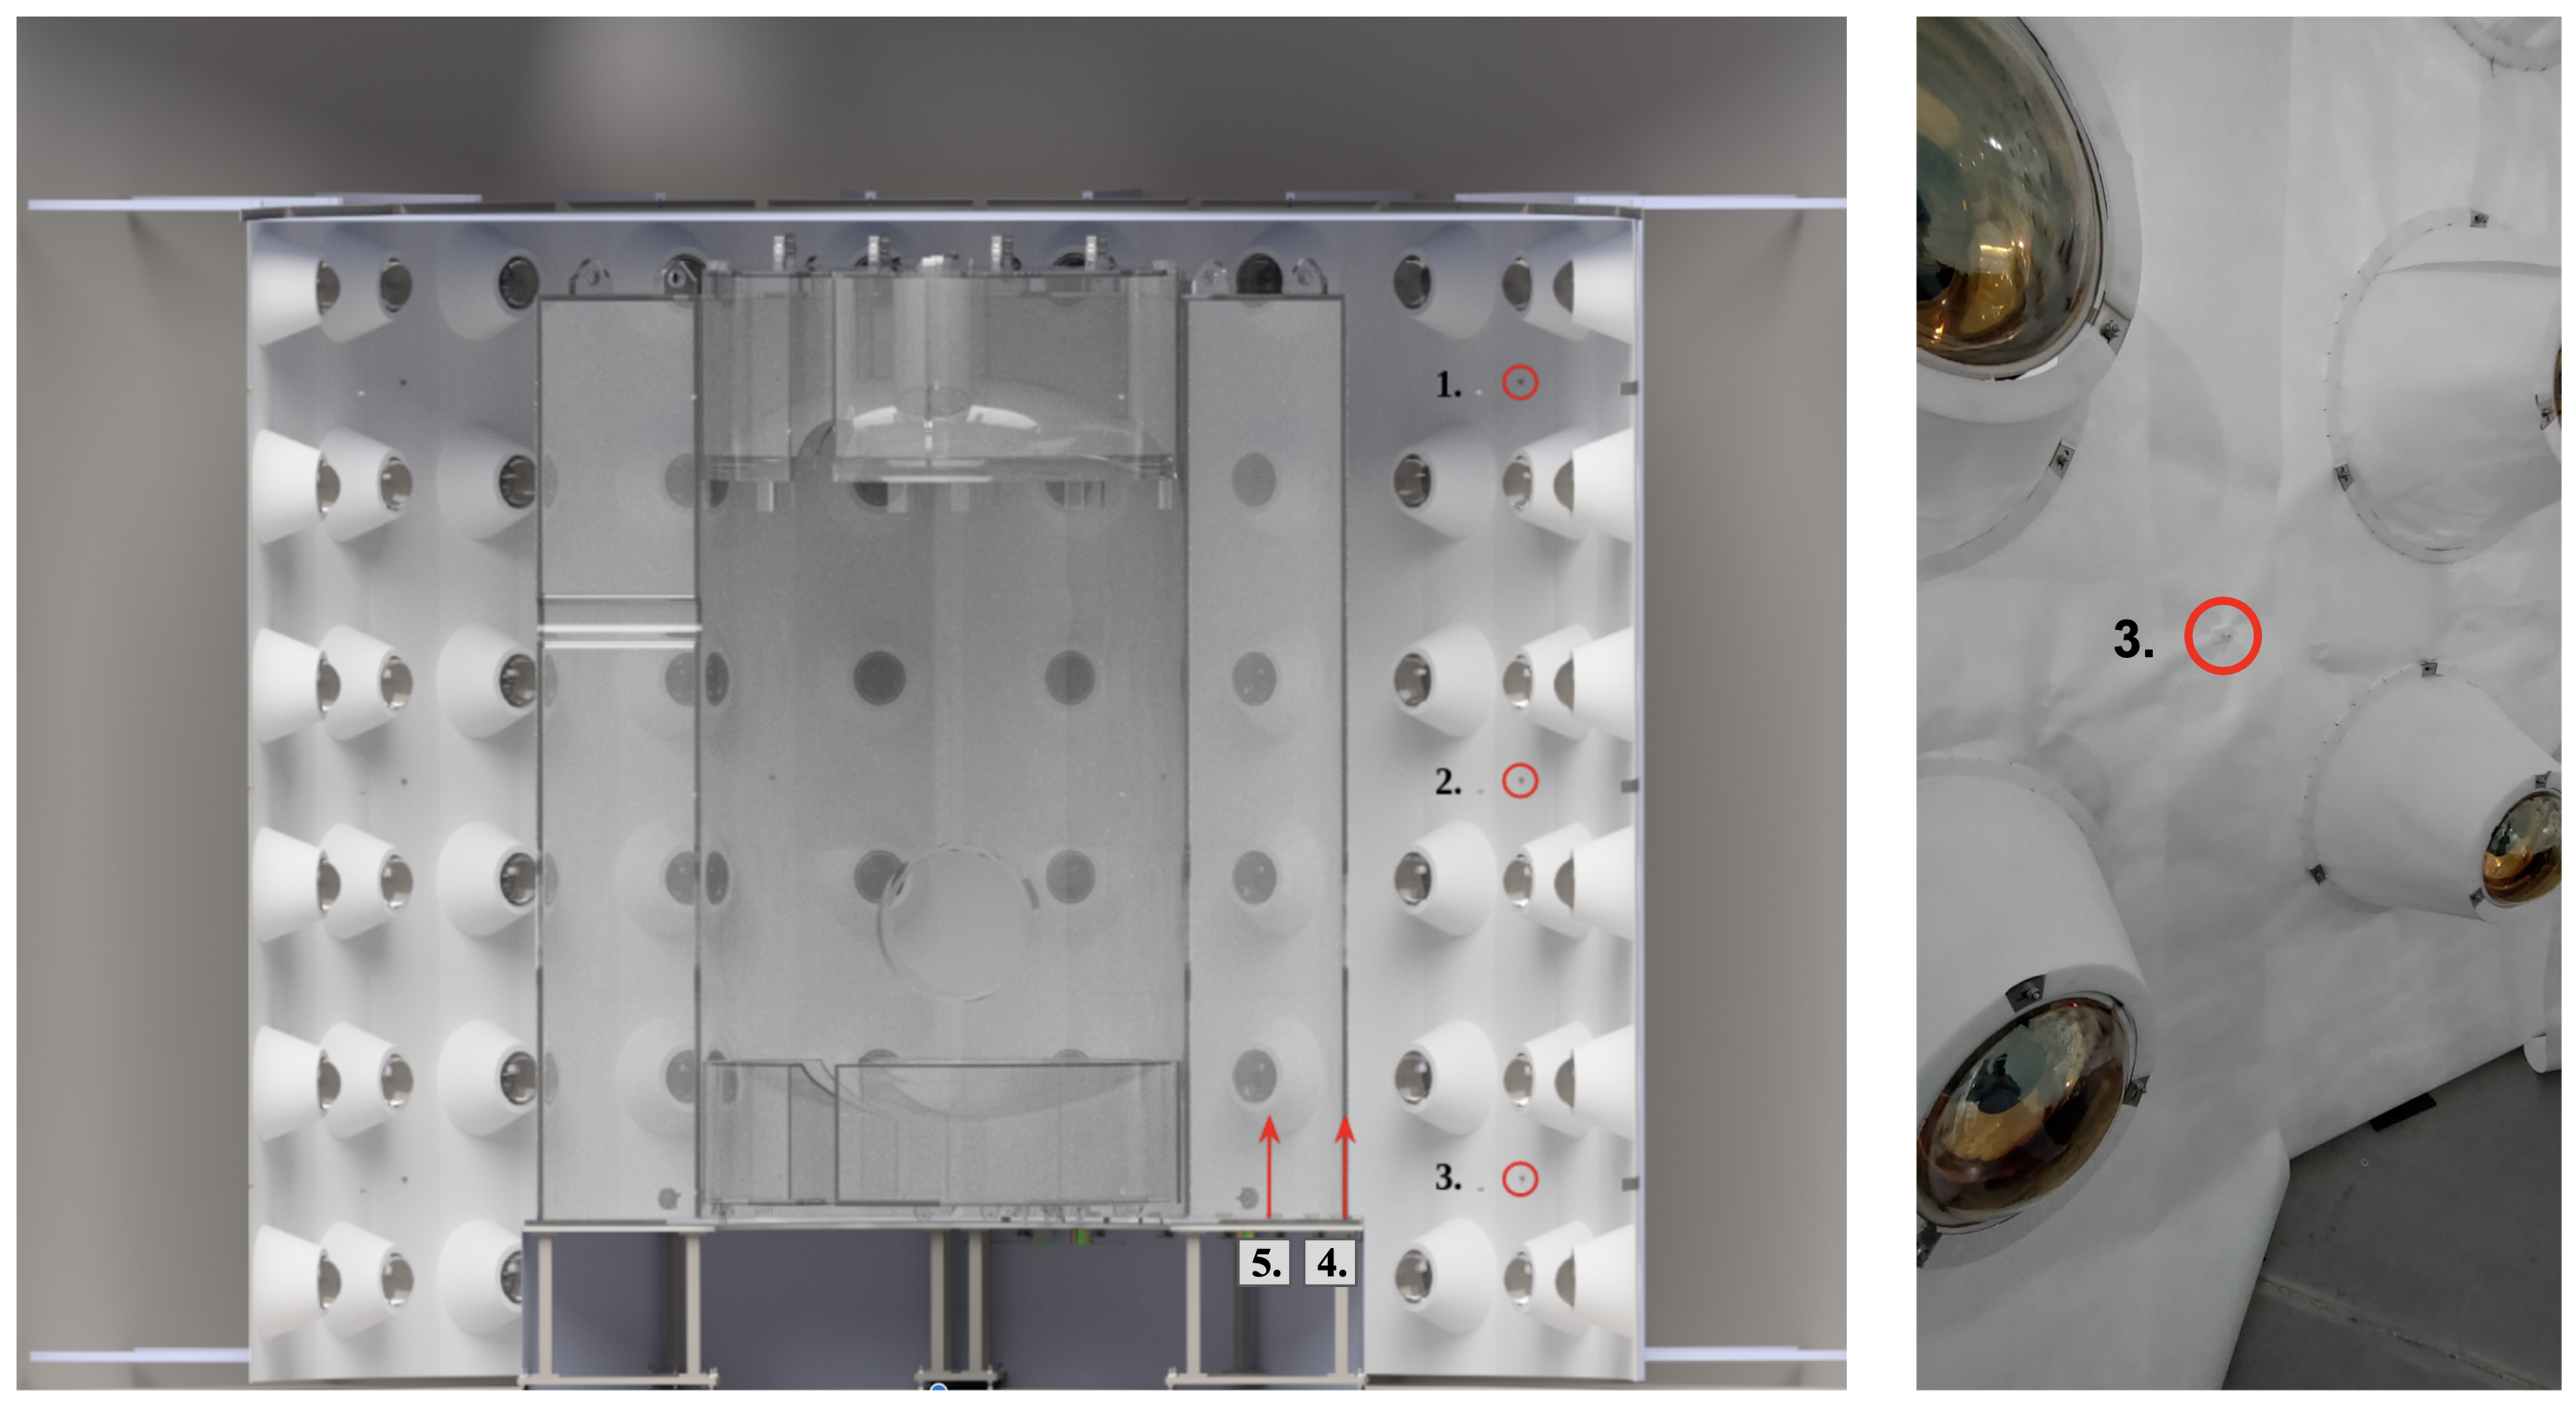
\includegraphics[width=\linewidth]{figures/LZ/OD_PMT_CAD_picture_v4.png}
    \caption{\textbf{Left:} A cross-section of a CAD drawing of the OD. The three  heights of the 10 azimuthal positions of the optical fibre injection points are labelled 1-3. Two injection positions under the side acrylic tanks which point upwards are labelled 4 and 5. \textbf{Right:} A photograph of the OD PMT array showing the point of an injection point relatively to the surrounding PMTs.}
    \label{fig:OCSPositions}
\end{figure}
Duplex fibres are used to inject light pulses produced by LEDs to the different locations. For the thirty injection points situated within the PMT, 435~nm LEDs are used to match the peak wavelength and quantum efficiency of OD PMTs. Only one core in the fibre is used, the additional core is a backup in the event of any damage to the first core. 435~nm and 450~nm were doing for the injection points facing into the LS to monitor optical degradation of the scintillator. Below 420~nm the absorption length of GdLS decreases significantly as shown in \autoref{fig:GdLSSpecRes}, if the scintillator degrades this region shifts to higher wavelengths. A similar approach is taken for monitoring the optical properties of the acrylic using 390~nm and 435~nm LEDs. The transmission of light through the acrylic varies with wavelength, as shown in \autoref{fig:AcrylicQA}. Monitoring the optical properties of the acrylic and scintillator during science runs is key to ensure consistent light collection during science runs.
\begin{figure}[h!]
    \centering
    \includegraphics[width=0.7\linewidth]{figures/LZ/T187-XDM-UVT_WAVELENGHT_08252017.png}
    \caption{Quality assurance measurement data taken during the commissioning of the acrylic tanks. The QA measurement data is the average transmission of light at a particular wavelength across 46 points. Vertical lines indicate the 390~nm and 435~nm LEDs with respect to the transmission of light.}
    \label{fig:AcrylicQA}
\end{figure}
The electronics system which controls the LEDs consists of five Optical Calibration Cards (OCC). Each OCC consists of an FPGA controlled motherboard which houses eight LED pulser boards and two four-channel photodiode boards. Light pulses from the LEDs are divided by a three-way optical coupler: to the injection points in the OD; to the photodiode readout for onboard monitoring; to a monitoring PMT. The layout of the system can be seen in \autoref{fig:OCSSchematic}.
\begin{figure}[h!]
    \centering
    \includegraphics[width=\linewidth]{figures/LZ/OCSSchematic_0.png}
    \caption{A schematic of the OD OCS. An example of one Optical Calibration Card (OCC) is shown with its eight LED pulser boards and two photodiode boards. A total of five OCCs make up the OCS and are powered by a VME crate. Lines with arrows show the paths light takes down various fibres to different positions in the system. Labels 1-3 represent the three heights within the PMT array, while Label 4-5 denote the injection points to monitor the GdLS/acrylic, as shown in \autoref{fig:OCSPositions}. Adapted from Ref.\cite{Turner:2021qvi,LZ:2024bsz}.
    \textcolor{red}{NEED TO CHANGE THE COLOURS IN THIS SCHEMATIC!}}
    \label{fig:OCSSchematic}
\end{figure}
The intensity of light is monitored using the onboard photodiode and rack mounted monitoring PMT, which is the same 8-inch Hamamatsu R5912 PMT as used in the OD PMT array \cite{Turner:2021qvi}. The stability of the light produced by the LEDs is monitored through the comparison of light produced by an in-situ YAP:Ce pulser which produces light pulses corresponding to 5000 photoelectrons \cite{Turner:2021qvi,KOBAYASHI1994355}. The intensity of light produced by both the LED and source is then compared for consistency across science runs. The commissioning of this subsystem is covered further in \autoref{chap:ODCommissioning}. The OCS is controlled through LZ's central Slow Control System, allowing a user to define a pulse size/intensity using a graphical user interface \cite{hbirch:thesis}.
During the authors Masters degree at the University of Liverpool a member of the group who developed the OCS and extensively tested the system. The OCS met all design requirements set by LZ \cite{Turner:2021qvi}. Further details of the OCS and the QA tests prior to installation can be found at Ref.\cite{hbirch:thesis,Turner:2021qvi}. 

\section{Calibration Systems and Sources}
To understand the LZ detector response and its performance, regular calibrations are performed using a variety of methods and sources. Such calibration procedures are used to characterise: the energy scale; energy threshold; micro physics of particle interactions; as well as the position and time dependence of the detector responses \cite{LZ:2024bsz}. A summary of the sources, their purpose and their deployment methods is shown in \autoref{tab:CalibrationSources}.
\begin{table}[h!]
    \centering
    \begin{tabular}{|c|c|c|c|c|}
         \hline
         Isotope & Interacting & Energy [keV] & Purpose & Deployment \\
         & Particle & & & \\
         \hline
         $^{83m}\text{Kr}$ & $\beta, \gamma$ & $32.1/9.4$ &TPC(x,y,z) & Injected\\
         $^{131m}\text{Xe}$& $\gamma$, x-ray & $163.9$ & TPC(x,y,z), Skin & Injected\\
         $^{220}\text{Rn}$& $\alpha,\beta,\gamma$ & Various \cite{Jorg:2023nvl} & Skin, ER Band & Injected\\
         $^{3}\text{H}$& $\beta$ & $0-18.6$ &ER Band & Injected\\
         $^{14}\text{C}$& $\beta$ & $0-156.4$ &ER Band & Injected\\
         $^{241}\text{AmLi}$& $(\alpha,n)$ & $(5638, 0-1500)$ & NR Band, Veto Efficiency & CSD\\
         $^{241}\text{AmBe}$& $(\alpha,n)$ & $(5638, 0-11\times10^{3})$ & NR Band, Veto Efficiency & CSD\\
         %$^{252}\text{Cf}$& Spontaneous Fission & &NR Efficency & External\\
         $^{57}\text{Co}$& $\gamma$ & $122$ &Skin Energy Scale & CSD\\
         $^{228}\text{Th}$& $\gamma$ & $2615$ &OD Energy Scale & CSD\\
         $^{22}\text{Na}$& $\gamma$ & $511, 1275$ &Inter-detector Timing & CSD\\
         $^{52}\text{Mn}$& $\gamma$ & $835$ &Skin Energy Scale & CSD\\
         $^{88}\text{YBe}$& $(\gamma,n)$ & $(1836,152)$ &NR Response & External\\
         $^{88}\text{YMg}$& $n$ & $1836$ & NR Response & External\\
         DD& $n$ & $2460$ & Light and Charge Yields & External\\
         $^{241}\text{Am}$& $\alpha$ & $5638$ &ODOCS Calibration & External\\
         \hline
    \end{tabular}
    \caption{A list of calibration source used by LZ for TPC, Skin and OD calibrations along with the purpose and method of deployment. The energy (keV) refers to particle energies relevant for the calibration of LZ and is not a complete list of decay energies. The energies quoted in the parentheses correspond to those of the particle species from the previous column. Adapted from Ref.\cite{LZ:2024bsz,lkorley:thesis}.}
    \label{tab:CalibrationSources}
\end{table}
Injected sources consist of gaseous radioisotopes which are injected into the xenon circulation system and in turn into the TPC volume itself. The injection of sources directly into the TPC volume is beneficial for a few reasons. Firstly, as source is injected and allow to mix with the LXe, this allows calibration with spatial uniformity. Secondly, the LXe target is self-shielding so an external low energy source would require a large amount of exposure time to achieve comparable statistics to the injected source. Lastly, monitoring how the injected isotopes mix within the TPC allows LZ to further understand the mixing and flow patterns of background radioisotopes \cite{LZ:2024bsz}. The injected radioisotopes either decay away due to their short-lived nature ($^{83m}\text{Kr}$,$^{131m}\text{Xe}$ and $^{220}\text{Rn}$) whereas the live-lived source, tritiated methane ($\text{CH}_4$, is removed by the hot zirconium getter \cite{LZNIMA}.

Beyond the injected sources, there are external sources which can be separated into two subcategories by their deployment, either using the Calibration Source Deployment system or stand alone deployment method. The CSD lowers neutron and gamma rod sources in three tubes located in the vacuum space between the ICV and OCV \cite{LZNIMA}. Each tube is connected to an independent deployment system which allows sources to be precisely positioned at different depths in the detector. Depending on the depth of deployment, the radioactive source can generate signals in various regions of the OD, TPC, and Skin. The use of various sources at various heights allows for calibration of the detectors' energy scale and the spatial dependence of the energy scale. Inter-detector timing measurements between the three detectors is also carried out using the CSD sources. Understanding time offsets between the detectors is crucial for functioning veto system which is dependent on time based section to remove background events.

Beside the CSD sources, a deuterium-deuterium (DD) neutron generator is used to produced neutrons for TPC calibrations and to cross check Veto tagging efficiency (discussed in \autoref{chap:VetoEfficiency}). The generator produces 2.45~MeV neutrons which are directed through calibration conduits that pass through the OD acrylic tanks to the OCV. A detailed description of neutron generation and the system is provided in Ref.\cite{LZ:2024bsz}. To understand low energy detection efficiency of the TPC $^{88}\text{YBe}$ and $^{88}\text{YMg}$ photo-neutron sources are used. Both sources are deployed externally through a removing a small acrylic vessel in the OD and replacing it with source assembly. This small vessel is shown in green above the blue top tanks in  \autoref{fig:ODTanks}.
The final source listed in \autoref{tab:CalibrationSources} is sealed $^{241}\text{Am}$ within a YAP:Ce crystal and is used within the ODOCS, as described in \autoref{sec:ODOCS}.

\section{Data Acquisition System}\label{sec:LZDAQ}
Signals produced in the PMTs across the experiment are processed by the data acquisition system. LZ employs a custom FPGA-based Architecture for Data Acquisition and Real time monitoring (FADR) to perform the digitisation and identify events of interest for offline analysis \cite{LZ:2024bvw,Druszkiewicz:2015pcl}. 
Signals first pass through shaping amplifiers which increases signal-noise ratio. At the amplifier stage, the signals from the TPC and OD are split into dual gain outputs to maximize the available dynamic range and extend the range of energies than can be probed by the experiment. The Skin detector has only a single gain output. Following amplification, the analogue signals are digitized with a sample rate of 100~MHz (10~ns samples) using custom built 32-channel digital signal processing boards \cite{Druszkiewicz:2015pcl}. Due to the sheer volume of data that comes from the PMTs Pulse Only Digitisation (POD) methods are employed to reduce the raw waveform volume by a factor of 50 \cite{LZTDR}. The threshold used in this filter is tuned on SPhE data and is set to provide a detection efficiency of $>99\%$ \cite{LZ:2024bvw}. Results from the POD waveform analysis are passed to the data sparsifiers and grouped by the Data Sparsifier Master (DSM) where a decision is made whether an event has been observed. The DSM informs the DAQ Master and time window is selected for the event and the data is extracted from the digitizers and stored by one of the Data Collectors. A simplified schematic of the LZ DAQ system is shown in \ref{fig:LZDAQ}, depicting one channel of digital electronics. Event builders take the data which has been temporarily stored on the Data Collectors, organized the data by channel, and assembles full event structures for offline analysis. \textcolor{red}{Should I include something on the triggers? FADR Paper P15 \cite{LZ:2024bvw}} An in-depth description of FADR can be found at Ref. \cite{LZ:2024bvw}.
\begin{figure}[h!]
    \centering
    \includegraphics[width=\linewidth]{figures/LZ/LZDAQ.png}
    \caption{A simplified schematic depicting how PMT signals are processed using the LZ DAQ system. Adapted from Ref.\cite{LZ:2024bvw}.}
    \label{fig:LZDAQ}
\end{figure}
\section{Simulation Techniques}
Simulations of the LZ experiment play a key role understanding the detector and its response. They present several purposes, for example: the calculation of background rates in LZ; the prediction of of sensitivity of the experiment to rare event searches through Profile Likelihood Ratio analysis (PLR); the testing of event reconstruction infrastructure; determining efficiencies of data selection methods. An overview of the LZ simulation framework is shown in \autoref{fig:LZSimFramework}.
\begin{figure}[h!]
    \centering
    \includegraphics[width=\linewidth]{figures/LZ/LZSimFramework.png}
    \caption{Simulation framework for the LZ experiment. ``Full'' and ``Fast'' simulation chains are shown. Both chains begin with BACCARAT and end with an output LZap RQ file.}
    \label{fig:LZSimFramework}
\end{figure}
For all simulations, LZ uses BACCARAT\footnote{\textbf{B}asically \textbf{A} \textbf{C}omponent-\textbf{C}entric \textbf{A}nalogue \textbf{R}esponse to \textbf{A}ny\textbf{T}hing}\cite{LZ_SIMS} package to simulate particle interactions in the detector and this package is built upon the GEANT4 simulation toolkit \cite{GEANT4:2002zbu}. Using GEANT4 along with CAD-Drawing, the LZ experiment is built as a detector geometry. In simulation, a series of inputs can be used to generate particles which are propagated through the detector geometry, with any additional particles being generated from interactions with detector materials. GEANT4 is used to track the particles and identifies the interaction points. From there, two separate chains exist for interpreting this information, \autoref{fig:LZSimFramework}.

The ``Fast'' chain, seen on the right of \autoref{fig:LZSimFramework}, records energy deposits in the detector and passes them to LZLAMA for processing. LZLAMA consists of two primary packages, the Noble Element Simulation Technique (NEST) to process interactions in the xenon space and DICEBOX to process interactions with the OD. NEST provides the expected conversion of energy to scintillation photons and ionization electrons based on empirical models developed using experiment measurements \cite{NEST1}. The DICEBOX toolkit is empolyed to handle interactions between neutrons and their capture on Gd as GEANT4 has difficulty conserving Q-value and multiplicity of the gamma emissions from the neutron capture. Energy deposits in other volumes are handled by GEANT4. LZLAMA outputs a ROOT file which has the same reduced-quantity (RQ) format as data processed using LZ's custom processing tool, LZap \cite{LZ_SIMS}, which performs pulse and event reconstruction.

The second, ``Full'' chain, enables full simulation of optical processes throughout the entire detector including VUV photons and ionisation electrons that are produced in the xenon and scintillation light generated in the OD. Another custom LZ software package, Detector Electronic Response (DER), is used to translate PMT hits in the BACCARAT output into waveforms. The DER simulates the analogue front-end electronics of LZ to produce waveforms, written in an identical format to the true LZ DAQ, \autoref{sec:LZDAQ}. A number of physical processes are incorporated into the DER to create realistic waveforms including: a PMT response model, gain, quantum efficiency, double photoelectron probability, dynode effects, dark rate, and afterpulsing. This chain is more computationally intensive but it allows for a more realistic, event-by-event analysis. The output from the DER is processed by LZap to produce RQ-structured files to be analysed much like real data.
A complete review of the LZ Simulation framework can be found at Ref.\cite{LZ_SIMS}.

\section{Assembly and Operation of the LZ Detector}
During the past six years whilst the author has collaborated on the LZ Experiment, a significant portion of that time has been spent on-site at SURF working on the assembly, commissioning and operation of the LZ Detector. These efforts began with the installation of the OCS electronics and an in-situ-calibration of the LED system, this work is detailed extensively in Ref.\cite{hbirch:thesis}.
\begin{figure}
     \centering
     \begin{subfigure}{0.41\textwidth}
         \centering
         \includegraphics[width=\textwidth]{figures/LZ/OCSMotherboardCC.png}
         \label{fig:Gonk0}
     \end{subfigure}
     %\hfill
     \begin{subfigure}{0.47\textwidth}
         \centering
         \includegraphics[width=\textwidth]{figures/LZ/OCSElectronicsInstallation.png}
         \label{fig:Gonk1}
         \caption{The author making serial connections between the front planes of the OCS OCCs within the electronics racks.}
     \end{subfigure}
     \caption{}
\end{figure}
\chapter{Outer Detector Commissioning and Monitoring}
\section{Single Photo-electron Calibration}

\section{Reconstructed Gain}
\subsection{Gain Curves}
\subsection{Monitoring PMT Health Over Time}

\section{Trigger Efficiency}

\section{Optical Calibration System Development}
\subsection{UV LED commissioning}

\subsection{Monitoring PMT}
\chapter{Veto efficiency studies for the 2024 WIMP search result}\label{chap:VetoEfficiency}
A WIMP scatter is expected to only deposit a small amount of energy (few~keV) within the LXe volume of the experiment in a single scatter. Neutrons produced through radioactive decays within detector materials mimics a WIMP interaction when they scatter off Xe atoms. Veto detectors surrounding the central LXe volume also permits assessment of the local radioactivity environment, and thus to infer additional information on the backgrounds in the WIMP search region. A WIMP discovery will require excellent understanding of all background sources, which is best done through the characterization of those backgrounds in situ. Efficiency of the veto systems in the detection of the radiation produced by the backgrounds should be maximised whilst minimizing the impact of the veto selection on detector livetime in turn maximising the detector livetime available for the detection of WIMPs. \autoref{sec:VetoEff/simulation_improvements} describes the series of improvements to the detector simulation which were made prior to the WS2024 science run which aided the understanding of the response from the veto detector systems. The refinement of the veto selection algorithm is discussed alongside the impact that the veto selection had on the WS2024 result from \autoref{sec:VetoEff/VetoSelectionOptimisation} onwards.

\section{Improved Outer Detector Simulations}\label{sec:VetoEff/simulation_improvements}
Prior to WS2024 result, there were a number of major differences between simulations and data in the Outer Detector (OD). As such, an effort was made to correct this through modifications to the geometry of the Outer Detector in simulations to better reflect what is observed in data.
\subsection{Modifications of the Outer Detector simulation geometry}\label{sec:VetoEff/GeometryEdits}
There was a distinct discrepancy in neutron capture timing following single scatters within the TPC, this was one of the metrics which was investigated to quantify difference between data and simulation.
The simulation was improved through the following changes:
\begin{enumerate}
	%\item Spacing was added between the acrylic tanks to account for the gaps between the tanks which were present due to minor geometric differences produces in the moulding of the vessels during manufacturing process.
	\item Water was added to the foam volume which is between the OCV and acrylic tanks. The foam was intended to displace water to reduce neutron capture time however the foam became saturated with water \footnote{Later long-term bench top studies found that samples of foam became saturated with water.}.
	\item The acrylic tanks were moved further away from the OCV in the simulation to reflect the actual position of the tanks in the Outer Detector, as installed.
\end{enumerate}
A series of simulations were produced varying both the amount of water saturation of foam displacer in 1\% steps and the position of the acrylic tanks from the OCV in 10~mm steps. The \textit{best} configuration of the simulation geometry changes was found to be 30~mm and 6\% through matching the capture time of neutrons following single scatters in the active LXe volume. Additional details on the discrepancies between simulations and data with respect to neutron capture timing is given in the subsequent subsection.
\begin{figure}[ht!]
	\centering
	\includegraphics[width=0.9\textwidth]{figures/VetoEfficiency/FoamImgAndSimGeoTogether.png}
	\caption[An image of the foam displacer surrounding the OCS and final geometry in the simulation used for the WS2024 science run.]{Geometry in the simulation used for the WS2024 science run. \textbf{Left:} A photograph of the light green foam water displacer which resides between the acrylic tanks and the OCV. The water displacer was wrapped in a light reflector made from Tyvek. \textbf{Right:} A cross-section of the BACCARAT output. Geantinos were been passed through the simulation geometry, the $xyz$ position information and GEANT4 volumes were recorded to show the various volumes in the simulation.}
	\label{fig:VetoEff/od_geometry_for_sr3}
\end{figure}

\subsubsection{Neutron capture time}\label{sec:VetoEff/NCT}
Following the geometry changes discussed above, the neutron capture timing using AmLi was studied. Events which were classified as single scatters by LZap and passed the selection outlined in \autoref{tab:App_VetoEff/CoreCuts} in \autoref{app:VetoEff} were used for the study. OD pulses which exceeded a 200~keV (49~phd) threshold were used to optimise the geometry as this threshold is associated with proton recoil of neutrons of hydrogen in the OD medium.
All possible configurations of the geometry modifications were visually examined to determine which variation of simulation matched the data. An example of the comparison plot can be seen in \autoref{fig:VetoEff/NC_AmLi_50mm7}, the "baseline simulation" was the initially configuration of the geometry prior to this study. All plots were examined side by side in a large scale canvas configuration seen in Fig.\ref{fig:VetoEff/NC_Canvas0}, \ref{fig:VetoEff/NC_Canvas1}, \ref{fig:VetoEff/NC_Canvas2}, and \ref{fig:VetoEff/NC_Canvas3}. It was found that from this study that 30~mm~to~50~mm movement of the SATs alongside 5\%~to~7\% increase in the percentage of water in the foam provides the best agreement between data and simulation at a 200~keV threshold.
\begin{figure}[!ht]
	\centering
	\includegraphics[width=0.7\linewidth]{figures/VetoEfficiency/movedSAT50mm_7percentWater_AmLi_CSD3_Z700mm_200keV_Ratio.png}
	\caption{An example of the plot used to compare neutron capture timing in data with the baseline simulation and the modified simulation. The relative change between data and simulation in each $20~\mu s$ bin was used to aid the visually examination across the $1200~\mu s$ window.}
	\label{fig:VetoEff/NC_AmLi_50mm7}
\end{figure}

\iffalse
\begin{sidewaysfigure}[ht!]
	\centering
	\includegraphics[width=\linewidth]{figures/VetoEfficiency/NCTiming_Canvas_700mm_AmLi.pdf}
	\caption{Large scale canvas of all possible simulation configurations. Each plot is similar in style to \autoref{fig:VetoEff/NC_AmLi_50mm7}. Here AmLi at 700mm above the cathode in CSD3 has been shown as an example.}
	\label{fig:VetoEff/NC_Canvas}
\end{sidewaysfigure}
\fi

\section{Veto selection optimisation}\label{sec:VetoEff/VetoSelectionOptimisation}
A description of how the veto selection for the WS2024 was optimised is presented in this section. The Skin and OD veto cuts used in the WS2024 science run were based on those developed for the WS2022 science run, described in \cite{LZCollaboration:2024lux} and are presented in \autoref{tab:VetoEff/sr3_veto_cuts}.
The veto selection relies on four separate selection criteria which each have their own intended purposes:
\begin{itemize}
	\item \textit{Skin-prompt} used for tagging $\gamma$-rays in the Skin detector
	\item \textit{OD-prompt} used for tagging $\gamma$-rays and neutron proton recoils in the OD
	\item \textit{Skin-delayed} used for tagging $\gamma$-rays from post-neutron capture de-excitation
	\item \textit{OD-delayed} used For tagging $\gamma$-rays from post-neutron capture de-excitation
\end{itemize}
The cuts used for the different veto criteria were selected at the same time as AmLi neutron tagging efficiency calculation, and were optimised to maximise the tagging efficiency whilst reducing deadtime. \textit{Pulse area} threshold, \textit{PMT coincidence} threshold and \textit{veto window length} are the three different variables which can be tuned for this optimisation. Events which were classified as single scatters by LZap and passed the selection outlined in \autoref{tab:VetoEff/amli_efficiency_cuts} were used for the study. The following subsections describe how each of the veto selection variables were tuned.

\begin{table}[!ht]
	\centering
	\caption{Outline of cuts applied to AmLi calibration data for determining the veto efficiency. All cuts are defined in \autoref{tab:App_VetoEff/CoreCuts}.}
	\label{tab:VetoEff/amli_efficiency_cuts}
    \scalebox{0.9}{
	\begin{tabular}{llll}
    \hline\hline
    \textbf{Livetime cuts}&\textbf{ Physics cuts}& \textbf{S2 cuts}& \textbf{S1 cuts}\\
    \hline
    Burst noise cut& Single scatter& S2 width vs drift time& S1 prominence cut\\
    Muon holdoff& S1 and S2 threshold & Narrow S2& Stinger event cut\\
    Sustained rate cut& Fiducial Volume& S2 rise time& S1 TBA vs drift time \\
    High S1 rate exclusion & & S2 early peak& S1 HSC cut\\
    Bad buffer cuts& & S2 XY quality& S1 shape\\
    Excess Area cut& & S2 TBA & S1 photon timing\\
    \hline\hline
	\end{tabular}}
\end{table}

\subsection{Veto window length}
The veto window length for the prompt windows were determined using AmLi and DD calibration data by measuring the time difference between the TPC single-scatter and OD and Skin pulses. The length of the prompt window is determined by width of the peak observed in the pulse timing distributions shown in both figures in \autoref{fig:VetoEff/veto_prompt_windows}. For the WS2024 selection, no change was made to the OD prompt veto window size, however the Skin prompt veto window was reduced by 500~ns as the number of the pulses observed outside of window $\pm250$~ns was considered negligible.
\begin{figure}[!ht]
	\centering
	\begin{subfigure}[b]{0.49\textwidth}
		\centering
		\includegraphics[width=\textwidth]{figures/VetoEfficiency/ODpromptWindowTiming.pdf}
		%\caption{Time difference (in ns) between TPC single-scatter and OD pulses using AmLi data.}
        \caption{}
		\label{fig:VetoEff/od_prompt_window}
	\end{subfigure}
	\hfill
	\begin{subfigure}[b]{0.49\textwidth}
		\centering
		\includegraphics[width=\textwidth]{figures/VetoEfficiency/SkinpromptWindowTiming.pdf}
		%\caption{Time difference (in ns) between TPC single-scatter and OD pulses using DD data.}
		\caption{}
        \label{fig:VetoEff/skin_prompt_window}
	\end{subfigure}
	\caption{Prompt timing window for the OD (left) and Skin (right). %The time difference between TPC single scatter pulse and veto pulse was used to determine the optimal veto window size. 
    AmLi (blue) and DD (orange) calibration data was used to measure the time difference between the TPC single scatter pulse and veto pulse. 
    The vertical red lines indicate the boundary of the timing selection used for WS2024. There was no change in the size of the OD prompt veto window whereas the Skin prompt veto window was reduce by a total of 500~ns. The WS2022 veto window limits are shown in green.}
	\label{fig:VetoEff/veto_prompt_windows}
\end{figure}

The veto efficiency (defined in \ref{eqn:VetoEff/neutron_tagging_efficiency}) calculated using AmLi calibration data was used to determine the size of the delayed veto window for both the Skin and OD. The veto window length was reduced by a factor of two for both Skin and OD delayed windows as the slope of the efficiency curve began to plateau above 600~$\mu s$. An example of the veto efficiency plot used is shown in \autoref{fig:VetoEff/DelayedVetoWindow}.
\begin{figure}[!ht]
    \centering
    \includegraphics[width=0.5\linewidth]{figures/VetoEfficiency/DelayedVetoWindow.pdf}
    \caption{An example of a veto efficiency curve measured using AmLi calibration data. The vertical red line indicates the WS2024 upper bound of the delayed veto windows used for both the Skin and OD.}
    \label{fig:VetoEff/DelayedVetoWindow}
\end{figure}

The reduction in the veto window lengths has a positive impact on the dead time induced by the veto selection. Veto dead time is discussed in greater detail \autoref{sec:VetoEff/DeadtimeStability}.

\subsection{PMT Coincidence and pulse area threshold}
To optimize the pulse area and PMT coincidence thresholds the veto efficiency and deadtime was calculated for different integer step changes of both the pulse area and PMT coincidence for the respective veto windows. Heatmaps of efficiency and deadtime based on PMT coincidence and pulse area threshold were produced, an example of a heatmap is shown in \autoref{fig:VetoEff/od_prompt_veto_heatmap}. All heatmaps produced for the optimization study are shown in \autoref{app:VetoHeatMapsSec}.

\begin{sidewaysfigure}
	\centering
	\includegraphics[width=\textwidth]{figures/VetoEfficiency/Heatmap600us_ODDelayedSkinDelayedThresholds.png}
	\caption{Heatmap used to determine optimal OD and Skin Delayed thresholds based on efficiency.
		The z-axis shows the efficiency associated with a given pulse area requirement for the delayed veto windows defined in \autoref{tab:VetoEff/sr3_veto_cuts}.
	}
	\label{fig:VetoEff/od_prompt_veto_heatmap}
\end{sidewaysfigure}

Compiling the heatmaps of efficiency and deadtime for established veto windows of the different criteria, thresholds were chosen to maximise efficiency whilst minimising dead time. An example plot used to determine this is shown in \autoref{fig:VetoEff/veto_cut_optimisation}.
For the WS2024 science run, the approach of trying to maintain the efficiency of WS2022 veto of $\sim$~89\%, whilst reducing the livetime impact was taken. It was determined that the efficiency could be matched to the veto efficiency achieved in the WS2022 science run whilst achieving a factor of two reduction in deadtime.

\noindent
The final cuts for the WS2024 science run are shown in \autoref{tab:VetoEff/sr3_veto_cuts}, with the WS2022 selection included for comparison.

\iffalse
\begin{sidewaysfigure}
	\centering
	\includegraphics[width=\textwidth]{figures/VetoEfficiency/HeatmapSkinPACoinScanWindow500.pdf}
	\caption{Skin Prompt heatmap.
		In each bin, either the pulse coincidence or the pulse threshold has been varied.
		The z-axis shows the efficiency associated with a given pulse requirement.
		The veto time window considered is [-250, 250]ns.}
	\label{fig:VetoEff/skin_prompt_veto_heatmap}
\end{sidewaysfigure}
\begin{sidewaysfigure}
	\centering
	\includegraphics[width=\textwidth]{figures/VetoEfficiency/OD_Deadtime_thesis.png}
	\caption{OD Delayed heatmap.
		In each bin, either the veto window or the pulse threshold has been varied.
		The z-axis shows the deadtime associated with a given veto window and pulse threshold.
		In addition to the pulse area threshold, the pulse must have a coincidence greater than 5.}
	\label{fig:VetoEff/od_delayed_veto_heatmap}
\end{sidewaysfigure}
\begin{sidewaysfigure}
	\centering
	\includegraphics[width=\textwidth]{figures/VetoEfficiency/Skin_Deadtime_thesis.png}
	\caption{Delayed vetoes heatmap.
		In each bin, the OD pulse threshold or the Skin pulse threshold has been varied.
		The z-axis shows the veto efficiency associated with a given pulse thresholds.
		In addition to the pulse area threshold, the OD pulse must have a coincidence greater than 5, and the Skin pulse greater than 2.
		The veto window in this case is 500$\mu$s.}
	\label{fig:VetoEff/skin_delayed_veto_heatmap}
\end{sidewaysfigure}
\fi

\begin{figure}[!ht]
	\centering
	\includegraphics[width=0.6\textwidth]{figures/VetoEfficiency/DeadEffThresholdTest.pdf}
	\caption[Example plot used to highlight a number of considered cuts for the delayed Skin and OD pulse area thresholds for a 600~$\mu$s window.]{Example plot used to highlight a number of considered cuts for the delayed Skin and OD pulse area thresholds for a 600~$\mu$s window. The efficiency values have not been corrected for accidental coincidences. At each point, the numbers in brackets are the OD threshold pulse area, and the Skin threshold pulse area.}
	\label{fig:VetoEff/veto_cut_optimisation}
\end{figure}

\iffalse
\begin{figure}[!ht]
	\centering
	\includegraphics[width=0.9\textwidth]{figures/VetoEfficiency/sr3_cuts.png}
	\caption{Cuts determined to be optimal for the WS2024 science run.
		The WS2022 cuts are also included, where any modifications made to the selections is highlight accordingly.}
	\label{fig:VetoEff/sr3_veto_cuts}
\end{figure}
\fi

\begin{table}[!ht]
    \centering
    \caption{Cuts determined to be optimal for the WS2024 science run. The WS2022 cuts are also included, where any modifications made to the selections is shaded accordingly.}
    \label{tab:VetoEff/sr3_veto_cuts}
    \scalebox{0.9}{
    \begin{tabular}{|c|c|c||c|c|c|}
    \hline
    \multicolumn{3}{|c||}{\textbf{Skin Prompt}} & \multicolumn{3}{c|}{\textbf{OD Prompt}} \\
    \hline
    & WS2024 & WS2022 & & WS2024 & WS2022 \\
    \hline
    Window & \cellcolor[HTML]{cecece} [-250,250]~ns & \cellcolor[HTML]{cecece}[500,500]~ns & Window & [-300,300]~ns & [-300,300]~ns\\
    Coincidence&$>2$&$>2$&Coincidence&$>5$&$>5$\\
    Pulse Area & $>2.5$ & $>2.5$ & Pulse Area & \cellcolor[HTML]{cecece}$>4.5$ &\cellcolor[HTML]{cecece} $>0$ \\    
    \hhline{|===||===|}
    \multicolumn{3}{|c||}{\textbf{Skin Delayed}} & \multicolumn{3}{c|}{\textbf{OD Delayed}} \\
    \hline
    &WS2024&WS2022&&WS2024&WS2022\\
    \hline
    Window&\cellcolor[HTML]{cecece}[250~ns, 600~$\mu$s]&\cellcolor[HTML]{cecece}[500~ns, 1200~$\mu$s]&Window&\cellcolor[HTML]{cecece}[300~ns, 600~$\mu$s]&\cellcolor[HTML]{cecece}[300~ns, 1200~$\mu$s]\\
    Coincidence&\cellcolor[HTML]{cecece}$>2$&\cellcolor[HTML]{cecece}$>55$&Coincidence&$>5$&$>5$\\
    Pulse Area&\cellcolor[HTML]{cecece}$>46$&\cellcolor[HTML]{cecece}$>50$&Pulse Area&\cellcolor[HTML]{cecece}$>32.0$&\cellcolor[HTML]{cecece}$>37.5$\\
    \hline
    \end{tabular}}
\end{table}

\subsection{Deadtime stability}\label{sec:VetoEff/DeadtimeStability}
The stability of the induced deadtime for each of the veto selection windows over the WS2024 science run was assessed for stability by comparing the deadtime at monthly intervals. For each month, the rate of pulses in the Skin and OD, using the second half of the Random Trigger data was used; and the rate above the threshold, defined by the specific veto cut, was recorded. The stability of measured deadtime over the WS2024 science run is shown in \autoref{fig:VetoEff/deadtime_stability}.
The deadtime is then calculated as:
\begin{equation}
	\textrm{Dead Time [\%]} = 100 - (\lambda(x)\cdot t_{\text{vw}})
\end{equation}
where $\lambda(x)$ is the background rate above the veto threshold $x$, and $t_{\text{vw}}$ represents the veto window length measured in ns.
The conclusion that the deadtime is stable over the WS2024 science run was confirmed by looking at the rate of OD pulses above $200~\text{keV}$ (as defined by the WS2022 energy calibration) using the \lstinline{ODHealth} PREM module. No significant fluctuation was observed during WS2024 science run, shown in \autoref{fig:VetoEff/deadtime_stability_prem}.
\begin{figure}[!ht]
	\centering
	\includegraphics[width=0.7\textwidth]{figures/VetoEfficiency/SR3DeadTimeAll_withMean.pdf}
	\caption[Deadtime from the Skin and OD veto selection criteria during each month of WS2024 science run.]{Deadtime from the Skin and OD veto selection criteria during each month of WS2024 science run. The error shown in purely statistical and the mean across the science run is shown by a dashed line.}
	\label{fig:VetoEff/deadtime_stability}
\end{figure}
\begin{figure}[!ht]
	\centering
	\includegraphics[width=\textwidth]{figures/VetoEfficiency/prem_od_stability.png}
	\caption[Rate of OD pulses above 200~keV over the WS2024 science run.]{Rate of OD pulses above 200~keV (as defined by WS2022 energy calibration) over the WS2024 science run. Various periods of calibration are indicated by the coloured regions. {\color{red}Ewan to help make new plot with sidebar.}}
	\label{fig:VetoEff/deadtime_stability_prem}
\end{figure}

\section{Neutron veto efficiency}\label{sec:VetoEff/efficiency}
In this section, the efficiency of tagging background neutrons using the Skin and OD detectors is calculated.
This is performed by calculating the efficiency on AmLi and DD calibration data and comparing to simulations.
The difference between efficiencies from simulations and data is then used to calculate an offset.
The efficiency is then calculated for detector NR simulations and the observed offset is used as a correction factor to estimate the tagging efficiency for events classified as detector NR \cite{LZ:2022ysc,LZ:2024zvo}.
The efficiency is defined as:
\begin{equation}\label{eqn:VetoEff/neutron_tagging_efficiency}
	\eta\;[\%] = \frac{\textrm{N. Events passing Analysis Cuts + Veto Cuts}}{\textrm{N. Events passing Analysis Cuts}} \times 100
\end{equation}
and the inefficiency is defined as $\cancel{\eta}=100-\eta$. For all veto efficiency calculations in this chapter, if a pulse in the Skin or OD passes any of the selections outlined in \autoref{tab:VetoEff/sr3_veto_cuts}, then the event is included in the number of events in the numerator of \autoref{eqn:VetoEff/neutron_tagging_efficiency}. The efficiency based on this decision logic is the \textit{total veto efficiency}.

Two additional efficiencies were investigated: \textit{delayed veto efficiency} defined as events where a pulse is observed that fulfils either of the Skin delayed or OD delayed selection criteria, denoted by $\eta_\text{delayed}$; and \textit{OD-delayed veto efficiency} defined as events where a pulse is observed that fulfils the OD delayed selection criteria, denoted by $\eta_\text{OD-delayed}$.

Unless otherwise stated, all veto efficiencies presented follow the \textit{total veto efficiency} logic.

\subsection{Neutrons from calibration sources}
LZ utilises two neutron sources to measure the neutron tagging efficiencies of the veto detectors. AmLi sources are a compound of \textsuperscript{241}Am $\alpha$-radioactivity and \textsuperscript{7}Li produce low-energy neutron emission via nuclear $(\alpha,\text{n})$ reactions. Alphas from $^{241}$Am decay bombard the $^{7}$Li nuclei. This leads to a nuclear reaction of type \textsuperscript{7}Li$+\alpha \rightarrow$\textsuperscript{11}B\textsuperscript{*}. The excited \textsuperscript{11}B nucleus then decays to \textsuperscript{11}B via neutron emission. The neutrons produced by the AmLi sources have a maximum energy of $\sim1.5~\text{MeV}$ which results in a nuclear recoils depositing up to $\sim45~\text{keV}_{nr}$ of energy \cite{LZ:2024bsz}. Gamma radiation is also emitted in the \textsuperscript{241}Am decay to various states of \textsuperscript{237}Np and is an associated background to the reaction neutrons. The neutron to gamma ray emission ratio is 0.032 \cite{Sazzad:2023uqs}. The gamma ray background of the AmLi source is accounted for by the accidental correction factors described in \autoref{sec:VetoEff/AmLiAccCorrection}. The characterisation of the LZ AmLi sources is shown in Ref.~\cite{Sazzad:2023uqs}.

A deuterium-deuterium (DD) neutron generator is used to produce mono-energetic 2.46~MeV neutrons which result in nuclear recoils depositing up to $74~\text{keV}_{nr}$ of energy. Neutrons are produced by the DD generator as follows: Deuterium is ionized and turned into a plasma by a microwave. Deuterium ions in the plasma are accelerated towards a charged titanium-coated cooper target. D\textsuperscript{+} ions embed into the target form titanium deuteride. Subsequent D\textsuperscript{+} ions fuse to the embed ions and release neutrons via the D+D$\rightarrow$\textsuperscript{3}He+n. The generator is position outside of the water tank and neutrons are collimated and transmitted to the OCV through nitrogen purged conduits \cite{LZ:2024bsz}. The neutron production is pulsed to suppress the ER background rate and enables selection of events coincident with neutron production. Neutron pulsing decreases the impact of accidental coincidences which artificially increases the veto tagging efficiency. Accidental correction factors are still required as pulsing neutron production does not completely suppress accidental coincidences.

\subsubsection{AmLi}\label{sec:VetoEff/AmLi_Efficiency}
AmLi calibration data used is this study was taken during the May 2023 calibration campaign prior to the WS2024 science run. Events which were classified as single scatters by LZap and passed the selection outlined in \autoref{tab:VetoEff/amli_efficiency_cuts} were used for the study. Two additional cuts were applied to the calibration data:
\begin{enumerate}
	\item \textit{CSD tube position selection:} A circular cut on the reconstructed position of the SS S1 pulse in the TPC such that events from just one CSD tube are selected at a time. During the calibration campaign, sources were simultaneously deployed in each of the CSD tubes at equal heights (three separate height positions were used, $z=100~\text{mm},700~\text{mm},1300~\text{mm}$ relative to cathode at $z=0~\text{mm}$). Whereas separate simulations were produced with a single source in each CSD tube at three different heights (equal to the $z$-position used in the calibration campaign). 
    The circular cut selects events that have an SS S1 reconstructed position within a 50~mm radius of the CSD tube using the following equation:
    \begin{equation}\label{eqn:VetoEff/CSDSelection}
        \sqrt{(\text{S1}_x-\text{CSD}_x^i)^2+(\text{S1}_y-\text{CSD}_y^i)^2}<50
    \end{equation}
    where S1$_{x,y}$ is the reconstructed $(x,y)$-position of the S1 pulse in the SS and $\text{CSD}_{x,y}^i$ is the $(x,y)$-position of CSD where $i=1,2,3$ for each of the three CSD tubes.
    The boundaries of the cuts for each of the CSD tubes is shown in \autoref{fig:VetoEff/CSDSelection}. 
    \begin{figure}[!ht]
    \centering
        \includegraphics[width=0.7\textwidth]{figures/VetoEfficiency/CircularCSDCut.pdf}
        \caption{X-Y distribution of SS S1 pulses in the TPC for AmLi sources positioned at 700mm. Each of the circular cuts are overlaid on the plot.}
        \label{fig:VetoEff/CSDSelection}
    \end{figure}
    The position dependence of the veto efficiency can be examined by applying the CSD tube selection to data collected at different $z$-positions. The veto efficiency for different CSD tubes and $z$-positions is shown in \autoref{fig:VetoEff/VetoEffPositionDependence}.
    \begin{figure}[!ht]
    	\centering
    	\begin{subfigure}[b]{0.49\textwidth}
    		\centering
    		\includegraphics[width=\textwidth]{figures/VetoEfficiency/Eff_AmLi_Total_AllCSD.pdf}
    		\caption{}
            \label{fig:VetoEff/VetoEffPositionDependenceZPos}
    	\end{subfigure}
    	\hfill
    	\begin{subfigure}[b]{0.49\textwidth}
    		\centering
    		\includegraphics[width=\textwidth]{figures/VetoEfficiency/Eff_AmLi_Total_AllHeights.pdf}
            \caption{}
    		\label{fig:VetoEff/VetoEffPositionDependenceCSD}
    	\end{subfigure}
    	\caption{Position dependent veto efficiencies for different CSD tubes (left) and $z$-positions (right).}
    	\label{fig:VetoEff/VetoEffPositionDependence}
    \end{figure}
	A concern of this cut is that events towards the centre of the TPC are excluded. When the efficiency is averaged across different heights and CSD tube, the average can then be replicated in both data and simulation. 
    The position-averaged efficiency when the CSD cut is applied is $(88.21\pm1.03)\%$, whereas without the cut, the efficiency is $(88.25\pm1.22)\%$.
	The cut has $<5\%$ impact across the veto window and $<0.1\%$ impact at the 600~$\mu$s veto window threshold. This comparison is shown in \autoref{fig:VetoEff/CSDSelectionEffComp}.
    \begin{figure}[!ht]
    	\centering
    	\includegraphics[width=0.7\linewidth]{figures/VetoEfficiency/CSDSelectionCheck.pdf}
    	\caption[CSD tube selection impact on veto efficiency.]{CSD tube selection impact on veto efficiency. The average veto efficiency for events which have a reconstructed position with 50~mm of a CSD tube (blue) is compared to veto efficiency of all events with no CSD selection applied. The cut has $<5\%$ impact across the veto window and $<0.1\%$ impact at the 600~$\mu$s veto window threshold.}
    	\label{fig:VetoEff/CSDSelectionEffComp}
    \end{figure}

	\item \textit{NR-band selection:} SS events which have a S1 and S2 pulse area which lie within 1-$\sigma$ of NR band mean are selected to be used in the veto efficiency calculation.
    The NR bands are generated using the Noble Element Simulation Technique (NEST) \cite{NEST2011} are shown in \autoref{fig:VetoEff/SR3NRBands}. 
    The selection is defined as:
    \begin{equation}\label{eqn:VetoEff/NRBandSelection}
        -1<\frac{log_{10}(\text{S2}_\text{obs.})-\overline{log_{10}(\text{S2})}(\text{S1}_\text{obs.})}{\sigma_{log_{10}(\overline{\text{S2}})}(\text{S1}_\text{obs.})}<1
    \end{equation}
    where $\text{S1}_\text{obs.}$ and $log_{10}(\text{S2}_\text{obs.})$ are the observed pulse areas from the SS, $\overline{log_{10}(\text{S2})}(\text{S1}_\text{obs.})$ is the mean S2 corresponding to a observed S1 with $\sigma_{log_{10}(\overline{\text{S2}})}(\text{S1}_\text{obs.})$ based on the NEST model. The purpose of this cut is to improve the purity of the selection. 
    \begin{figure}[!ht]
    \centering
    \begin{subfigure}[b]{0.49\textwidth}
        \centering
        \includegraphics[width=\textwidth]{figures/VetoEfficiency/NRBands.pdf}
        \caption{}
        \label{fig:VetoEff/SR3NRBands}
    \end{subfigure}
    \hfill
    \begin{subfigure}[b]{0.49\textwidth}
        \centering
        \includegraphics[width=\textwidth]{figures/VetoEfficiency/AmLi700_NRBands.pdf}
        \caption{}
        \label{fig:VetoEff/AmLi700_NRBands}
    \end{subfigure}
    \caption{\textbf{Left:} The NR band means (solid line) with 1-$\sigma$ boundaries (dashed lines) for AmLi and DD calibration sources and a flat beta ER band mean with 1-$\sigma$ boundary. Both NR and ER bands and 1-$\sigma$ boundaries were generated using NEST. \textbf{Right:} AmLi calibration data at $z=700~\text{mm}$ with the corresponding NR band mean and 1-$\sigma$ boundary overlaid.}
    \label{fig:VetoEff/SR3NRBands&AmLi700mmData}
\end{figure}

\end{enumerate}

\subsubsection{Accidental correction factor calculation}\label{sec:VetoEff/AmLiAccCorrection}
When determining the veto tagging efficiency a correction factor must be applied to the measured efficiency ($\eta_\text{obs.}$) to account for the accidental coincidences from neutrons and gamma rays\footnote{Neutrons which are associated with accidental coincidences are produced via additional $(\alpha,\text{n})$ reactions of the AmLi source whilst gamma rays are produced from neutron capture on Gd and H in the GdLS. A small percentage of gamma rays a produced by the $\alpha$ decay of \textsuperscript{241}Am \cite{Sazzad:2023uqs}.} with single scatter in the TPC which can artificially enhance the apparent measured tagging efficiency.
To calculate the accidental correction factors the veto inefficiency is defined as $\cancel{\eta}=M/N$, where $N$ represents the number of events which contain a single scatter nuclear recoil observed in the TPC and $M$ corresponds to the number of events where a single scatter nuclear recoil is observed in the TPC but no pulse is observed in the Skin or the OD that satisfies the veto requirements, this event is not vetoed.
The veto efficiency is subsequently defined as $\eta=1-\cancel{\eta}$.
The effect of the accidental coincidences has on the veto inefficiency is defined by the following process.
If a neutron scatters in the TPC, and is not detected by the veto detectors, instead there is an accidental coincidence of a gamma or neutron from the AmLi sources alongside TPC event. This is not included in the number of events, $M$.
The probability this occurrence is defined as $1-P_a(0)$, where $P_a(0)$ is the probability of observing zero accidental pulses in one of Skin or OD coincidence windows.
Using this probability and the number of events $M$ and $N$, the true inefficiency ($\cancel{\eta}_\text{true}$) is defined through the following derivation:
\label{eqn:Accidentals}
    \begin{align}
	M_\text{obs.}&=M_\text{true}-M_\text{true}\cdot(1-P_a(0))\\
	\Rightarrow M_\text{obs.}&=M_\text{true}\cdot P_a(0)\\
    \therefore M_\text{true}&=\frac{M_\text{obs.}}{P_a(0)}\\
	\cancel{\eta}_\text{true}=\frac{M_\text{true}}{N}&\text{ and }\cancel{\eta}_\text{obs.}=\frac{M_\text{obs.}}{N}\\
    \therefore \cancel{\eta}_\text{true}&=\frac{\cancel{\eta}_\text{obs.}}{P_a(0)}
    \end{align}
where $M_\text{obs.}$ is the number of events where no pulses have been observed in any of the veto windows and $M_\text{true}$ is the number of events where at least one pulse has been observed in one of the veto windows due to an accidental coincidence.
This leads to a final inefficiency:
\begin{equation}
	\cancel{\eta}_\text{true} = \frac{\cancel{\eta}_\text{obs.}}{1-P_a(>0)_{\text{any window}}}=\frac{\cancel{\eta}_\text{obs.}}{P_a(0)_{\text{all windows}}}
\end{equation}
$1-P_a(>0)_{\text{any window}}$ is determined directly using the post-trigger window of randomly triggered events and any pulse in any of the veto windows is counted. $P_a(0)_{\text{all windows}}$ for all detector windows is logically equivalent to $P_a(0)$ for a one detector, one window case.

The accidental correction is correlated with the length of the veto window. Scans over the entire delayed veto window in 10~$\mu$s steps to observe the change in the correction factor over time is shown in \autoref{fig:VetoEff/SR3AmLi_700mm_Corrections}. The probability of observing zero accidental pulses in the veto detector decreases with increasing veto window size. The probability of observing a coincident neutron from the AmLi or gamma from neutron capture on Gd and H in the GdLS increases with veto window size. At $600~\mu\text{s}$, $P_a(0)_{\text{all windows}}=0.79\pm0.03$. 
The impact of the accidental correction when applied to the observed efficiency is shown in \autoref{fig:VetoEff/AmLiAccidentalCorrectionImpact}.

\begin{figure}[!ht]
    \centering
    \begin{subfigure}[b]{0.49\textwidth}
        \centering
        \includegraphics[width=\textwidth]{figures/VetoEfficiency/SR3AmLi_700mm_Corrections_100k.pdf}
        \caption{}
        \label{fig:VetoEff/SR3AmLi_700mm_Corrections}
    \end{subfigure}
    \hfill
    \begin{subfigure}[b]{0.49\textwidth}
        \centering
        \includegraphics[width=\textwidth]{figures/VetoEfficiency/AmLiAccidentalCheck.pdf}
        \caption{}
        \label{fig:VetoEff/AmLiAccidentalCorrectionImpact}
    \end{subfigure}
    \caption{\textbf{Left:} $P_a(0)_{\text{all windows}}$ accidental correction factors over a 600~$\mu$s for AmLi calibration sources positioned at $z=700~\text{mm}$. The errors shown are only statistical uncertainties. \textbf{Right:} Comparison between calculated veto efficiencies for AmLi calibration sources positioned at $z=700~\text{mm}$ with accidental correction applied, $\eta_\text{true}$, and not applied, $\eta_\text{obs.}$.}
    \label{fig:VetoEff/AmLiAccidentalPlots}
\end{figure}

{\color{red} Need a few lines few on the final AmLi veto efficiencies. \textit{Total Delayed OD-Delayed}}
\begin{figure}[!ht]
    \centering
    \begin{subfigure}[b]{0.49\textwidth}
        \centering
        \includegraphics[width=\textwidth]{figures/VetoEfficiency/}
        \caption{}
        \label{fig:VetoEff/AmLiEfficiency_All}
    \end{subfigure}
    \hfill
    \begin{subfigure}[b]{0.49\textwidth}
        \centering
        \includegraphics[width=\textwidth]{figures/VetoEfficiency/}
        \caption{}
        \label{fig:VetoEff/AmLiEfficiency_Delayed}
    \end{subfigure}
    \hfill
    \begin{subfigure}[b]{0.49\textwidth}
        \centering
        \includegraphics[width=\textwidth]{figures/VetoEfficiency/}
        \caption{}
        \label{fig:VetoEff/AmLiEfficiency_ODDelayed}
    \end{subfigure}
    \caption{AmLi Efficiencies}
    \label{fig:VetoEff/AmLiEfficiencies}
\end{figure}

\subsubsection{Deuterium-deuterium}
DD calibration data used in this study was taken during the October 2023 calibration campaign prior to the WS2024 science run. Events which were classified as single scatters by LZap and passed the selection outlined in \autoref{tab:VetoEff/dd_efficiency_cuts} were used for the study. In addition to these cuts an NR band selection, defined by \autoref{eqn:VetoEff/NRBandSelection}, is applied. It is important to note that DD NR band is different to AmLi NR band. The two different NR bands for the calibration sources is shown in \autoref{fig:VetoEff/SR3NRBands}.

\begin{table}[!ht]
	\centering
	\caption{Outline of cuts applied to DD calibration data for determining the veto efficiency. All cuts are defined in \autoref{tab:App_VetoEff/CoreCuts}.}
	\begin{tabular}{lll}
    \hline\hline
	\textbf{Physics cuts}&\textbf{S2 cuts}&\textbf{S1 cuts} \\
	\hline
	Single scatter & S2 width vs drift time & S1 prominence cut \\
	S1 and S2 threshold & Narrow S2 & Stinger event cut \\
	Fiducial Volume & S2 rise time & S1 TBA vs drift time \\
	& S2 early peak & S1 HSC cut \\
	& S2 XY quality & S1 shape \\
	& S2 TBA (above-anode gas) & S1 photon timing \\
    \hline\hline
	\end{tabular}
	\label{tab:VetoEff/dd_efficiency_cuts}
\end{table}
The DD calibration data is also corrected for accidental coincidences. The same method is used which is discussed in \autoref{sec:VetoEff/AmLiAccCorrection}. The correction factors used as a function of veto window is shown in \autoref{fig:VetoEff/DDAccCorrectionParameters}. At $600~\mu\text{s}$, $P_a(0)_{\text{all windows}}=0.88\pm0.11$. The impact of accidental coincidences on DD data is significantly less than AmLi as events are selected using the trigger from the DD neutron generator. The LZ DAQ is triggered by the generator during neutron production as neutrons are pulsed. The selection of events based on the generator trigger suppresses accidental coincidences. The impact of the accidental corrections on the observed DD veto efficiency is shown in \autoref{fig:VetoEff/DDAccCorrectionImpact_P0}.
\begin{figure}[!ht]
    \centering
    \begin{subfigure}[b]{0.49\textwidth}
        \centering
        \includegraphics[width=\textwidth]{figures/VetoEfficiency/SR3DDdirect_Corrections_100k.pdf}
        \caption{}
        \label{fig:VetoEff/DDAccCorrectionParameters}
    \end{subfigure}
    \hfill
    \begin{subfigure}[b]{0.49\textwidth}
        \centering
        \includegraphics[width=\textwidth]{figures/VetoEfficiency/DDAccidentalCheck.pdf}
        \caption{}
        \label{fig:VetoEff/DDAccCorrectionImpact_P0}
    \end{subfigure}
    \caption{\textbf{Left:} $P_a(0)_{\text{all windows}}$ accidental correction factors over a 600~$\mu$s veto window for the DD calibration source data. The errors shown are only statistical uncertainties. \textbf{Right:} Comparison between calculated veto efficiencies for the DD calibration source with accidental correction applied, $\eta_\text{true}$, and not applied, $\eta_\text{obs.}$.}
    \label{fig:VetoEff/DDAccidentalPlots}
\end{figure}

{\color{red} Need a few lines few on the final DD veto efficiencies. \textit{Total Delayed OD-Delayed}}

\begin{figure}[!ht]
    \centering
    \begin{subfigure}[b]{0.49\textwidth}
        \centering
        \includegraphics[width=\textwidth]{figures/VetoEfficiency/}
        \caption{}
        \label{fig:VetoEff/DDEfficiency_All}
    \end{subfigure}
    \hfill
    \begin{subfigure}[b]{0.49\textwidth}
        \centering
        \includegraphics[width=\textwidth]{figures/VetoEfficiency/}
        \caption{}
        \label{fig:VetoEff/DDEfficiency_Delayed}
    \end{subfigure}
    \hfill
    \begin{subfigure}[b]{0.49\textwidth}
        \centering
        \includegraphics[width=\textwidth]{figures/VetoEfficiency/}
        \caption{}
        \label{fig:VetoEff/DDEfficiency_ODDelayed}
    \end{subfigure}
    \caption{AmLi Efficiencies}
    \label{fig:VetoEff/DDEfficiencies}
\end{figure}

\subsection{Simulated neutrons from calibration sources}
AmLi and DD calibration sources are simulated using LZ's \textit{fast} chain simulation technique (discussed in \autoref{sec:LZ/Simulations}). Simulated events which were classified as single scatters by LZLAMA and passed the selection outlined in \autoref{tab:VetoEff/calibration_simulation_efficiency_cuts} were used to determine the calculated veto efficiency.
As no accidental gammas or neutrons are present in the simulation, no accidental correction is needed.
The comparison between veto efficiencies calculated for data and simulation for both sources is shown in \autoref{fig:VetoEff/Sim2DataVetoEffComparisons}. The veto efficiency for AmLi is averaged across all CSD positions and $z$-positions. The percentage difference between the calculated veto efficiency is presented below the veto efficiency curves for both sources. Both sources show good agreement when veto efficiencies are compared with $4.37\%$ and $2.39\%$ difference between data and simulation for AmLi and DD calibration sources respectively.
\begin{table}[!ht]
	\centering
	\caption{Outline of cuts applied to simulation data for determining the veto efficiency. All cuts are defined in \autoref{tab:App_VetoEff/CoreCuts} unless stated otherwise.}
	\begin{tabular}{l}
        \hline\hline
        \textbf{Physics cuts}\\
        \hline
        Single scatter\\
        S1 and S2 threshold\\
        Fiducial Volume\\
        CSD Selection (AmLi only, defined in \autoref{eqn:VetoEff/CSDSelection})\\
        NR Band Selection (defined in \autoref{eqn:VetoEff/NRBandSelection})\\
        \hline\hline
	\end{tabular}
	\label{tab:VetoEff/calibration_simulation_efficiency_cuts}
\end{table}

\begin{figure}[!ht]
    \centering
    \begin{subfigure}[b]{0.49\textwidth}
        \centering
        \includegraphics[width=\textwidth]{figures/VetoEfficiency/AmLi_Total_Avg_Ratio.pdf}
        \caption{}
        \label{fig:VetoEff/Sim2DataVetoEffComparisons_AmLi}
    \end{subfigure}
    \hfill
    \begin{subfigure}[b]{0.49\textwidth}
        \centering
        \includegraphics[width=\textwidth]{figures/VetoEfficiency/DDDirect_Total_Ratio.pdf}
        \caption{}
        \label{fig:VetoEff/Sim2DataVetoEffComparisons_DD}
    \end{subfigure}
    \caption{Comparison of calculated data (black) and simulation (red) veto efficiencies for AmLi (left) and DD (right) calibration sources. The percentage difference between the calculated veto efficiency is presented below the veto efficiency curves for both sources. Both sources show good agreement when veto efficiencies are compared with $4.37\%$ and $2.39\%$ difference between data and simulation for AmLi and DD calibration sources respectively.}
    \label{fig:VetoEff/Sim2DataVetoEffComparisons}
\end{figure}

\subsection{Background neutrons}
Detector NR simulations are produced using LZ's \textit{fast} chain simulation technique as part of the official LZ production prior to the WS2024 science run.
As part of this production each of the 644 components which have a radioactive background are simulated.
Simulated events which were classified as single scatters by LZLAMA and passed the selection outlined in \autoref{tab:VetoEff/detector_nr_simulation_efficiency_cuts} were used to determine the calculated veto efficiency.
The efficiency of tagging neutrons from Uranium Spontaneous Fission (USF) and ($\alpha$,n) events are shown in \autoref{fig:VetoEff/detector_nr_efficiency}. Also shown is the total efficiency.

\begin{table}[!ht]
	\centering
	\caption{Outline of cuts applied to detector NR simulations for determining the veto efficiency. All cuts are defined in \autoref{tab:App_VetoEff/CoreCuts}.}
	\begin{tabular}{l}
    \hline\hline
		\textbf{Physics cuts}\\
		\hline
		Single scatter\\
		S1 and S2 threshold\\
		Fiducial Volume\\
        \hline\hline
	\end{tabular}
	\label{tab:VetoEff/detector_nr_simulation_efficiency_cuts}
\end{table}

\begin{figure}[!ht]
	\centering
	\includegraphics[width=0.7\textwidth]{figures/VetoEfficiency/det_nr_efficiency.png}
	\caption{Efficiency for tagging a neutron on detector NR simulations.}
	\label{fig:VetoEff/detector_nr_efficiency}
\end{figure}

\subsection{Background neutron efficiency from data}\label{sec:VetoEff/BkgNeutronEff}
The neutron veto efficiency from each calibration source from data and simulation is shown in \autoref{fig:VetoEff/efficiency_summary}. Also shown is the efficiency from simulated background neutrons.
The $z$-position of each point is calculated from the mean drift time, $\overline{t}_{\text{drift}}$, of events which pass the selection outlined in \autoref{tab:VetoEff/detector_nr_simulation_efficiency_cuts}.
For the detector NR simulations, the events were split up into three $z$-sections by the following:
\begin{itemize}
    \item \textit{Top: } $71~\mu \text{s}<\overline{t}_{\text{drift}}\leq350~\mu \text{s}$
    \item \textit{Middle: } $350~\mu \text{s}<\overline{t}_{\text{drift}}\leq700~\mu \text{s}$
    \item \textit{Bottom: } $700~\mu \text{s}<\overline{t}_{\text{drift}}\leq1030~\mu \text{s}$
\end{itemize}

\begin{figure}[!ht]
	\centering
	\includegraphics[width=0.7\textwidth]{figures/VetoEfficiency/efficiency_summary.png}
	\caption{Summary of efficiency from all simulations and calibration sources.
		The CSD sources are averaged at each deployment position, $z=100~\text{mm},700~\text{mm},1300~\text{mm}$.
		Circle markers represent calculated veto efficiencies from data.
		Star markers represent calculated veto efficiencies from simulation.}
	\label{fig:VetoEff/efficiency_summary}
\end{figure}
This $t_{\text{drift}}$ splitting of detector NR simulation is performed to compare the calculated veto efficiencies of the detector NR simulations to veto efficiencies calculated from calibration sources. However, this was not used in the final efficiency evaluation. Shown in \autoref{tab:VetoEff/final_veto_efficiency} are the veto efficiencies of all calibration sources for both simulations and data alongside the veto efficiencies for the detector NR sources.

The importance of this chapter lies in determining LZ's efficiency to reject background neutrons, the estimated veto efficiency for detector NR events, $\eta_{\text{Det. NR}}^{\text{Data}}$. The method to estimate this efficiency is as follows. 
The average simulation calibration efficiency is taken between, $\overline{\eta}_{\text{AmLi}}^{\text{Sim.}}=(92.8\pm2.0)\%$ and $\eta_{\text{DD}}^{\text{Sim.}}=(91.8\pm1.0)\%$ which results in an average efficiency of $\overline{\eta}_{\text{Cal.}}^{\text{Sim.}}=(92.3\pm1.1)\%$.
The average data calibration efficiency is taken between, $\overline{\eta}_{\text{AmLi}}^{\text{Data}}=(88.6\pm2.7)\%$ and $\eta_{\text{DD}}^{\text{Data}}=(91.8\pm1.0)\%$, which results in an average efficiency of $\overline{\eta}_{\text{Cal.}}^{\text{Data}}=(88.2\pm1.6)\%$.
The difference, $\Lambda$, between the simulation calibration and data calibration efficiencies is then used as a systematic uncertainty on the efficiency of detector NR simulations.
This process is expressed in \autoref{eqn:VetoEff/DetNR_efficiency}, and gives an estimated veto efficiency for detector NR of $\eta_{\text{Det. NR}}^\text{Data}=(92.2\pm4.3)\%$.
The final uncertainty of the estimated detector NR veto efficiency, $\sigma^\text{Data}_\text{Det. NR}$, is the product of the statistical uncertainty from the simulations $\sigma^\text{Sim.}_\text{Det. NR}=1\%$, and $\Delta=4.2\%$ from the subtraction of the data calibration efficiency from the simulation calibration efficiency.
\begin{equation}
    \label{eqn:VetoEff/DetNR_efficiency}
    \begin{split}
    	\overline{\eta}_{\text{Cal.}}^{\text{Sim.}} & = \frac{\overline{\eta}_{\text{AmLi}}^{\text{Sim.}}+\eta_{\text{DD}}^{\text{Sim.}}}{2}\\
    	\overline{\eta}_{\text{Cal.}}^{\text{Data}} & = \frac{\overline{\eta}_{\text{AmLi}}^{\text{Data}}+\eta_{\text{DD}}^{\text{Data}}}{2} \\
    	\Lambda &= \overline{\eta}_{\text{Cal.}}^{\text{Sim.}} - \overline{\eta}_{\text{Cal.}}^{\text{Data}}\\
    	\eta_\text{Det. NR}^\text{Data}   & = \eta_\text{Det. NR}^\text{Sim.} - \Lambda
    \end{split}
\end{equation}
For the 2024 WIMP search result \cite{LZ:2024zvo}, LZ achieved an estimated neutron tagging efficiency, $\eta_\text{Det. NR}^\text{Data}=(92\pm4)\%$.

\begin{table}[!ht]
	\centering
	\caption[Summary of veto tagging efficiencies.]{Summary of veto tagging efficiencies.}
	\begin{tabular}{lll}
    \hline\hline
    \textbf{Source}& \textbf{$\eta^\text{Sim.}$}& \textbf{$\eta^\text{Data}$}\\ 
    \hline
    AmLi (average) & (92.8$\pm$2.0)\% & (88.6$\pm$2.7)\% \\
    DD (Direct)    & (91.8$\pm$1.0)\% & (87.7$\pm$1.8)\% \\
    Detector NR    & (96.4$\pm$1.0)\% & (92.2$\pm$4.3)\%\\
    \hline\hline
	\end{tabular}
	\label{tab:VetoEff/final_veto_efficiency}
\end{table}


\section{Veto efficiency and the WIMP search}\label{sec:VetoEff4WIMPSearch}
\textcolor{red}{ToDo Need to talk about how the neutron efficiency is used in the WS result?}
\chapter{Atmospheric muons and the LUX-ZEPLIN experiment}\label{chap:Muons}
Atmospheric muons pose a threat through direct detection dark matter searches such as LZ. Energetic neutrons which could mimic a dark matter signal can be produced through muon interactions with detector and the surrounding materials \cite{LZ_SIMS}. To decrease the impact that atmospheric muons have on rare event searches, experiments are situated at deep underground sites. 
The production mechanisms for atmospheric muons from cosmic ray and how the intensity of the muon flux varies between the Earth's surface and at underground sites is first discussed in \autoref{sec:Muons/CosmicRays} and \autoref{sec:Muons/MuonsUnderground}. How muons interact as they travel through materials and induced backgrounds from such interactions is discussed in \autoref{sec:Muons/MuonTransport} and \autoref{sec:Muons/InducedBackgrounds}. The measurement of the muon flux through the LZ experiement is presented in \autoref{sec:Muons/MuonFluxMeasurementWithLZ} alongside the impact that muons have on the WIMP and the measures taken to veto muons events and the aftermath left in the detector after a muon has travelled through, discussed in \autoref{sec:Muons/MuonVeto}. How the muon flux in LZ modulates over time is discussed in \autoref{sec:Muons/MuonModulation}.

\section{Cosmic rays and atmospheric muons}\label{sec:Muons/CosmicRays}
Atmospheric showers are produced from the collision of primary cosmic radiation with the upper Earth's atmosphere. Primary cosmic radiation can be attributed to a non-thermal population of particles that pervade the Universe \cite{ParticleDataGroup:2024cfk}. The charged cosmic rays (CRs) consist mostly of nuclei and electrons at a ratio of 49:1, where the majority of the nuclei are Hydrogen (87\%) and Helium (12\%) with 1\% in the form of heavier elements \cite{Longair_2011}. The energy spectrum of primary CRs can be described using the following power law:
\begin{equation}\label{eqn:CREnergy}
    \frac{E^2dJ}{dE}\sim E^{-\gamma},
\end{equation}
where the spectral index, $\gamma$, varies across the energy spectrum in the range of $2.5\lesssim\gamma\lesssim3$ \cite{ParticleDataGroup:2024cfk}. Charged CRs follow a power law with a spectral index $\gamma\simeq2.7$ for energies up to a few PeV. The combined energy spectra for charged CRs, gamma-rays and neutrinos is shown in \autoref{fig:CREnergySpec}.
\begin{figure}[ht!]
    \centering
    \includegraphics[width=0.7\linewidth]{figures/Muons/CosmicRaySpectra.png}
    \caption{The spectrum of cosmic rays (CRs), diffuse gamma-rays and neutrinos. The measurements of intensity of charged and neutral CRs multiplied by the kinetic energy squared. Energy-integrated intensities are shown by the various diagonal lines. Figure reprinted from Ref.\cite{ParticleDataGroup:2024cfk}.}
    \label{fig:CREnergySpec}
\end{figure}
A number of secondary particles are produced through CR interactions with atmospheric nuclei. For high energy protons ($\geq 1~\text{GeV}$), the de Broglie wavelength of the incident particle is much less than the distance between nucleons in the nucleus \cite{Longair_2011}. Therefore we can consider the proton as being very discrete and will interact with individual nucleons within the nucleus. In the collision, pions of all charges, $\pi^+,\:\pi^-\text{, and }\pi^0$ are the principle products. In additions to these mesons, the nucleons involved in the interaction may also be expelled from the nucleus. This results in the nucleus being left in a highly unstable excited state that ejects several nuclear fragments in the form of other light nuclei, protons and/or neutrons. These are called spallation fragments. Further reactions in the form of nucleonic cascades are induced by these products, as well as pions, kaons and other mesons.

Nucleons and charged pions with sufficient energy will continue to multiply in successive collisions until the energy per particle drops below the threshold required for multiple pion productions, also known as \textit{pionisation} \cite{Longair_2011}. Pions have very short lifetimes and decay. Neutral pions decay to two $\gamma$-rays ($\pi^0\rightarrow2\gamma$), which initiate electromagnetic cascades through the conversion into an electron-positron pair ($\gamma\rightarrow e^-+e^+$). The electromagnetic shower is formed through the continued succession of pair production and bremsstrahlung processes. Charged pions decay into muons through the following reactions:
\begin{equation}
\begin{split}
    \pi^+&\rightarrow\mu^++\nu_\mu \\
    \pi^-&\rightarrow\mu^-+\bar\nu_\mu
\end{split}
\end{equation}
Other mesons, such as kaons, have analogous decay processes. Very high energy muons are produced in the uppermost layers of atmosphere before the pions make further nuclear interaction. Muons have virtually no nuclear interactions and are very penetrating. In the rest frame of the muon, they decay with a mean lifetime of $2.2\times10^{-6}~\text{s}$. However, to an external observer they decay with an observed lifetime of $2.2\times10^{-6}\gamma~\text{s}$ due to relativistic time dilation where $\gamma$ is the Lorentz factor. At high energies, the incoming muons have Lorentz factors $\gamma\geq20$ resulting in a time dilation and length contraction which enables them to reach the Earth's surface. 

Lower energy muons have time to decay in-flight into electrons, positrons, and neutrinos that can go on to produce further low-energy electromagnetic showers:
\begin{equation}
\begin{split}    
    \mu^+&\rightarrow e^++\nu_e+\bar\nu_\mu \\
    \mu^-&\rightarrow e^-+\bar\nu_e+\nu_\mu
\end{split}
\end{equation}
The interaction of a primary cosmic ray in the atmosphere and the subsequent interactions of the products from the nucleonic cascades are depicted in a diagram shown in \autoref{fig:CRDiagram}.
\begin{figure}[ht!]
    \centering
    \includegraphics[width=0.7\linewidth]{figures/Muons/MuonShower.png}
    \caption{Diagram showing the interaction of a primary cosmic ray with nuclei in the upper Earth's atmosphere and the development of a nucleon cascade producing secondary cosmic rays in the form of muons, neutrinos and electromagnetic showers. Figure reprinted from Ref.\cite{Longair_2011}.}
    \label{fig:CRDiagram}
\end{figure}
As shown in \autoref{eqn:CREnergy}, the primary CR spectrum follows a power-law which is consequently applicable to the secondary CR products. However, the muon spectrum has added complexity as charged mesons interact with the atmosphere and in turn lose energy before decaying. T.K. Gassier proposed a parametrisation \cite{Gaisser_Engel_Resconi_2016} which results in an approximate formula for the muon spectrum at sea level:
\begin{equation}
    \label{eqn:MuonIntensitySurfaceEarth1}
    \frac{dI_\mu}{dE_{\mu0}d\Omega}\approx\frac{0.14\times E^{-\gamma}_{\mu0}}{\text{cm}^2\cdot\text{s}\cdot\text{sr}\cdot\text{GeV}}\times\Biggl\{\frac{1}{1+\frac{1.1\:E_{\mu0}\text{cos}\theta}{115\text{ GeV}}}+\frac{0.054}{1+\frac{1.1\:E_{\mu0}\text{cos}\theta}{850\text{ GeV}}}\Biggl\},
\end{equation}
where $\frac{dI_\mu}{dE_{\mu0}d\Omega}$ is the differential muon intensity at sea level, $E_{\mu0}$ is the muon energy at the Earth's surface and $\theta$ is the zenith angle of the muon at the surface (valid for $\theta<70^\circ$ accounting for the curvature of Earth). A spectral index, $\gamma=2.7$ was proposed by Gaisser \cite{Gaisser_Engel_Resconi_2016}. The two terms within the parentheses represent the muon produced from pion decay and kaon decay respectively, where the values of 115~GeV and 850~GeV correspond to the critical energies of these two particles. The critical energy is defined as the energy at which the probability of interaction is equal to the probability of decay at the height of a decay. The angular dependence of this term is because high energy pions will traverse less atmosphere before decaying into a high energy muon.
Taking into account the curvature of Earth and additional muon processes, \autoref{eqn:MuonIntensitySurfaceEarth1} is modified:
\begin{equation}
\label{eqn:MuonIntensitySurfaceEarth2}
\begin{split}    
    \frac{dI_\mu}{dE_{\mu0}d\Omega}(E_{\mu0},\theta^*)\approx&\frac{A\times 0.14\times (E_{\mu0}+\Delta E_{\mu0})^{-\gamma}}{\text{cm}^2\cdot\text{s}\cdot\text{sr}\cdot\text{GeV}}\\
    &\times\Biggl\{\frac{1}{1+\frac{1.1\:(E_{\mu0}+\Delta E_{\mu0})\text{cos}\theta_1}{115\text{ GeV}}}+\frac{0.054}{1+\frac{1.1\:(E_{\mu0}+\Delta E_{\mu0})\text{cos}\theta_1}{850\text{ GeV}}}+R_c\Biggl\}\times p_d,
\end{split}
\end{equation}
where $\frac{dI_\mu}{dE_{\mu0}d\Omega}(E_{\mu0},\theta^*)$ is the differential muon intensity at sea level, $E_{\mu0}$ is the muon energy at the surface, $\theta^*$ is the zenith angle at the surface, $\theta_1$ is the zenith angle at production of site of the muon in the atmosphere which relates to $\theta^*$ as follows, $\text{cos}\:\theta_1=\sqrt{1-0.99\cdot(1-\text{cos}^2\:\theta^*)}$, $\Delta E_{\mu0}$ is the muon energy loss in the atmosphere, $R_c=1\times10^{-4}$ is the ratio of muons to pions \cite{LVD:1998lir}, and $p_d$ is the probability for the muon not to decay in the atmosphere. The survival probability for high energy muons which reach deep underground labs is practically 1, so the precise parametrisation of the muon decay probability is not critical for underground muon physics.

The normalisation factor $A$ and the spectra index $\gamma$ can be chosen to fit experimental data and is dependent on depth. For depths $>2.5~\text{km}$ water equivalent (w.e.), the relation for `depth - vertical muon intensity' measured by the LVD experiment found $\gamma=2.77$ with a normalisation of the absolute flux $A=1.84$ found a good fit to data \cite{LVD:1998lir}.

\section{Muon transport through materials}\label{sec:Muons/MuonTransport}
As muons are charge particles they lose energy as they traverse materials through electromagnetic interactions with nuclei and atomic electrons in the medium. Energy loss through ionisation is the process where the passing charged particle (a muon in this particular case) transfers energy to the atomic electrons. The atom will either be excited or ionised depending on the proximity of the charged particle. The mean rate of energy loss of a muon due to ionisation and excitation can be described using the Bethe-Bloch formula:
\begin{equation}\label{eqn:BetheBloch}
    \Biggl<-\frac{dE}{dx}\Biggl>=4\pi\alpha^2N_A\frac{Z}{A}\frac{z^2(\hbar c)^2}{m_e^2v^2}\Biggl[\text{ln}\frac{2m_ev^2\gamma^2}{I}-\frac{v^2}{c^2}-\delta(\beta\gamma)\Biggl],
\end{equation}
where $\alpha=e^2/4\pi\epsilon_0\hbar c\approx1/137$ is the fine structure constant, $z$ is the charge of the muon (in units of electric charge), $\gamma=1/\sqrt{1-\frac{v^2}{c^2}}$ is the Lorentz factor, $v$ is the velocity of the muon with mass $m_\mu$ and energy $E$, $I\simeq16\:\cdot\:Z^{0.9}$ eV is the mean ionisation potential of the atom \cite{GROOM2001183}. As the energy of the muon increases, the electric field extends to large distances, increasing the number of interactions with distant electrons. This effect is corrected for in \autoref{eqn:BetheBloch} by the density correction term $\delta(\beta\gamma)$.

Muon additionally lose energy through radiative processes as discrete points of large energy loss. The total mean energy loss of the muon can be described as:
\begin{equation}\label{eqn:totMeanEnergyLossMu}
    \Biggl<-\frac{dE}{dx}\Biggl>=a(E)+b(E)E,
\end{equation}
where $x$ is the path length, $a(E)$ is the energy loss through ionisation as described with \autoref{eqn:BetheBloch}, and $b(E)$ is due to radiative
processes — bremsstrahlung, pair production, and photonuclear interactions:
\begin{equation}\label{eqn:radproc}
    b\equiv b_{\text{brems}}+b_{\text{pair}}+b_{\text{nucl}},
\end{equation}
where these three stochastic energy-loss processes with respect to charged particle are described briefly below:
\begin{itemize}
    \item \textbf{Bremsstrahlung:} As a charge particle passes near to the nucleus it decelerates, radiating a photon.
    \item \textbf{Pair-production:} Charged particles interact via the electromagnetic force, this interaction is mediated by a virtual photon, which in the field of the nucleus converts into a electron-positron pair.
    \item \textbf{Photonuclear interaction:} A photon radiated by the charged particle is absorbed by the nucleus and enters an excited state. The nucleus immediately decay releasing a hadron.
\end{itemize}
Both $a(E)$ and $b(E)$ are slowly varying functions of $E$, where at high energies losses by radiative processes dominate. The contributions from ionisation and radiative processes to the total stopping power of muons on copper is shown in \autoref{fig:StoppingPowerOffMuonsCu}. The critical energy, $E_{\mu c}$, is the energy at which the losses from ionisation and radiative processes are equal and is dependent on the material which the muon is propagating through.
\begin{figure}
    \centering
    \includegraphics[width=0.9\linewidth]{figures/Muons/MassMuonStoppingPowerOfMuonsOnCu.png}
    \caption{Mass stopping power $\big<-dE/dx\big>$ for positive muons on copper as a function of $p=M\beta c\gamma$. Figure reprinted from Ref. \cite{GROOM2001183}.}
    \label{fig:StoppingPowerOffMuonsCu}
\end{figure}
In addition to the discussed energy loss processes, muons will also elastically scatter from nuclei via Coulomb interactions. However, the energy loss from this type of scattering can be consider negligible. As the muon propagates through a material, it will deviate from its track due to small angle deviations from the collective Coulomb scatters. 

\section{Muons underground}\label{sec:Muons/MuonsUnderground}
As a muon travels to from the surface to an underground site, the muon will undergo energy losses, as discussed in \autoref{sec:Muons/MuonTransport}. Depending on the energy of the incoming muon, it will either decay, be absorbed by the rock overburden, or reach the underground site. Due to this effect, muon intensity underground decreases with depth.

The muon spectrum underground can be described by \autoref{eqn:MuonIntensityUnderground}, which the convolution of the spectrum on the surface, (\autoref{eqn:MuonIntensitySurfaceEarth2}, and the probability for a muon with energy $E_{\mu 0}$ at the surface to have the energy $E_\mu$ at a depth $X$ \cite{musun}.
\begin{equation}\label{eqn:MuonIntensityUnderground}
    \frac{dI_\mu}{dE_\mu d\Omega}(dE_\mu d\theta)=\int^\infty_0P(E_\mu,X(\theta),E_{\mu0})\frac{dI_{\mu0}}{dE_{\mu0}d\Omega}(E_{\mu0},\theta^*)dE_{\mu 0}
\end{equation}
Simulation packages have been developed to model the passage of muons through large thicknesses of material to determine $P(E_\mu,X(\theta),E_{\mu0})$, one example which has been adopted by LZ is MUSIC (\textbf{MU}on \textbf{SI}mulation \textbf{C}ode) which has been extensively tested against experimental data and other packages \cite{musun,LVD:1998lir,PhysRevD.60.112001,Tang:2006uu,MACRO:2003qix}. The use of MUSIC alongside MUSUN (\textbf{MU}on \textbf{S}imulations \textbf{UN}derground) for muon simulations for LZ will be discussed in \autoref{sec:Muons/MuonFluxMeasurementWithLZ}.
The dependence of vertical muon intensity on depth for both water and rock is shown in \autoref{fig:MuonIntensityVSDepth}. Additional data on the total muon flux at various underground sites for equivalent depth relative to a flat overburden is summarized in \autoref{tab:MuonFluxVsDepth} and \autoref{fig:MuonFluxVsDepth}.
\begin{figure}[ht!]
    \centering
    \includegraphics[width=0.7\linewidth]{figures/Muons/MuonIntensityVSVertDepth.png}
    \caption{Vertical muon intensity dependence on depth for standard rock ($<Z>\:=11$) and water. The filled triangles correspond to a collection of experiments with a rock overburden \cite{Kozyarivsky:1988gxn}. The open circles are data points taken the Baikal underwater neutrino telescope \cite{BAIKAL:1997iok}. Figured reprinted from Ref. \cite{dwoodward:thesis}.}
    \label{fig:MuonIntensityVSDepth}
\end{figure}
\begin{figure}[ht!]
    \centering
    \includegraphics[width=0.7\linewidth]{figures/Muons/Flux_Depth_Plot.pdf}
    \caption{The total muon flux measured for different underground sites summarised in \autoref{tab:MuonFluxVsDepth} as a function of equivalent vertical depth relative to a flat overburden. The smooth curve is global fit function is described in Ref.\cite{mei}. Plot adapted from \cite{mei}.}
    \label{fig:MuonFluxVsDepth}
\end{figure}
\begin{table}[ht!]
    \centering
    \begin{tabular}{|c|c|c|}
        \hline
        Laboratory & Depth [km] & Muon flux [$\text{cm}^{-2}\text{s}^{-1}$]\\
        \hline
         WIPP & $(4.77\pm0.09)\times10^{-7}$ & $1.585\pm0.011$\\
         Soudan & $(2.0\pm0.2)\times10^{-7}$ & $1.95\pm0.15$\\
         Kamioka & $(1.58\pm0.21)\times10^{-7}$ & $2.05\pm0.15^\dagger$\\
         Boulby & $(4.09\pm0.15)\times10^{-8}$ & $2.805\pm0.015$\\
         Gran Sasso & $(2.78\pm0.2)\times10^{-8}$ & $3.05\pm0.2^\dagger$\\
         Fr\'ejus & $(5.47\pm0.1)\times10^{-9}$ & $4.15\pm0.2^\dagger$\\
         Homestake & $(5.31\pm0.17)\times10^{-9}$ & $4.3\pm0.2$\\
         Sudbury & $(3.77\pm0.41)\times10^{-10}$ & $6.011\pm0.1$\\
         \hline
    \end{tabular}
    \caption{Summary of the total muon flux measured at different underground sites and the equivalent vertical depth relative to a flat overburden ($^\dagger$ Equivalent vertical depth with flat overburden) Adapted from Ref.\cite{mei}.}
    \label{tab:MuonFluxVsDepth}
\end{table}

\section{Muon induced backgrounds}\label{sec:Muons/InducedBackgrounds}
Atmospheric muons which reach underground sites and traverse through a detector are detected as background events in the case of dark matter direct detection experiments. However, high-energy muons can be problematic to rare event searches since they produce secondary particles due to interactions with the rock overburden close to the detector and other material within and surrounding the detector. Muons which miss the detector but produce associated secondary particles may produce signal-like events. These such events cannot be rejected through coincidence with the incident muon \cite{mei,Lindote:2008nq}. Muon-induced neutrons, one such secondary particle, are particularly troublesome for dark matter detectors which cannot discriminate between single neutron interactions and dark matter candidates. The contribution of muon-induced neutrons to the total underground neutron flux in small \cite{LZ_SIMS}, however muon-induced neutrons have an energy spectrum up to several GeV. Fast neutrons with such energies are impervious to passive detector shield and interact with the detector. There are several processes which produce neutrons from high-energy muons:
\begin{equation}\label{eqn:MuonInt1}
    \mu^-+X\rightarrow X' + n+\nu_\mu
\end{equation}
\begin{equation}\label{eqn:MuonInt2}
    \mu^-+p\rightarrow n+\nu_\mu
\end{equation}
\begin{equation}\label{eqn:MuonInt3}
    \gamma+X\rightarrow X'+n
\end{equation}
\begin{equation}\label{eqn:MuonInt4}
    \pi+X\rightarrow X'+n
\end{equation} 
where $X$ and $X'$ represent the initial and final states of nuclei. \autoref{eqn:MuonInt1} represents neutron production via nuclear interactions caused directly by the muons through spallation. \autoref{eqn:MuonInt2} represents negative muon capture on a proton in the nucleus of the target atom. \autoref{eqn:MuonInt3} and \autoref{eqn:MuonInt4} represent products of muon-induced electromagnetic or hadronic cascades interacting with the nuclear of the target atom.

Negative muon capture is dependent on the ratio of stopping-muons to through-going muons. The rate of stopping-muons is energy dependent of incoming atmospheric muons due to the loss of momentum whilst travelling through rock and the production of secondary particles which the mechanisms discussed in \autoref{sec:Muons/MuonTransport}. Thus the rate of negative muon capture is only significant at depths $\lesssim100\text{m w.e.}$ \cite{Gaisser_Engel_Resconi_2016}. The rate of neutron production from electromagnetic and hadronic cascades is significantly larger than the rate of neutron production via muon-induced spallation at deep underground sites.

In general, the rate of muon-induced backgrounds is dependent on two factors, the depth of the underground site and the composition of the overburden material. To understand the effect that muon-induced background have on deep underground detectors and initial measurement of the muon flux through the detector in question must be made. The following sections discuss the muon flux measurement with the LZ experiment and their direct impact on data taking during the WS2022 and WS2024 WIMP search campaigns.  

\section{Muon flux measurement with the LUX-ZEPLIN experiment}\label{sec:Muons/MuonFluxMeasurementWithLZ}
Our initial muon model described in Ref.~\cite{LZ_SIMS} has been used to calculate muon fluxes that can be compared with previous measurements. Vertical muon intensity has been calculated as $5.18\times10^{-9}$~cm$^{-2}$~s$^{-1}$~sr$^{-1}$, in good agreement with the value of $(5.38\pm0.07\text{ (stat)})\times10^{-9}$~cm$^{-2}$~s$^{-1}$~sr$^{-1}$~\cite{Cherry} measured in the same cavern using the veto system of the Davis experiment. Total muon flux through a spherical detector with unit cross-sectional area has been calculated as $6.16\times10^{-9}$~cm$^{-2}$~s$^{-1}$, slightly higher than the recent measurements with the veto system of the Majorana Demonstrator located in the nearby cavern $(5.31\pm0.17 \text{ (stat)})\times10^{-9}$~cm$^{-2}$~s$^{-1}$~\cite{majorana}.\\
The difference between the two measurements and our initial model, although relatively small (within 20\%), pointed to a need for new measurements with the LZ experiment to re-normalise the muon model.\\
The new muon flux measurements estimate the average density of the rock between the surface and the cavern and will be used to inform the muon model for the DUNE experiment\cite{DUNE}, which uses the same MUSUN code and the same rock density.

\subsection{Outline of model}
The muon simulations use two Monte-Carlo codes: MUSIC (\textbf{MU}on \textbf{SI}mulation \textbf{C}ode) and MUSUN (\textbf{MU}on \textbf{S}imulations \textbf{UN}derground)\cite{music,musun}, adapted here for the LZ experiment. Initially, muons with different energies on the surface of the Earth were transported through various distances in rock using MUSIC. The rock composition has been taken from Ref.~\cite{mei,zhang}. Measurements of several rock samples have been reported~\cite{mei,zhang} and the average rock parameters have been calculated as $<Z>=12.09$ and $<A>=24.17$. The average density of rock was assumed to be 2.70 g/cm$^3$~\cite{zhang} in the MUSIC simulation. Other measurements \cite{heise}, including the measurement of the muon flux with the veto system of the Majorana demonstrator, suggest that the density may be larger (2.8-2.9 g/cm$^3$\cite{majorana}).

The resulting energy spectra of survived muons have been convoluted with muon spectra on the surface of the Earth for different zenith angles and slant depths (see~\cite{musun} for the procedure's description). The distance from the underground laboratory and the Earth's surface for each azimuth and zenith angle has been obtained from the surface map and the position of the laboratory in the global coordinate system~\cite{richardson}.
Muon energy spectrum and zenith angle distribution on the surface of the Earth were calculated using the parametrisation first suggested in Ref.~\cite{Gaisser_Engel_Resconi_2016} modified for the curvature of the Earth to include large zenith angles. Other corrections, such as muon decay and energy loss in the atmosphere, muon production via charmed meson decay, muon intensity dependence on altitude and geomagnetic rigidity cut-off were not included due to their negligible effect on high-energy muons ($>1$~TeV) capable of reaching the SURF location.
As a result of muon transport and convolution with the surface fluxes, muon energy spectra and different angles at the detector site have been calculated and stored in a file. The model gives the total muon flux through a sphere as $6.16\times10^{-9}$~cm$^{-2}$~s$^{-1}$, mean muon energy of 283~GeV, mean zenith angle of 27$^{\circ}$ and the mean slant depth of 4500~m~w.~e.~\cite{musun-lz}.

The Muon generator MUSUN inside BACCARAT reads muon distributions from this file and samples muons on the horizontal (top) and vertical surfaces of a box that encompasses the laboratory hall. The top horizontal surface of the box is located 7 metres above the cavern boundary. Vertical surfaces of the box are positioned 5 m away from the boundary. The box extends to 3 m below the cavern floor. Moving the box surfaces into the rock, away from the cavern, ensures the development of muon-induced cascades in rock or shotcrete before muons and their secondaries enter the cavern. The primary energy spectrum and the angular distributions of these muons are illustrated in \autoref{Prime_info}.

\begin{figure*}[htbp]
    \centering
    \begin{subfigure}[b]{0.48\textwidth}
        \centering
        \includegraphics[width=\textwidth]{figures/Muons/Primary_energyLZstyle.pdf}
        \caption{Muon energy spectrum sampled from MUSUN.}
        \label{fig:Prim_E}
    \end{subfigure}
    %\hfill
    \begin{subfigure}[b]{0.49\textwidth}  
        \centering 
        \includegraphics[width=\textwidth]{figures/Muons/cosZ_LZstyle.pdf}
        \caption{Zenith angle distribution of muons sampled from MUSUN.}
        \label{fig:cosZ}
    \end{subfigure}
    %\vskip\baselineskip
    \begin{subfigure}[b]{0.49\textwidth}   
        \centering 
        \includegraphics[width=\textwidth]{figures/Muons/Azimuthal.pdf}
        \caption{Azimuth angle distributions of muons counted East to North.}
        \label{fig:azi}
    \end{subfigure}
   % \hfill
    \begin{subfigure}[b]{0.49\textwidth}   
       % \vspace{-7mm}
        \centering 
        \includegraphics[width=\textwidth]{figures/Muons/SurfaceTopography.png}
        \caption{Surface altitude profile of the area above the Davis Cavern surrounding SURF. Figure reprinted from \cite{dwoodward:thesis}.} 
        \label{Azi_vs_Zen}
    \end{subfigure}
    \caption{Angular distributions and the kinetic energy spectrum of muons at SURF, Davis Campus, as generated by the MUSUN model.} 
    \label{Prime_info}
\end{figure*}
\par Muons generated by MUSUN have been transported through the rock, laboratory hall and detector geometry using GEANT4 (inside BACCARAT) and their energy depositions in all "sensitive volumes" have been recorded. In this simulation, $4.82\times10^7$ muons have been propagated which corresponds to a live time of 9147 days (0.0609874 muons per second), providing about 30 times higher statistics than for data collected during WIMP search 2022 and WIMP search 2024 (WS2022 \& WS2024).

\subsection{Data selection}
This study considers the both WS2022 and WS2024 datasets, specifically using the file lists, {\fontfamily{qcr}\selectfont SR1-WSv5\_LZAP-5.4.6.files.list}, taken from the {\fontfamily{qcr}\selectfont SR1WS} ALPACA module and {\fontfamily{qcr}\selectfont SR3-WSv8\_LZAP-5.8.0\_all.files.list }, taken from the {\fontfamily{qcr}\selectfont SR3LENR} ALPACA module. 

Skims of the data sets were performed using the {\fontfamily{qcr}\selectfont MuonPhys} ALPACA module which applied a loose initial selection to reduce the size of the initial dataset for later analysis. This module was also used for determining the live time of the two datasets. The live times are summarised in \autoref{tab:livetimes}. For the rate calculation, DAQ live time was chosen as the appropriate live time to use as this analysis is does not consider the same decision logic as used in the physics live time.

\begin{table}[htbp]
    \centering
    \caption{Summary if relevant durations for the WIMP search runs. For this analysis, DAQ livetime was used in the rate calculation work.}
    \begin{tabular}{|c|c|c|c|}
        \hline
        \textbf{Run} & \textbf{Run Time [days]} & \textbf{DAQ Live Time [days]} & \textbf{Physics Live Time [days]} \\
        \hline
        WS2022 & 99.5 & 98.8 & 96.4 \\
        WS2024 & 268.0 & 267.6 & 255.4 \\
        Total & 367.5 & 366.4 & 351.8 \\
        \hline
    \end{tabular}
    \label{tab:livetimes}
\end{table}

\subsubsection{Typical muon event}
\begin{figure}[htbp]
    \centering \includegraphics[width=0.7\textwidth]{figures/Muons/LZap_waveform.pdf}
    \caption{Event-viewer output of typical muon event. PMT saturation is evident towards the end of the muon ‘tail’ in the TPC.}
    \label{fig:eventViewer}
\end{figure}

\subsubsection{Outer detector selection}
An OD energy threshold was implemented to reduce the probability of random coincidence between the three detectors. The energy deposited in the OD by a muon is the largest, physical signal we will see in the OD. The only other large physical signals we anticipate seeing are neutron captures, the most frequent of which are on gadolinium. Therefore, the OD threshold was set at the endpoint of the gadolinium neutron capture at $\sim$~8~MeV which corresponds to 2000~phd.
 % See \autoref{fig:ODPASpectra} which shows the Gd neutron capture spectra from 10 million events in background data during WS2022.
An OD `noise cut', initially developed for the muon veto and `hold off' for the WIMP search, has been used to reduce the impact of burst noise in our flux measurement. During tests of the muon veto, it was found that pulses produced due to the burst noise phenomena could imitate a muon-like signal in the OD. The ratio of pulse area to pulse amplitude enabled the creation of a custom variable called `Pulse Shape'.
Two distinct distributions can be seen in \autoref{fig:ODcut_pre}. Events from both distributions were hand scanned using the event-viewer and it was found that pulses with a pulse shape less than 0.003 were noise pulses with the same characteristics as previously observed burst noise. 
\begin{figure}[htbp]
    \centering
    \begin{subfigure}{0.49\textwidth}
    \includegraphics[width=\textwidth]{figures/Muons/OD_cuts_pre_coincidenceLZstyle.pdf}
    \caption{}
    \label{fig:ODcut_pre}
    \end{subfigure}
    \begin{subfigure}{0.49\textwidth}
    \centering
    \includegraphics[width=\textwidth]{figures/Muons/OD_cuts_post_coincidenceLZstyle.pdf}
    \caption{}
    \label{fig:ODcut_post}
    \end{subfigure}
    \caption{%A histogram displaying the OD pulse area of the largest pulse areas in each of $\sim$12.5 million events from background data taken during WS2022, before inter-detector timing cuts are applied. 
    Histograms of the largest OD pulse areas in $\sim$12.5 million background events from WS2022 before applying inter-detector timing cuts. Pulse shape has been used to differentiate between pulses produced by a muon and pulses produced by noise phenomena observed in the detector. The peak at around 450~phd results from neutron captures on the nuclei of hydrogen atoms and the subsequent emission of a single 2.22~MeV gamma ray. The plots show the impact of the 2000~phd cut and pulse shape cut (a) before and (b) after inter-detector timing coincidences are applied.}%The characteristic hydrogen capture peak can be seen at \(\sim \)420~phd and then 
    \label{fig:ODSpectra}
\end{figure}

\subsubsection{Inter-detector timing selection}
Atmospheric muon events in the LZ experiment can be uniquely identified by their large energy deposits that are coincident in the three detector systems: OD, skin and TPC. As muons move at relativistic speeds, the time difference between pulses in each detector will be small compared to other backgrounds such as neutrons and gamma rays.
Broad scans were conducted to make use of the coinciding detector signals to determine the inter-detector timing selection. As shown in \autoref{fig:timing_plots}, the time difference distributions between detector volumes allow for distinguishing between muon interactions through all volumes and signals unrelated to muons. Following the scan, three different considerations were made:
 \begin{enumerate}
    \item $-200~\text{ns} < \Delta t_{\text{OD - Skin}} < 200~$ns
    \item $-1200~\text{ns} < \Delta t_{\text{OD - TPC}} < 200~$ns
    \item $-1200~\text{ns} < \Delta t_{\text{Skin - TPC}} < 200~$ns
\end{enumerate}
Here the pulse time, $t$, is described using the combination of two RQs, \texttt{pulseStartTime\_ns} and \texttt{areaFractionTime5\_ns}. When traversing the TPC, a muon does not produce a singular pulse as observed in the OD and Skin. The muon ionises xenon atoms along the track, and a subsequent series of S1 and S2 pulses are produced. The pulses combine to produce a `tail' as seen in \autoref{fig:eventViewer}. The first pulse in the tail is used in the inter-detector timing selection. \autoref{fig:ODcut_post} highlights the effectiveness of the timing cut when used with the Outer Detector selection, reducing the event rate per day from 119.4 to 13.3.

\begin{figure}[htbp]
\centering
\begin{subfigure}{0.5\textwidth}
    \includegraphics[width=\textwidth]{figures/Muons/OD-Skin_timing.pdf}
    \caption{}
    \label{fig:OD-Skin}
\end{subfigure}
\hfill
\begin{subfigure}{0.5\textwidth}
    \includegraphics[width=\textwidth]{figures/Muons/OD-TPC_timing.pdf}
    \caption{}
    \label{fig:OD-TPC}
\end{subfigure}
\hfill
\begin{subfigure}{0.5\textwidth}
    \includegraphics[width=\textwidth]{figures/Muons/Skin-TPC_timing.pdf}
    \caption{}
    \label{fig:Skin-TPC}
\end{subfigure}
\caption{Inter-detector timing plots, these distributions were used in defining the timing selection following the skim of the WS2022 and WS2024 datasets looking at events with a pulse greater than 2000~phd in the Outer Detector. The figures depict (a) the time difference between the largest pulse in the Outer Detector and the largest pulse in the Skin; (b) the time difference between the largest pulse in the Outer Detector and the start of the muon tail in the TPC; and (c) the time difference between the largest pulse in the Skin and the start of the muon tail in the TPC.}
\label{fig:timing_plots}
\end{figure}

\subsubsection{TPC energy selection}
The effects of cuts differ between simulations and data due to uncertainty associated with GEANT4 modelling of the muon shower, particularly at lower energies (see \autoref{fig:TPCHGLGComp_energy}). As the cuts change, the rates change accordingly, but by different factors for data and simulations. This difference can be observed by examining the ratios of muon flux between the data and the simulations. Therefore, two decisions are required: which gain (high gain, HG, or low gain, LG) should be used for data to normalise the muon model, and what threshold is necessary for energy deposition in the TPC to ensure that the data can be accurately compared with the simulations. To accomplish this, we worked backward from the flux results described in \autoref{sec:Muons/MuonRateResults}. Comparing HG ratios of data rates to simulated rates with the corresponding LG ratios, as displayed in \autoref{fig:TPCHGLGComp_ratios}, it is clear that the LG ratios remain steady within statistical errors above 10~MeV. 
\begin{figure}[htbp]
    \begin{subfigure}{.49\textwidth}
    \centering
    \centering\includegraphics[width=1\textwidth,angle=0]{figures/Muons/TPC_energy_comp.pdf}
    \caption{}
    \label{fig:TPCHGLGComp_energy}
    \end{subfigure}
    \begin{subfigure}{.49\textwidth}
    \centering
    \centering\includegraphics[width=1\textwidth,angle=0]{figures/Muons/HGLG_comp.pdf}
    \caption{}
    \label{fig:TPCHGLGComp_ratios}
    \end{subfigure}
    \caption{(a) Histograms comparing the spectrum of deposited energy in the TPC from BACCARAT muons with the spectrum of deposited energy in the TPC from WS2022 and WS2024 HG (LG) data (converted from TPC total pulse area). (b) The ratios of HG (LG) WS2022 and WS2024 data to BACCARAT simulations as a function of the energy threshold in the TPC.}
    \label{fig:TPCHGLGComp}
\end{figure}
A steady ratio of data and simulation rates was one reason we measured the flux using LG data. A low threshold such as $<~1$~MeV, would not be useful because these events are not full muon events as seen through handscanning events around this threshold. They tend to be the end of a muon cascade in both data and simulations. \autoref{fig:Muon_PID} demonstrates this by showing that most events $>~10$~MeV are muons, not muon secondaries, as it separates the events with a muon passing through the TPC from those that do not. A higher energy threshold such as $<~50$~MeV would also not be useful, as \autoref{fig:TPCHGLGComp_energy} illustrates, the effect of PMT saturation can be seen above this energy in data.
\begin{figure}[htbp]
    \centering
    \includegraphics[width=0.65\textwidth]{figures/Muons/Muon_pid_cutLZstyle.pdf}
    \caption{Energy deposition spectra of muon events from BACCARAT simulations with and without a muon particle ID (PID) cut. The cut selects events that had a muon depositing energy in the TPC directly.}
    \label{fig:Muon_PID}
\end{figure}

\subsubsection{Lack of skin threshold}
This analysis considers a triple coincidence between the OD, Skin and TPC. However, all that is required in the Skin detector is a pulse which is classified as a `max pulse' in LZap and the pulse must have an amplitude greater than 1~phd/ns. Due to the lack of calibration and subsequent energy reconstruction in the skin, it was chosen not to set an energy threshold in the Skin as it would be difficult to make comparisons to the energy-only simulations produced using BACCARAT.

\subsection{NEST - Muon simulations and light-energy conversion}
NEST has been used to reconstruct the energy of muons traversing the TPC. Typically particle interactions are observed through an `S1' pulse and an `S2' pulse and using methods described here \cite{NEST1}, the energy deposit can be calculated. When a muon traverses the xenon space, a series of S1 and S2 pulses are produced which can not be separated in data. NEST, however, has a minimum ionising particle (MIP) module in which the linear energy transfer can be set. This is 2.1~MeV~cm$^2$~g$^{-1}$\cite{MUE} for a muon in liquid xenon with an average energy of 283~GeV. Two final inputs to NEST to simulate a muon are the start and end points of the track.\\
Sampling the start position and direction vector produced by the MUSUN simulations, all 48.2~million muons were projected down towards the LZ detector. If the muon passed through the xenon space, the point at which it entered and exited the TPC was saved and later used as the input into NEST. 67918 muons from BACCARAT passed through the xenon volume and were used towards producing the conversion between energy deposit and light produced due to the interaction. NEST outputs the energy, total S1 light and total S2 light and for the conversion used in this analysis, the S1 and S2 light was summed.
Two separate sets of conversion factors were determined through running NEST with the WS2022 LZ detector configuration and WS2024 detector configuration. An example of the comparison can be seen in \autoref{fig:nestcomparison}.
\begin{figure}[htbp]
    \centering
    \includegraphics[width=0.8\textwidth]{figures/Muons/TPCEnergyConversion.pdf}
    \caption{Deposited energy from BACCARAT simulations versus the number of detected photons from NEST simulations. The minimum muon-like event found in data is overlaid at 574~phd and the spline fit is extrapolated down to this value.}
    %Energy to light comparison produced by simulating MIPs using NEST. The S1 and S2 light outputs have been summed together as seen in data. 
    \label{fig:nestcomparison}
\end{figure}
A spline fit was fitted to the NEST data and extrapolated down to the minimum data point at 574~phd that passed our OD energy and inter-detector timing selection. The spline fit was then used to convert the Total Pulse Area observed in a muon event window to energy. To reproduce this conversion using the following parameters in a spline fit, SciPy's {\asciifamily interpolate.BSpline}.
\begin{lstlisting}
WS2022 Parameters
t: [0.08294199 0.08294199 0.08294199 0.08294199 4.14709934 8.21125669
 8.21125669 8.21125669 8.21125669]
c: [-2.70501286 -1.03606704  1.88505502  4.49568078  5.91208229  0.
  0.          0.          0.        ]
k: 3

WS2024 Parameters
t: [0.08294199 0.08294199 0.08294199 0.08294199 4.14709934 8.21125669
 8.21125669 8.21125669 8.21125669]
c: [-2.62556966 -0.95670208  1.96474676  4.57569338  5.99200743  0.
  0.          0.          0.        ]
k: 3
\end{lstlisting}
where {\asciifamily t} is the knots, {\asciifamily c} is the spline coefficients and, {\asciifamily k} is the B-Spline degree factor.
% Prior to determining the TPC threshold, an event which passed our OD energy and inter-detector timing selection was found with a total TPC pulse area of 574~phd. 
The spline fit was extrapolated down to 574~phd to obtain a corresponding energy deposition of 1.44~keV. This energy was used as our minimum threshold when determining the TPC threshold.

\subsection{Comparison between data and simulation}
LZLAMA processed the BACCARAT files to convert energy depositions into S1s, S2s and other observed quantities that we could directly compare with the WIMP Search data. However, the decision was made to only use BACCARAT simulations for two reasons: Firstly, LZLAMA is not tuned for highly ionising tracks made by muons through the TPC. The spectrum of the total pulse area in the data was very different from that which LZLAMA produced from BACCARAT, in both the TPC and OD. Conversely, the BACCARAT energy spectra in the TPC and OD had a very comparable shape to that of the data. Secondly, LZLAMA does not account for secondary particles such as pions and kaons. Initially, LZLAMA halted the processing of a file if it found an unrecognised particle ID in an event, and would move on to the next root file, which caused a great loss in the total number of events. The particle IDs for these error-triggering events were integrated into the LZLAMA source code. As a result, instead of encountering an error, a warning message was generated, quoting the particle ID, and the respective event was skipped over, thus ensuring that the remaining events in the file were not missed. A total of 767 events were missed causing slight bias since this cannot happen in data. In summary, the BACCARAT simulations were found to bear more resemblance to the spectra in data. They were also determined to have less systematic uncertainty than the LZLAMA data for processing muons and their secondary particles. Hence, we shall hereafter focus only on comparing the BACCARAT output to data. \\

Recording the photon production from muon interactions in the OD, skin and TPC would be too computationally intensive to use NEST as muons are highly ionising, so BACCARAT records only the energy deposited by a muon as it travels through the detector volumes. Consequently, to compare the muon flux of data and simulations, the conversion of pulse area to energy had to be determined. In previous investigations, the relationship between the photons detected by OD PMTs and the energy deposited in the OD was found to be linear at higher energies \cite{OD_linear}. On this basis, our conversion factor was estimated by superposing the two spectra and matching the broad peaks of the WS2022 and WS2024 total pulse area spectra with the broad peak of the simulated energy spectrum (in energy units). The conversion factor for both WS2022 and WS2024 is $6.5\times10^{-6}$~GeV/phd. The superposition is depicted in \autoref{fig:OD_comp} where it can be seen how closely the different features of the data spectra (summed) line up with their simulated counterparts.

The cuts introduced in the simulations were designed to mimic those applied to data, namely a coincidence cut where a muon had to pass through each of the OD, skin and TPC within an event; and the 8~MeV energy threshold, previously explained in Section 4.1. \\

\begin{figure}[htbp]
    \centering
    \includegraphics[width=0.65\textwidth]{figures/Muons/OD_comparison.pdf}
    %\caption{Energy deposited in the OD by muons generated by BACCARAT and the energy of events in data converted from the total pulse area in the OD.}
    \caption{Energy deposited by BACCARAT simulated muons in the OD and the energy of events in data converted from the total pulse area in the OD.}
    \label{fig:OD_comp}
\end{figure}
\par After converting both TPC and OD pulse area to energy we were able to directly compare their combined energy maps between simulated results and data. The plots displaying the full energy distributions (after coincidence and OD energy cuts) and similar distributions after the TPC 10 MeV cut is imposed are in \autoref{fig:ODTPC_comp}. Since we cannot distinguish between secondaries of muons and actual muons, we need the cut to ensure that this systematic uncertainty, which is higher at lower energies, is avoided as much as possible. The energy distributions show that the 10 MeV cut removes events with a small amount of energy deposited in the TPC and a large amount of energy deposited in the OD. This is characteristic of muon secondaries or muons that may have skimmed the edge of the TPC. 

\begin{figure}[htbp]
    \begin{subfigure}{0.49\textwidth}
    \centering
    \centering\includegraphics[width=1\textwidth,angle=0]{figures/Muons/OD_TPC_datacc.pdf}
    \caption{}
    \end{subfigure}
    \begin{subfigure}{0.49\textwidth}
    \centering
    \centering\includegraphics[width=1\textwidth,angle=0]{figures/Muons/OD_TPC_data10.pdf}
    \caption{}
    \end{subfigure}
    \begin{subfigure}{0.49\textwidth}
    \centering
    \centering\includegraphics[width=1\textwidth,angle=0]{figures/Muons/OD_TPC_bacc0.pdf}
    \caption{}
    \end{subfigure}
    \begin{subfigure}{0.49\textwidth}
    \centering
    \centering\includegraphics[width=1\textwidth,angle=0]{figures/Muons/OD_TPC_bacc10.pdf}
    \caption{}
    \end{subfigure}
    \caption{Energy depositions from events in the OD and TPC are shown, with the total pulse area from WS2022 and WS2024 data converted to energy. In (a), only OD and inter-detector timing cuts are applied, while in (b), the 10 MeV cut is also included. Similarly, BACCARAT simulations are plotted with the 8 MeV OD energy threshold and coincidence cut in (c), and with the additional 10 MeV cut included in (d).}
    \label{fig:ODTPC_comp}
\end{figure}

\subsection{Muon rate results}\label{sec:Muons/MuonRateResults}
The measured muon rates from simulations, HG and LG data for WS2022 and WS2024 are presented in, respectively, \autoref{tab:Rates2022} and \autoref{tab:Rates2024} with increasing TPC energy thresholds. By varying the TPC energy threshold (translated from total pulse area via the NEST conversion) the change in the ratio of the simulated muon rate to the muon rate from data can be tracked. Columns 4 and 6 in each table show these ratios for LG and HG data respectively, and they are also displayed in \autoref{fig:TPCHGLGComp}b. The final column in each table lists the differences between these HG and LG ratios for every threshold. As described in Section 4.3, the steadiness of the LG ratio compared to the HG ratio above 10~MeV was the major factor in our decision to implement a 10~MeV threshold and use LG data for reconstructing the muon flux (see Section 9).

\begin{center}
\begin{minipage}{\textwidth}
\def\arraystretch{1.4}%
\centering
\begin{longtable}[hbtp]{|c|c|c|c|c|c|c|}
\caption{Muon rates from simulations and WS2022 data. The data has the OD cuts and timing selections applied. The simulations have a 3-fold detector coincidence criteria and the 8~MeV OD energy cut applied. The TPC energy thresholds represent the total energy deposited by a muon event in the TPC.\newline}
\label{tab:Rates2022} \\
\hline
\multicolumn{1}{|c|}{\textbf{TPC}} & \multicolumn{1}{c|}{\textbf{Simulation}} & \multicolumn{1}{c|}{\textbf{Data LG}} & \multicolumn{1}{c|}{\textbf{Data/sims}} & \multicolumn{1}{c|}{\textbf{Data HG}} & \multicolumn{1}{c|}{\textbf{Data/sims}} & \multicolumn{1}{c|}{\textbf{LG ratio - }} \\ 
\multicolumn{1}{|c|}{\textbf{threshold}} & \multicolumn{1}{c|}{\textbf{rate [day$^{-1}$]}} & \multicolumn{1}{c|}{\textbf{rate [day$^{-1}$]}} & \multicolumn{1}{c|}{\textbf{LG ratio}} & \multicolumn{1}{c|}{\textbf{rate [day$^{-1}$]}} & \multicolumn{1}{c|}{\textbf{HG ratio}} & \multicolumn{1}{c|}{\textbf{HG ratio}} \\ \hline 
\endfirsthead \hline
\endlastfoot
%Core cuts (OD $>$ 8 MeV etc.) & 16.550 ± 0.043 & 13.205 ± 0.366 & 0.798 ± 0.022 & 13.205 ± 0.366 & 0.798 ± 0.022 & 0.000 ± 0.031 \\
TPC $>$ 1.44 keV &  16.550 ± 0.043 &  12.709 ± 0.359 & 0.768 ± 0.022  &  12.780 ± 0.360 & 0.772 ± 0.022  &    -0.004 ± 0.031 \\ \hline
TPC $>$ 1 MeV &  15.055 ± 0.041 &  12.224 ± 0.352 & 0.812 ± 0.023  &  12.305 ± 0.353 & 0.817 ± 0.024  &    -0.005 ± 0.033 \\ \hline
TPC $>$ 2 MeV &  14.477 ± 0.040 &  11.940 ± 0.348 & 0.825 ± 0.024  &  12.143 ± 0.351 & 0.839 ± 0.024  &    -0.014 ± 0.034 \\ \hline
TPC $>$ 5 MeV &  13.760 ± 0.039 &  11.485 ± 0.341 & 0.835 ± 0.025  &  11.546 ± 0.342 & 0.839 ± 0.025  &    -0.004 ± 0.035 \\ \hline
TPC $>$ 10 MeV &  13.275 ± 0.038 &  11.191 ± 0.337 & 0.843 ± 0.025  &  11.141 ± 0.336 & 0.839 ± 0.025  &     0.004 ± 0.036 \\ \hline
TPC $>$ 20 MeV &  12.840 ± 0.037 &  10.837 ± 0.331 & 0.844 ± 0.026  &  10.625 ± 0.328 & 0.827 ± 0.026  &     0.017 ± 0.036 \\ \hline
TPC $>$ 30 MeV &  12.597 ± 0.037 &  10.655 ± 0.328 & 0.846 ± 0.026  &  10.331 ± 0.323 & 0.820 ± 0.026  &     0.026 ± 0.037 \\ \hline
TPC $>$ 40 MeV &  12.413 ± 0.037 &  10.524 ± 0.326 & 0.848 ± 0.026  &  10.088 ± 0.320 & 0.813 ± 0.026  &     0.035 ± 0.037 \\ \hline
TPC $>$ 50 MeV &  12.258 ± 0.037 &  10.382 ± 0.324 & 0.847 ± 0.027  &   9.886 ± 0.316 & 0.807 ± 0.026  &     0.040 ± 0.037 \\
\hline
\end{longtable}
\end{minipage}%
\end{center}

\begin{center}
\begin{minipage}{\textwidth}
%\small
\def\arraystretch{1.4}%
\centering
\begin{longtable}[hbtp]{|c|c|c|c|c|c|c|}
\caption{Muon rates from simulations and WS2024 data. See the \autoref{tab:Rates2022} caption for descriptions of the applied cuts and energy thresholds.}
\label{tab:Rates2024} \\
\hline
\multicolumn{1}{|c|}{\textbf{TPC}} & \multicolumn{1}{c|}{\textbf{Simulation}} & \multicolumn{1}{c|}{\textbf{Data LG}} & \multicolumn{1}{c|}{\textbf{Data/sims}} & \multicolumn{1}{c|}{\textbf{Data HG}} & \multicolumn{1}{c|}{\textbf{Data/sims}} & \multicolumn{1}{c|}{\textbf{LG ratio - }} \\ 
\multicolumn{1}{|c|}{\textbf{threshold}} & \multicolumn{1}{c|}{\textbf{rate [day$^{-1}$]}} & \multicolumn{1}{c|}{\textbf{rate [day$^{-1}$]}} & \multicolumn{1}{c|}{\textbf{LG ratio}} & \multicolumn{1}{c|}{\textbf{rate [day$^{-1}$]}} & \multicolumn{1}{c|}{\textbf{HG ratio}} & \multicolumn{1}{c|}{\textbf{HG ratio}} \\ \hline 
\endfirsthead \hline
\endlastfoot
%Core cuts (OD $>$ 8 MeV etc.) & 16.550 ± 0.043 & 13.344 ± 0.223 & 0.806 ± 0.014 & 13.344 ± 0.223 & 0.806 ± 0.014 & 0.000 ± 0.019 \\
TPC $>$ 1.44 keV & 16.550 ± 0.043 & 12.769 ± 0.218 & 0.772 ± 0.013  & 12.821 ± 0.219 & 0.775 ± 0.013  &-0.003 ± 0.019 \\ \hline
TPC $>$ 1 MeV & 15.055 ± 0.041 & 12.063 ± 0.212 & 0.801 ± 0.014  & 12.137 ± 0.213 & 0.806 ± 0.014  &-0.005 ± 0.020 \\ \hline
TPC $>$ 2 MeV & 14.477 ± 0.040 & 11.730 ± 0.209 & 0.810 ± 0.015  & 11.838 ± 0.210 & 0.818 ± 0.015  &-0.007 ± 0.021 \\ \hline
TPC $>$ 5 MeV & 13.760 ± 0.039 & 11.270 ± 0.205 & 0.819 ± 0.015  & 11.259 ± 0.205 & 0.818 ± 0.015  & 0.001 ± 0.021 \\ \hline
TPC $>$ 10 MeV & 13.275 ± 0.038 & 10.975 ± 0.203 & 0.827 ± 0.015  & 10.941 ± 0.202 & 0.824 ± 0.015  & 0.003 ± 0.022 \\ \hline
TPC $>$ 20 MeV & 12.840 ± 0.037 & 10.624 ± 0.199 & 0.827 ± 0.016  & 10.542 ± 0.198 & 0.821 ± 0.016  & 0.006 ± 0.022 \\ \hline
TPC $>$ 30 MeV & 12.597 ± 0.037 & 10.430 ± 0.197 & 0.828 ± 0.016  & 10.258 ± 0.196 & 0.814 ± 0.016  & 0.014 ± 0.022 \\ \hline
TPC $>$ 40 MeV & 12.413 ± 0.037 & 10.246 ± 0.196 & 0.825 ± 0.016  & 10.052 ± 0.194 & 0.810 ± 0.016  & 0.016 ± 0.022 \\ \hline
TPC $>$ 50 MeV & 12.258 ± 0.037 & 10.134 ± 0.195 & 0.827 ± 0.016  &  9.858 ± 0.192 & 0.804 ± 0.016  & 0.023 ± 0.023 \\
\hline
\end{longtable}
\end{minipage}%
\end{center}

\begin{center}
\begin{minipage}{\textwidth}
%\small
\def\arraystretch{1.4}%
\centering
\begin{longtable}[hbtp]{|c|c|c|c|}
\caption{Muon rates from simulations, WS2022 and WS2024 data. See the \autoref{tab:Rates2022} caption for descriptions of the applied cuts and energy thresholds. \newline}
\label{tab:Rates_all}\\
\hline
\multicolumn{1}{|c|}{\textbf{TPC}} & \multicolumn{1}{c|}{\textbf{Simulation}} & \multicolumn{1}{c|}{\textbf{Data LG}} & \multicolumn{1}{c|}{\textbf{Data/sims}}  \\ 
\multicolumn{1}{|c|}{\textbf{threshold}} & \multicolumn{1}{c|}{\textbf{rate [day$^{-1}$]}} & \multicolumn{1}{c|}{\textbf{rate [day$^{-1}$]}} & \multicolumn{1}{c|}{\textbf{LG ratio}}  \\ \hline 
\endfirsthead \hline
\endlastfoot
%Core cuts (OD $>$ 8 MeV etc.) & 16.550 ± 0.043 & 13.307 ± 0.191 & 0.804 ± 0.012 & 13.307 ± 0.191 & 0.804 ± 0.012 & 0.000 ± 0.017 \\
TPC $>$ 1.44 keV & 16.550 ± 0.043 & 12.753 ± 0.187 & 0.771 ± 0.011 \\ \hline
TPC $>$ 1 MeV & 15.055 ± 0.041 & 12.106 ± 0.182 & 0.804 ± 0.012\\ \hline
TPC $>$ 2 MeV & 14.477 ± 0.040 & 11.787 ± 0.179 & 0.814 ± 0.013 \\ \hline
TPC $>$ 5 MeV & 13.760 ± 0.039 & 11.328 ± 0.176 & 0.823 ± 0.013  \\ \hline
TPC $>$ 10 MeV & 13.275 ± 0.038 & 11.033 ± 0.174 & 0.831 ± 0.013 \\ \hline
TPC $>$ 20 MeV & 12.840 ± 0.037 & 10.681 ± 0.171 & 0.832 ± 0.014  \\ \hline
TPC $>$ 30 MeV & 12.597 ± 0.037 & 10.490 ± 0.169 & 0.833 ± 0.014  \\ \hline
TPC $>$ 40 MeV & 12.413 ± 0.037 & 10.321 ± 0.168 & 0.832 ± 0.014  \\ \hline
TPC $>$ 50 MeV & 12.258 ± 0.037 & 10.201 ± 0.167 & 0.832 ± 0.014 \\
\hline
\end{longtable}
\end{minipage}%
\end{center}

\subsection{Reconstruction of the muon flux}
Reconstruction of the muon flux from the measured muon rate has been done simply by scaling the simulated muon flux by the same ratio as that for the measured-to-simulated rate:
\begin{equation}
    F_{m} = F_{s} \times \frac{R_m}{R_s},
\label{eq:flux}
\end{equation}
where $F_{m}$ and $F_{s}$ are the measured (reconstructed from the measured rate) and simulated muon fluxes through a surface of a sphere (unit detection efficiency at all angles), respectively, and $R_{m}$ and $R_{s}$ are the measured and simulated muon rates through the detector.

This simple scaling is based on the common inputs to the simulation of the muon flux and muon rate, namely, muon energy spectra and angular distributions at SURF. It also relies on the assumption that muon transport through the detector and detector response are correctly simulated in the LZ simulation framework BACCARAT (based on GEANT4 toolkit). Simulating muon-induced cascades and their development in and outside the detector has associated uncertainties that are difficult to estimate. By requiring the energy deposition in the TPC to be greater than 10~MeV, we effectively select events when a muon passes through the TPC and remove a relatively small contribution of events without a muon, when only low-energy secondary particles enter the TPC. No other energy cut is included so all events with a muon in the TPC (both in data and simulations) are considered in the analysis. Simulation of muon track passing through the detector and muon energy loss from ionisation along the track should be handled accurately by GEANT4. The second assumption about an accurate simulation of detector response becomes non-critical because the rate of events does not include information about energy deposition apart from the energy threshold. The ratio of measured-to-simulated rates does not depend much on the energy threshold around and above 10 MeV and the small difference in this ratio with changing the threshold can serve as an estimate of the systematic uncertainty. 

A very low energy threshold is used for the skin, only to remove noise events. Similarly, energy threshold and pulse shape analysis in the OD only remove radioactive background and noise events leaving muon events intact. Hence, we do not anticipate any uncertainty linked to the thresholds in the skin or the OD.

The ratio of measured-to-simulated muon rates for low gain in \autoref{tab:Rates_all} remains constant within statistical uncertainty for TPC energy thresholds of 5-50 MeV. For the TPC threshold of 10~MeV, this ratio is $0.831 \pm 0.013 \textrm{ (stat.)} \pm 0.008 \textrm{ (syst.)}$, where systematic uncertainty is estimated from the change in the ratio with changing the threshold by a factor of 2-3. (Note that reducing the threshold will increase the fraction of events when a muon does not enter the detector thus increasing the dependence on simulation details).

Using \autoref{eq:flux}, the ratio of $0.831 \pm 0.013 \textrm{ (stat.)} \pm 0.008 \textrm{ (syst.)}$ and the simulated muon flux of $6.16 \times10^{-9}$~cm$^{-2}$~s$^{-1}$, we derive the reconstructed muon flux from the rate measurements as $(5.119 \pm 0.080 \textrm{( stat.)} \pm 0.049 \textrm{ (syst.)})\times10^{-9}$~cm$^{-2}$~s$^{-1}$. This flux agrees well with the measurement in the nearby cavern reported in Ref.~\cite{majorana} ($(5.31 \pm 0.17)\times10^{-9}$~cm$^{-2}$~s$^{-1}$).

\subsection{Evaluation of average rock density}

The difference in the reconstructed and simulated muon fluxes is primarily due to a different density of rock compared with the initial muon model. We assume here that the surface profile is known with sufficient accuracy and so is the laboratory position. There is a small dependence of the flux on the position within the laboratory but it is below the statistical uncertainty. The dependence of the flux on the rock composition has the second-order effect. If we attribute the lower muon flux in the measurements to the higher average rock density, we can evaluate what the realistic average rock density above and around the LZ location is. 

We have calculated the muon flux at SURF with different densities of rock above the laboratory to match the measured (reconstructed from measurements) value. In this case, we used a simple approximation of a `flat' surface profile above the lab taking into account only the Earth curvature (though with negligible effect for the flux at this depth). The simulated muon flux is matched with the measured one assuming the average density of $(2.78 \pm 0.01)$~g/cm$^3$ which is 3.0\% higher than initially assumed in the muon model (see \autoref{fig:flux_density} for the flux dependence on the rock density). The statistical uncertainty of the muon rate measurements dominates the error here. This density is smaller than that reported in Ref.~\cite{majorana} ($(2.89 \pm 0.06)$~g/cm$^3$) despite almost the same muon flux. 
The muon flux has been reconstructed for the place where the measurements of the rate were carried out, namely in the Davis cavern. The flux depends on the position in and around the cavern. For example, the muon flux 7~m above the cavern from where most muons in the simulations originated will be about 3\% higher. 

%\textcolor{red}{VK: It would be good to plot the graph: muon flux vs average density of rock and indicate the measured intensity. The numbers below are for SURF rock but the result for density is practically independent of the rock composition.}
\begin{figure}[htbp]
    \centering
    \includegraphics[width=0.65\textwidth]{figures/Muons/Flux_density_ws22_ws24.pdf}
    \caption{The muon flux dependence on average rock density within the muon model. The horizontal line and shaded section mark, respectively, the measured flux value and the combined statistical and systematic errors, $(5.119~\pm~0.094)~\times10^{-9}~\textrm{cm}^{-2}\textrm{s}^{-1}$.}
    \label{fig:flux_density}
\end{figure}


\section{Modulation}\label{sec:Muons/MuonModulation}
\subsection{Muon pulse shape in the outer detector}
%\subsection{MMS analysis}

\section{Veto for WIMP search}\label{sec:Muons/MuonVeto}
Muons pose a threat to the WIMP search in multiple ways. As muons pass through the 
\subsection{Motivation}

\subsection{Cut description}
\chapter{Results of the 4.2 tonne-years exposure of the LUX-ZEPLIN experiment}\label{chap:WS2024Result}
In what follows, the latest WIMP search analysis from the LZ experiment is summarised. The analysis combines a 220 live-day exposure (WS2024) with the 60 live-day exposure from LZ's first WIMP search result (WS2022) \cite{LZ:2022lsv} to perform the most sensitive direct search for WIMPs to date \cite{LZCollaboration:2024lux}.

The WS2024 analysis is based on data collected between March 27, 2023 and April 1, 2024. Two distinct xenon flow configurations were used during this time, refereed to as the ``high-mixing'' and ``low-mixing'' states. The high-mixing state allows for homogeneous distributions of injected calibration sources. Whereas, the low-mixing state induces distinct regions of laminar flow throughout the detector where \textsuperscript{222}Rn-\textsuperscript{218}Po $\alpha$ decays are used to map the liquid xenon (LXe) velocity field. Of the WS2024 live time, 40.9 live-days are included when the detector was in a high-mixing state and the remaining 179.1 live-days, the detector was in a low-mixing state. The cathode, gate and anode electrodes establish the TPC drift field at 97~V/cm and extraction field at 3.4 kV/cm. The extraction field for the WS2024 science run was decreased with respect to the WS2022 science run configuration to reduce the dead time incurred from spurious electron and photon emission. The cathode voltage was lowered due to persistent light emission in the Skin region below the cathode.
The xenon gas maintained a stable (within 0.03\%) pressure of 1.860 bar(a) whilst the level of convective mixing of the LXe is controlled by regulating the temperature of the liquid entering the TPC from 177.9~K (high-mixing state) to 174.2~K (low-mixing state). The maximum drift time of the ionized electrons from interaction sites changes between mixing states from 1045~\textmu s (high-mixing state) to 1050~\textmu s (low-mixing state) and reduces the liquid height by $\sim0.2$~mm. Stable average electron lifetimes of 13.8~ms and 9.3~ms were maintain in low-mixing and high-mixing states respectively, far exceeding the maximum drift time in the TPC.

As mentioned in \autoref{sec:LZ/LZDAQ}, the data acquisition system uses trigger decision logic to primarily capture S2 pulses. The S2 trigger was optimized to increase sensitivity to low-energy events with an efficiency of 95~\% for S2 pulses corresponding to 3.5 extracted electrons.

Event waveforms are processed using LZap to find pulses and categorise interactions. Events are classified as single scatters (SS) if they have a single S1 preceding a single S2. High SS identification efficiency is crucial for the WIMP search since WIMPs will only scatter once when they pass through the TPC whereas background particles will likely multiple scatter. The SS identification efficiency is dependent on the S1 and S2 classification efficiencies. For a pulse to be classified as S1, a three-fold PMT coincidence requirement is used resulting in a SS S1 identification efficiency found to be $100\%$ for S1s $>35$~phd (8~keV). S1 and S2 signals express temporal and spatial variations due to changing detector conditions and are corrected for to produce standardised values, $\text{S1}c$ and $\text{S2}c$. The calibration sources outlined in \autoref{tab:LZ/CalibrationSources}, are used to determine the detector response model and pulse correction factors. S1 signals are normalised to the centre of the TPC volume and corrected by an $8\%$ average deviation from the absolute value. S2 signals are normalized to the radial centre of the liquid surface and additionally corrected for electron lifetime by correction average factors of $13\%$ and $7\%$, respectively.
Calibration sources (\textsuperscript{131m}Xe, \textsuperscript{83m}Kr and tritiated methane ($\text{CH}_3\text{T}$)) are used tune Noble Element Simulation Technique (NEST) \cite{NEST2011} model of the LZ detector to determine the detector response. The resulting photon gain $g_1$ is $0.112\pm0.002$~phd/photon and electron gain $g_2$ is $34\pm0.9$~phd/electron. NEST is also used to define ER and NR band medians and widths.

Candidate events for the WIMP search analysis are selected if they are classified as SS; located within the fiducial volume (FV); pass S1 and S2 pulse, live-time exclusion and veto coincidence selections and they lie within the WIMP region of interest (ROI). The WIMP ROI is defined such that $\text{S1}c$, $\text{S2}c$, and S2 pulse sizes are in a range of $3<\text{S1}c<80$~phd, $\text{S2}>645$~phd, and $\text{log}_\text{10}(\text{S2}c)<4.5$. 

External backgrounds are suppressed by the FV selection, illustrated in \autoref{fig:WS2024Result/fig1}. SS events which have a drift time, $t_\text{d}$, in the range between $1034\,(1030)<t_\text{d}<71$~\textmu s in the low(high)-mixing states are selected. Due to elevated radioactivity of the TPC field cage resistors, events which a have a reconstructed position $(x,y)$ within 6~cm of the troublesome resistors are excluded. The radial boundary of the FV follows a contour of the measured wall background event rate and is a function of both depth and azimuthal angle. The fiducial mass of the LXe is determined using the fraction tritium calibration events found in full active volume within the FV as $5.5\pm0.2$ tonnes.
\begin{figure}[t!]
    \centering
    \includegraphics[width=0.7\linewidth]{figures/WS2024Result/figure1.png}
    \caption[Data from WS2024 reconstructed in $\text{R}^2$ and $z$ in the TPC.]{Data from WS2024 reconstructed in $\text{R}^2$ and $z$, in black with all analysis cuts applied, and in gray outside the FV without veto coincidence cuts. Red crosses and blue circles represent events that are vetoed by the prompt and delayed veto coincidence cuts, respectively. The dashed line shows the active volume, averaged over azimuth, and the two solid lines depict the FV, at the azimuths of its smallest and largest radial extent. Figured reprinted from Ref.~\cite{LZCollaboration:2024lux}.}
    \label{fig:WS2024Result/fig1}
\end{figure}
Accidental coincidence events are removed by cuts based on S1 and S2 pulse characteristics in-which random pairs of S1 and S2 pulses are classified as true SS interactions. Isolated S1 and S2 pulses are attributed to several sources, such as interactions in charge and light-insensitive regions of the TPC, spurious photon emissions, or delayed emission of electrons.

Live-time cuts excluded period with higher than average incidences of accidental coincidences due to elevated pulse rates \cite{LZCollaboration:2024lux}. Hold off times are imposed after large S2 pulses to remove events where delayed ionisation or correlated light emission is observed. One particular live-time cut which the author was responsible for developing for the WS2022 science run \cite{LZ:2022lsv} and subsequently optimised for the WS2024 science run was the ``muon hold off veto''. The study to develop this cut and the additional optimisation is described in \autoref{sec:Muons/MuonVeto}.

The veto coincidence cuts reject events which are accompanied by coincident signal in the Skin and/or OD. This selection represents the culmination of the efforts by the author to support the WIMP search analysis and the development of this selection is described in \autoref{chap:VetoEfficiency}. To refresh the readers knowledge of the veto coincidence selection, a description of the cuts follows. 
The veto coincidence selection is divided into two categories, prompt and delayed, for both the Skin and OD. Prompt cuts target $\gamma$-rays and fast neutrons, by removing events with pulses in the OD (Skin) of size $>4.5\,\text{phd}\,(>2.5\,\text{phd})$, PMT coincidence $>5\,(>2)$ within 0.3~\textmu s (0.25~\textmu s) of the S1. Delayed cuts target neutrons, which thermalize and capture on Gd or H in the OD with the release of an $\sim8~\text{MeV}$ $\gamma$-ray cascade. Events with pulses in the OD (Skin) of energy $>200~\text{keV}\,(>300~\text{keV})$ within 600~\textmu s after the S1 pulse are removed. The veto coincidence selection removes $3\%$ of collected livetime due to unrelated interactions in the veto detectors and the TPC. The veto efficiency for AmLi and DD calibration sources is measured to be $(89\pm3)\%$. Neutrons produced through spontaneous fission and ($\alpha$,n) reactions can be more effectively vetoed as they are typically higher in energy and are often accompanied by additional neutrons and $\gamma$-rays. The efficiency to veto background neutrons was determined through the comparison between simulations and calibration sources, indicating a neutron tagging efficiency of  $(92\pm4\%)$. The method to determine the associated uncertainty on the efficiency is described in \autoref{sec:VetoEff/BkgNeutronEff}.
The inclusion of the veto selection is apparent by the high density of veto tagged events shown in \autoref{fig:WS2024Result/fig1} and the ability for LZ to increase the FV of the TPC through wall background rejection using the veto detectors. This corresponds to a $40\%$ increase in exposure and is the most crucial impact of the authors efforts on the WS2024 science run. Without the veto selection cuts, the optimum method to remove the events highlighted in \autoref{fig:WS2024Result/fig1} would be to remove that portion of the target mass entirely, which would result in a reduced fiducial mass of 3.2~tonnes.

The cumulative effect of the event detection, data selection and reconstruction efficiencies on the NR signal is shown in \autoref{fig:WS2024Result/fig2}.
\begin{figure}[t!]
    \centering
    \includegraphics[width=0.7\linewidth]{figures/WS2024Result/figure2.pdf}
    \caption[Energy-dependent NR signal efficiency in the WS2024 analysis.]{Energy-dependent NR signal efficiency in WS2024 following the sequential application of the S2 trigger (blue); SS reconstruction and analysis cuts (orange); S2 ROI (green) followed by the S1 ROI (black). The insert shows the $50\%$ efficiency at 5.4~keV. The uncertainties are the combined statistical error of selections evaluated using different calibration data sets. Figured reprinted from Ref.~\cite{LZCollaboration:2024lux}}
    \label{fig:WS2024Result/fig2}
\end{figure}
A bias mitigation strategy is adopted for the WS2024 science run. Artificial, WIMP-like events are injected into the data at random times, this process is referred to as ``salting''. S1 and S2 pulses from tritium and AmLi calibration data sets are combined to generate salt events. An expected NR energy deposition is drawn from a parent distribution consisting of the sum of an exponential (WIMP-like) and a flat spectrum. Pairs S1 and S2 pulses which best match this energy deposition are chosen to be used as salt. The distribution of the salt events in the data set is kept hidden from the analysers for the entirety of the analysis and only revealed following the final definition of the data selection criteria and likelihood models. Eight salt events were injected and only one event was removed by the analysis cuts. This result is consistent with the NR signal efficiency. The salting model is described in detail in Ref.~\cite{LZCollaboration:2024lux}.

Following the application of all data selections and salt removal, 1220 events remain in the 3.3 tonne-year exposure of the WS2024 science run. These events are shown in \autoref{fig:WS2024Result/fig1} and \autoref{fig:WS2024Result/fig3}. A likelihood model is used to analyse these events using the $\{\text{S1}c,\text{log}_{10}(\text{S2}c)\}$ observables. NEST and event simulations \cite{LZ_SIMS} are used to generate signal and background models, whilst the accidental coincidence background model was generated using the same data-driven method used for the WS2022 result \cite{LZ:2022lsv}. The expected background counts are shown in \autoref{tab:WS2024Result/BackgroundCounts}.

The largest ER background contribution in the WS2024 exposure originates from $\beta$-emitting isotopes in the LXe bulk. The contribution of \textsuperscript{39}Ar and \textsuperscript{85}Kr to the ER background is estimated using \textit{in situ} xenon sampling measurements to indicate the concentration of \textsuperscript{nat.}Ar and \textsuperscript{nat.}Kr. Residual tritium and \textsuperscript{14}C activity following calibration injections is incorporated into the background model following the period of injection. Radon emanates from materials exposed to xenon and undergoes $\beta$-decay to \textsuperscript{214}Pb specifically from the \textsuperscript{222}Rn decay chain. This background is mitigated by the inline radon reduction system described in Ref.~\cite{marthurs:thesis}, however this is still the dominant ER background observed. A novel radon tagging method is used to identify events with a high likelihood of being a \textsuperscript{214}Pb decay. The method was developed using simulations of the movement of daughter atoms and ions built from observed flow vectors between \textsuperscript{222}Rn-\textsuperscript{218}Po $\alpha$-decay pairs. The radon tag can only be applied in the low-mixing state, where the flow can be modelled. Additionally, the radon tag can not be applied during periods after flow disturbances occur due to power outages and during gaps in data acquisitions. The remainder of the ER backgrounds are resultant of electron capture (EC) and double electron capture (DEC) decays in which energy is deposited via X-ray and Auger cascades. Preliminary measurements of the effects of these decays were performed with sideband datasets of Skin-tagged and multiple scatter (MS) decays of \textsuperscript{127}Xe and \textsuperscript{125}Xe which are produced \textit{in situ} via neutron activation following calibration campaigns.

The background model considers two sources to account for the background NR events: those arising those from neutrino interactions and from radioactive decays of detector components. The former are from CE$\nu$NS of solar and cosmic-ray generated atmospheric neutrinos. NRs that originate from ($\alpha$,n) and spontaneous fission (SF) reactions in detector materials can be vetoed by detecting scattering neutrons and/or associated $\gamma$-rays in the veto detectors. A side band data set of these vetoed events are used to derive an \textit{in situ} constraint of the number of neutron events. The selection for the veto side band was developed by the author and is described in \autoref{sec:VetoEff/efficiency}.
In the final statistical analysis, a side-band only fit returns an expectation of 0.0\textsuperscript{+0.2} SS counts. MS neutrons events tagged by the veto detectors in simulations of detector materials and data return expect neutron counts of $0.05\pm0.01$ and $0.3\pm0.2$ respectively.

\begin{table}[hbtp]
    \caption[The expected and best-fit counts for different sources in the 3.3~tonne-year exposure of WS2024]{The expected and best-fit counts for different sources in the 3.3~tonne-year exposure of WS2024, including a 40~GeV/$c^2$ WIMP signal. Table reproduced from Ref.~\cite{LZCollaboration:2024lux}.}
    \label{tab:WS2024Result/BackgroundCounts}
    \centering
    \begin{tabular}{lr@{}lr@{}l}
    \tabularnewline
    \hline
    \hline
    Source & \multicolumn{2}{l}{Pre-fit Expectation}
    & \multicolumn{2}{c}{Fit Result}\tabularnewline
    \hline \tabularnewline[-2.2ex]
    \textsuperscript{214}Pb $\beta$s &\centering 743 &~$\pm$ 88\phantom{0} &\centering  733 &~$\pm$ 34 \phantom{0}  
    \tabularnewline
    $^{85}$Kr + $^{39}$Ar $\beta$s + det. $\gamma$s &\centering 162  &~$\pm$ 22\phantom{0} &\centering 161 &~$\pm$ 21 \phantom{0} 
    \tabularnewline
    Solar $\nu$ ER& 102 &~$\pm$ 6 \phantom{0} & 102 &~$\pm$ 6 \phantom{0}
    \tabularnewline
    $^{212}$Pb + $^{218}$Po $\beta$s &\centering 62.7 &~$\pm$ 7.5 \phantom{0} &\centering 63.7 &~$\pm$ 7.4 \phantom{0} 
    \tabularnewline
    Tritium+ $^{14}$C $\beta$s &\centering 58.3  &~$\pm$ 3.3 \phantom{0} &\centering 59.7 &~$\pm$ 3.3 \phantom{0}
    \tabularnewline
    \textsuperscript{136}Xe $2\nu\beta\beta$ &	55.6 &~$\pm$ 8.3 \phantom{0} & 55.9 &~$\pm$ 8.2 \phantom{0} 
    \tabularnewline 
    \textsuperscript{124}Xe DEC & 19.4 &~$\pm$ 2.5  & 20.4 &~$\pm$ 2.4 
    \tabularnewline
    \textsuperscript{127}Xe +  \textsuperscript{125}Xe EC & 3.2 &~$\pm$ 0.6  & 2.7 &~$\pm$ 0.6 
    \tabularnewline
    Accidental coincidences	& 2.8 &~$\pm$ 0.6 & 2.6 &~$\pm$ 0.6 
     \tabularnewline
    $\textrm{Atm.}$ $\nu$ NR & 0.12 &~$\pm$ 0.02 & 0.12 &~$\pm$ 0.02
    \tabularnewline
    $^8$B$+hep$ $\nu$ NR & 0.06 &~$\pm$ 0.01 & 0.06 &~$\pm$ 0.01  
    \tabularnewline
   \hline \tabularnewline[-2.2ex]
    Detector neutrons &	\multicolumn{2}{l}{\phantom{00}$0.0^{+0.2}$} &  \multicolumn{2}{c}{$0.0^{+0.2}$} \tabularnewline[0.25ex]
    40~GeV/$c^2$ WIMP &\hfill &\phantom{0}--&  \multicolumn{2}{c}{$0.0^{+0.6}$} 
    \tabularnewline[0.25ex]
    \hline \tabularnewline[-2.2ex]
    Total & 1210 &~$\pm$ 91 & 1202 &~$\pm$ 41 \phantom{0} \tabularnewline
    \hline
    \hline
    \end{tabular}
\end{table}

The WS2024 exposure is divided into six mutually exclusive samples: high-mixing, where a radon tag is not possible; low-mixing, but with the radon tag inactive due to interruptions; low-mixing, active radon tag and radon-tagged, with a high probability to contain \textsuperscript{214}Pb decays; low-mixing, active radon tag and radon-untagged, with a lower probability to contain \textsuperscript{214}Pb decays; and events tagged by the Skin and OD delayed selection (discussed in detail in \autoref{sec:VetoEff4WIMPSearch}) \cite{LZCollaboration:2024lux}. The sixth sample represents the WS2022 dataset which contains the data and models from the 60 live-day WIMP search result \cite{LZ:2022lsv}. Nuisance parameters, which are allowed to float within their uncertainties, are the expected number of events for each background (listed in \autoref{tab:WS2024Result/BackgroundCounts}); neutron tagging efficiency; radon tagging efficiency; and the \textsuperscript{124}Xe charge to light yield ratio. The final set of events passing all selections cuts is shown in the upper left panel of \autoref{fig:WS2024Result/fig3_fig4}.

\begin{figure}[!ht]
	\centering
	\begin{subfigure}[b]{0.49\textwidth}
		\centering
		\includegraphics[width=\textwidth]{figures/WS2024Result/figure3.pdf}
        \caption{The final set of events passing all selection cuts with the panels distinguishing all events in WS2024 (top) from those that are radon tagged (bottom) are shown by the black points. Regions containing 68\% and 95\% of the ER portion of the background model and a 40~GeV/$c^2$ WIMP are shown with the dark and light gray and purple shading respectively. The best-fit \textsuperscript{124}Xe distribution and the accidental coincidence events are shown by the green and orange contours. Gray lines show contours of constant ER-equivalent ($\text{keV}_\text{ee}$) and NR-equivalent ($\text{keV}_\text{nr}$) energy \cite{LZCollaboration:2024lux}.}
		\label{fig:WS2024Result/fig3}
	\end{subfigure}
	\hfill
	\begin{subfigure}[b]{0.49\textwidth}
		\centering
		\includegraphics[width=\textwidth]{figures/WS2024Result/figure4.pdf}
		\caption{Comparison between data and the best-fit model for WS2024 corresponding to the values shown in \autoref{tab:WS2024Result/BackgroundCounts} for a background plus a 40~GeV/$c^2$ WIMP signal fit in a projection along the ER band median, normalized to the 1$\sigma$ band width. The upper and lower panels select the $\text{S1}c$ ranges 3–40 phd and 40–80 phd with p values of 0.55 and 0.59. The interval containing 68\% of the combined systematic and statistical uncertainties of the background model are depicted by the shaded band \cite{LZCollaboration:2024lux}.}
        \label{fig:WS2024Result/fig4}
	\end{subfigure}
	\caption[The final set of events passing all selection cuts with the panels distinguishing all events in WS2024 from those that are radon tagged. Alongside the comparison between data and best-fit model for WS2024 model is shown.]{\textbf{Left:} Events which pass all selection cuts (top) and those that are radon tagged (bottom). \textbf{Right:} Comparison between data and the best-fit model for WS2024 corresponding to the values shown in \autoref{tab:WS2024Result/BackgroundCounts} for a background plus a 40~GeV/$c^2$ WIMP signal fit in a projection along the ER band median, normalized to the 1$\sigma$ band width. Both figures are reprinted from Ref.~\cite{LZCollaboration:2024lux}.}
	\label{fig:WS2024Result/fig3_fig4}
\end{figure}

The best-fit number of WIMPs tested at all masses (between 9~GeV/$c^2$ and 100~TeV/$c^2$) for the combined WS2022+WS2024 analysis is zero. \autoref{fig:WS2024Result/fig4} shows the goodness of fit of the background-only model in a 1D projections along the ER band median. All samples show model-data agreement with a significance level of 0.05. The 90\% confidence level (C.L.) upper limit on the spin-independent WIMP-nucleon cross section as a function of mass is shown in \autoref{fig:WS2024Result/fig5}. The limit is power constrained at all WIMP mass to $1\sigma$ below the median expectation and the fluctuation along with the size of the constraint is largest between 20 and 50~GeV/$c^2$ \cite{LZCollaboration:2024lux}. This is due to the inclusion of the WS2022 data set from Ref.~\cite{LZ:2022lsv}, which exhibited an under-fluctuation of events in this region. The minimum of the limit curve is $2.2\times10^{-48}~\text{cm}^2$ at 40~GeV/$c^2$ while that of the median expected limit is $5.1\times10^{-48}~\text{cm}^2$ at 40~GeV/$c^2$ \cite{LZCollaboration:2024lux}.

\begin{figure}
    \centering
    \includegraphics[width=0.7\linewidth]{figures/WS2024Result/figure5.pdf}
    \caption[Upper limits (90\% C.L.) on the spin-independent WIMP-nucleon cross section as a function of WIMP mass from the combined WS2024+WS2022 analysis (280 live days).]{Upper limits (90\% C.L.) on the spin-independent WIMP-nucleon cross section as a function of WIMP mass from the combined WS2024+WS2022 analysis (280 live days) are shown with a solid black line, with a $-1\sigma$ power constraint applied (LZ (2025)). The gray dot-dash line shows the limits without the power constraint; green and yellow regions show the range of expected upper limits from 68\% and 95\% of background-only experiments, while the dashed black line indicates the median expectation. The median $3\sigma$ observation potential from the post-fit model is shown as a dotted black line. Also shown are limits from WS2022 only \cite{LZ:2022lsv}, PandaX-4T \cite{PandaX-4T:2021bab}, LUX \cite{LUX:2016ggv}, all power constrained to $-1\sigma$; XENONnT \cite{XENONnTPres}, reinterpreted with a $-1\sigma$ power constraint; XENON1T \cite{XENON2018}, and DEAP-3600 \cite{DEAP:2019yzn}. Figure reprinted from Ref.~\cite{LZCollaboration:2024lux}.}
    \label{fig:WS2024Result/fig5}
\end{figure}

The LUX-ZEPLIN experiment has achieved world leading limits on SI WIMP-nucleon interactions by a factor of four for WIMP masses $>9$~GeV/$c^2$. The experiments continues to collect data towards a target 1000-day live time that will enable more sensitive searches for WIMP interactions whilst also probing new phenomena.
\chapter{Conclusion}\label{chap:Conclusion}
Contributions of the author to the commissioning and operation of the LZ Outer Detector and the 2024 WIMP search analysis have been presented in this thesis.

The Outer Detector plays a plays a crucial role in suppressing backgrounds for the direct detection of WIMPs. The primary purpose of the Outer Detector is to detect neutrons which have coincident signals within the TPC. Neutrons which scatter in the TPC go on to capture on gadolinium and hydrogen or recoil of protons which produce energy depositions of $\sim100$~keV corresponding to pulses of light $\sim15$~photons in size. Outer Detector PMTs which detect these light signals require single photoelectron calibration to be sensitive to such low energy interactions. This work presents the method use to model the PMT response to single photoelectrons and the development of the optical calibration system used to perform single photon calibration of the Outer Detector PMTs. The single photoelectron sensitivity stability of the WS2024 of $(1.37\pm0.25)\%$ at an operating gain of $2\times10^6$ has been achieved through the ongoing efforts by the author over a five year period. Understanding the response of the Outer Detector PMTs and the stability of the single photoelectron signal during science runs is imperative to the performance of the veto detectors and their ability to effectively identify events which coincident signals in the TPC.

Improvements to the Outer Detector geometry in simulation are reflected in the good agreement in comparisons of measured neutron capture timing observed in calibration data sets. Accurate modelling of the detector response to neutrons in simulations is crucial for the optimisation of the veto coincidence selection for the WIMP search analysis. The optimisation of the veto coincidence selection prior to the 2024 WIMP search analysis resulted in an estimated neutron tagging efficiency of $(92\pm4)\%$ with a $3\%$ impact on detector live time. This result presents factor of two reduction in live time impact by the veto coincidence selection whilst maintaining the same tagging efficiency as measured in the WS2022 science run. The veto coincidence selection was additionally used to generate a sample data set, used to estimate the number of single scatter events which results from detector neutrons. An expectation of $0.0^{0.2}$ single scatter events are attributed to detector neutrons using a likelihood fit analysis.

In addition to neutrons produced through radioactive decays of detector materials, neutrons are produced through the interaction of atmospheric muons with the detector and surround materials. To understand the muon induced background of LZ, an initial muon flux measurement has been performed. A reconstructed flux of $(5.119 \pm 0.080 \textrm{( stat.)} \pm 0.049 \textrm{ (syst.)})\times10^{-9}$~cm$^{-2}$~s$^{-1}$ is derived from the ratio of muon rate found in data and simulation taking into account the muon flux used in the simulation. In addition to the muon flux measurement, the best fit diurnal muon modulation frequency $f=(1/21.7)^{+0.005}_{-0.007}~\text{day}^{-1}$ is found with a local significance of $3.05\sigma$ with $p=0.001$. Further efforts have been made to support the WIMP search analysis through the development of the muon veto and hold off. The veto was initially developed for the WS2022 science run and then optimised for the WS2024 science run. The muon veto has $1.9\%$ impact on the WS2024 detector live time. This work will have a lasting legacy in LZ as further studies will continue to quantify the muon induced backgrounds using the muon event selection developed for the flux measurement.

The 2024 WIMP search analysis which LZ used to report its world-leading result has been summarised. This result is the near beginning of LZ showcasing its ability to search for WIMPs and new phenomena. The experiment continues to collect data towards a target of 1000-day live time that will enable increased sensitivity for WIMPs. Not only does LZ present itself at the world leader in WIMP direct detection dark matter, it additionally is being used to further understand the effects that accidentals and backgrounds have on WIMP sensitivity. This work will prove crucial when considering different design requirements for the next-generation liquid xenon dark matter observatory, XLZD.

\centering
\textbf{The possibility of WIMP discovery still remains.}
%: ----------------------- bibliography ------------------------
% The section below defines how references are listed and formatted.
\printbibliography[heading=bibintoc,title={Bibliography}]
\appendix
\chapter{Appendix Title 1}
\input{./chapters/appendix.tex}
\chapter{Appendix Title 2}
\input{./chapters/appendix.tex}
\end{document}